\documentclass{sprawozdanie-agh}

\usepackage[utf8]{inputenc}
\usepackage{listings}
\usepackage{pdfpages}
\usepackage{float}
\usepackage{anyfontsize}
\usepackage{graphicx}
\usepackage{courier}
 
\makeatletter 

\lstset{basicstyle=\footnotesize\ttfamily,breaklines=true}

\begin{document}   

	\przedmiot{Analiza i modelowanie oprogramowania}
	\tytul{Sprawozdanie z projektu}
	\podtytul{„Gdzie jest moje dziecko?”}
	\kierunek{Informatyka, III rok, 2018/2019}
	\autor{Agnieszka Zadworny, Maciej Bielech}
	\data{Kraków, 23 listopada 2018}

	\stronatytulowa{}

	\section{General description of system}

		\subsection{System's goals}

			Our application's aim is to provide possibility to control current location of children. Parent can create rules, containing information about area in which child should be in specific period of time. If child breaks the rule, parent will get push notification on smartphone. In case when child turn off the application or GPS, parent will be notified about that incident, and parent may check last registered location of child's phone.

		\subsection{Stakeholders and their aims}

			\begin{table}[h]
				\begin{center}
					\begin{tabular}{|c|p{7cm}|c|}
						\cline{1-3}
						\textbf{Stakeholder} & \textbf{Aim} & \textbf{Priority} \\
						\cline{1-3}
						Parent & checking current location of child & high \\
						\cline{1-3}
						Parent & signing in with Google account & moderate \\
						\cline{1-3}
						Parent & signing in with Facebook, Twitter, Instagram or another social networking account & low \\
						\cline{1-3}
						Parent & checking the history of child's location & low \\
						\cline{1-3}
						Parent & have mobile application for Android device & high \\
						\cline{1-3}
						Parent & have mobile application for iOS device & moderate \\
						\cline{1-3}
						Parent & pay for a week or month & high \\
						\cline{1-3}
						Parent & pay in advance for whole year with some discount & moderate \\
						\cline{1-3}
						Parent & creating custom shapes of areas & moderate \\
						\cline{1-3}
						Parent & creating rules & high \\
						\cline{1-3}
						Parent & receiving notifications about broken rules & high \\
						\cline{1-3}
						Child & sending current location & high \\
						\cline{1-3}
						Child & minimize application without closing connection & high \\
						\cline{1-3}
						Child & have mobile application for Android device & high \\
						\cline{1-3}
						Child & have mobile application for iOS device & moderate \\
						\cline{1-3}
						Team & usage of modern technologies like ReactJS, Redux, NodeJS, MongoDB etc. & moderate \\
						\cline{1-3}
						Team & usage of Google Maps API, Google Geofencing API & high \\
						\cline{1-3}
						Team & have two servers for web application and database & high \\
						\cline{1-3}
					\end{tabular}
				\end{center}
				\caption{Stakeholders and their aims}
			\end{table}

		\subsection{Borders of system}

			There are following actors:
			\begin{itemize}
				\item Parent,
				\item Child,
				\item Google OAuth system,
				\item Google Maps system,
				\item Time.
			\end{itemize}

		\subsection{List of capabilities}

			\subsubsection{Capabilities of web application:}

			\begin{itemize}
				\item Creation of parent's account,
				\item Signing parent with email,
				\item Signing parent with googleAuth,
				\item Signing parent out,
				\item CRUD areas,
				\item CRUD children,
				\item CRUD rules,
				\item Switching on/off rule's activity,
				\item Choosing payment's plan,
				\item Adding payments credentials.
			\end{itemize}

			\subsubsection{Capabilities of child mobile application:}

			\begin{itemize}
				\item Finding child's phone location,
				\item Sending child's phone location to server,
				\item Working in the background as service.
			\end{itemize}

			\subsubsection{Capabilities of parents mobile application:}

			\begin{itemize}
				\item Connecting with server to allow server to send push notifications,
				\item Displaying last children locations,
				\item Receiving push notifications.
			\end{itemize}


			List of capabilities is shown as activity diagrams. These diagrams represents typical actions sequentions. We included both system's and business's activities. In following sections these actions will be presented in form of use cases and scenarios. 

			\begin{figure}[H]
				\centering
				\begin{tabular}{c}
					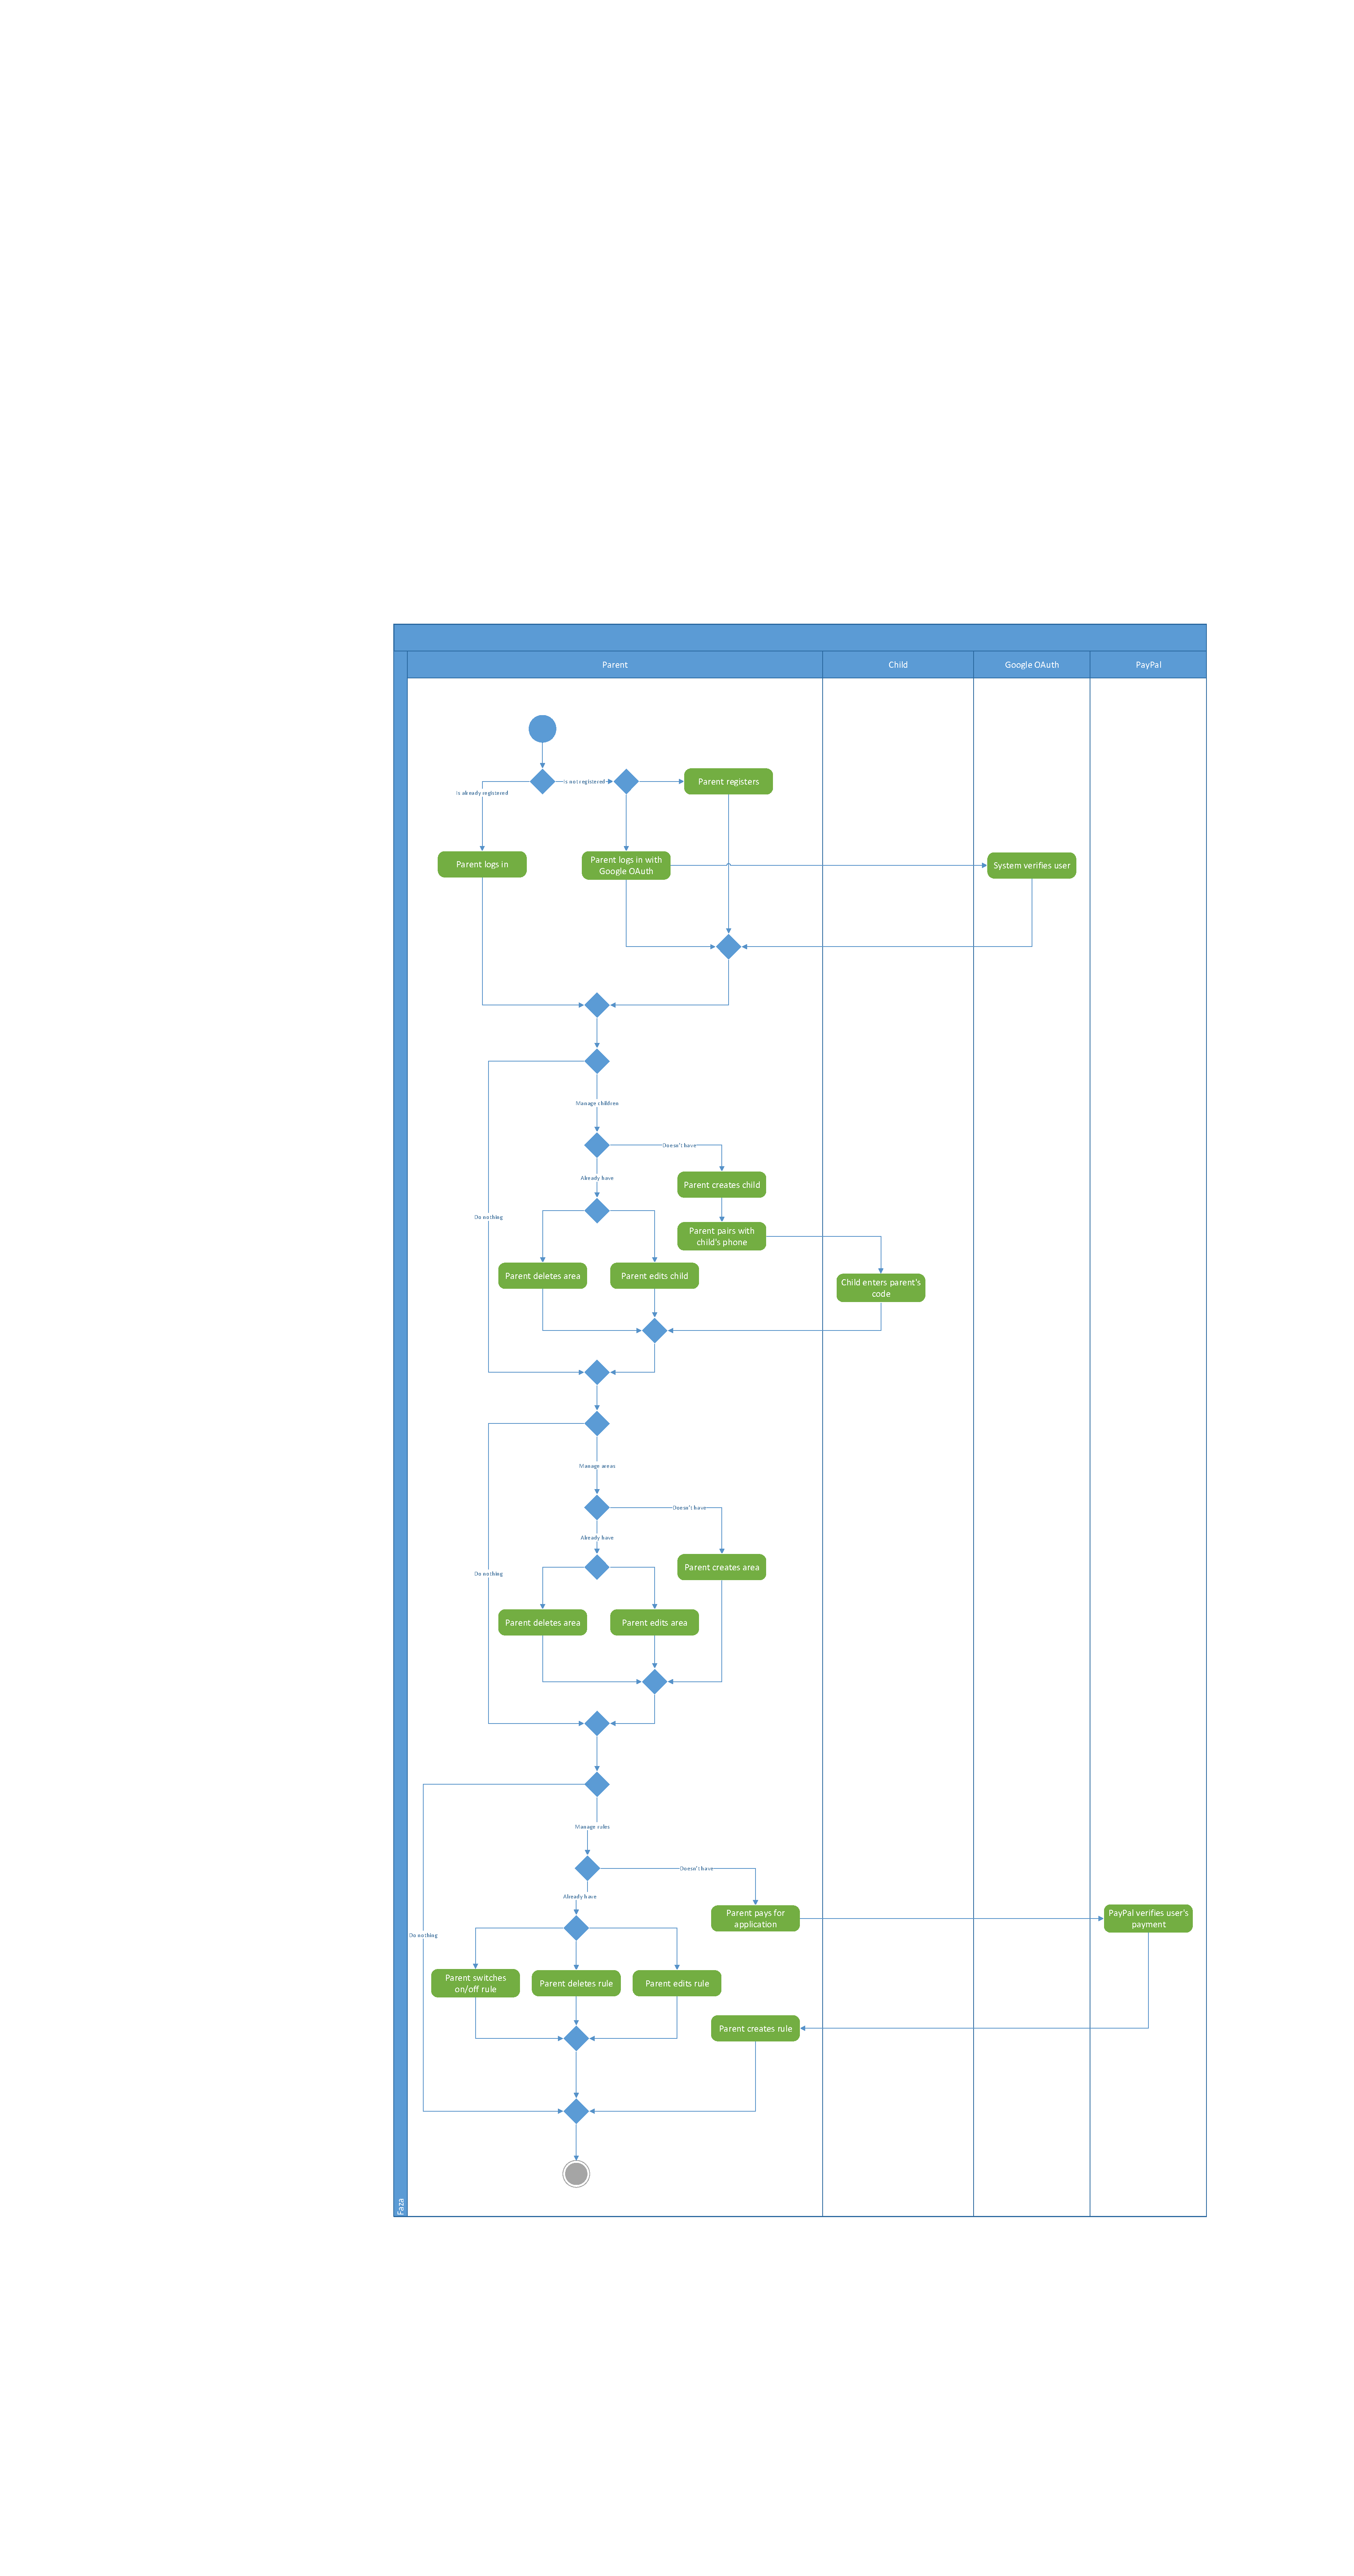
\includegraphics[height=\textheight]{Business_Activity_Diagram} 
				\end{tabular}
				\caption{Business activity diagram}
			\end{figure}

			\begin{figure}[H]
				\centering
				\begin{tabular}{c}
					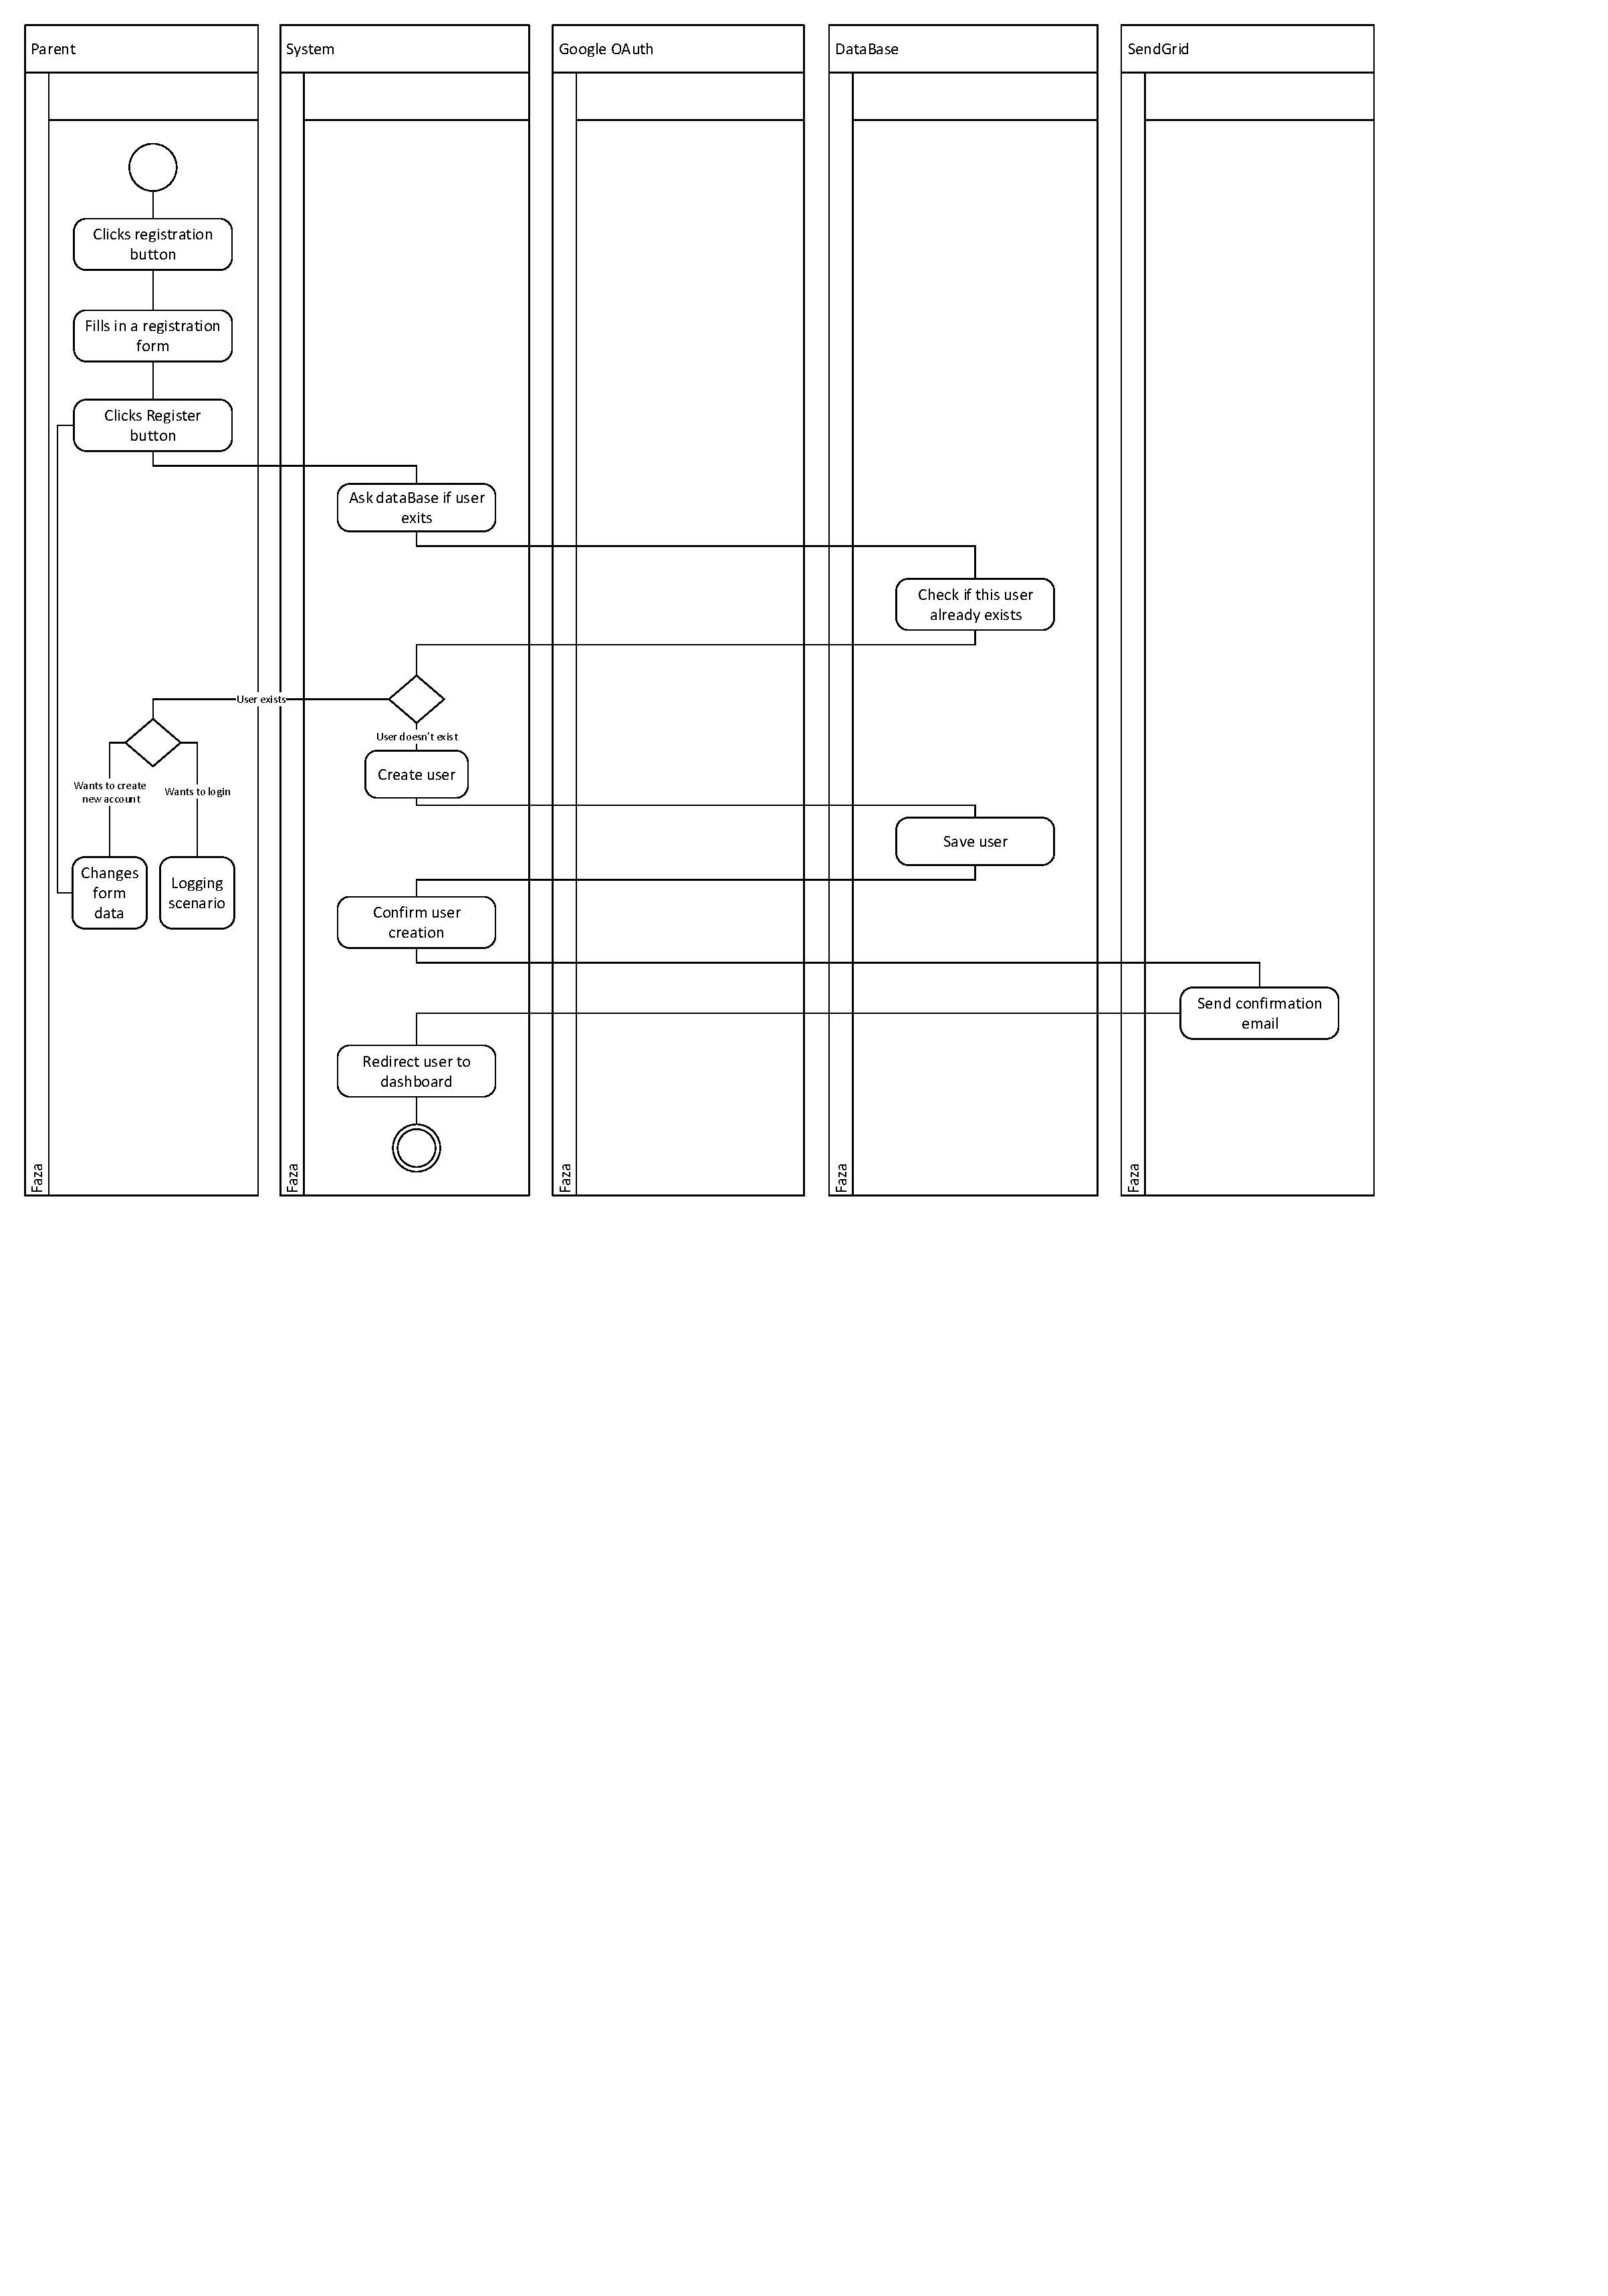
\includegraphics[width=.95\textwidth]{cropped_Registration_Activity_Diagram} 
				\end{tabular}
			\caption{Registration activity diagram}
			\end{figure}

			\begin{figure}[H]
				\centering
				\begin{tabular}{c}
					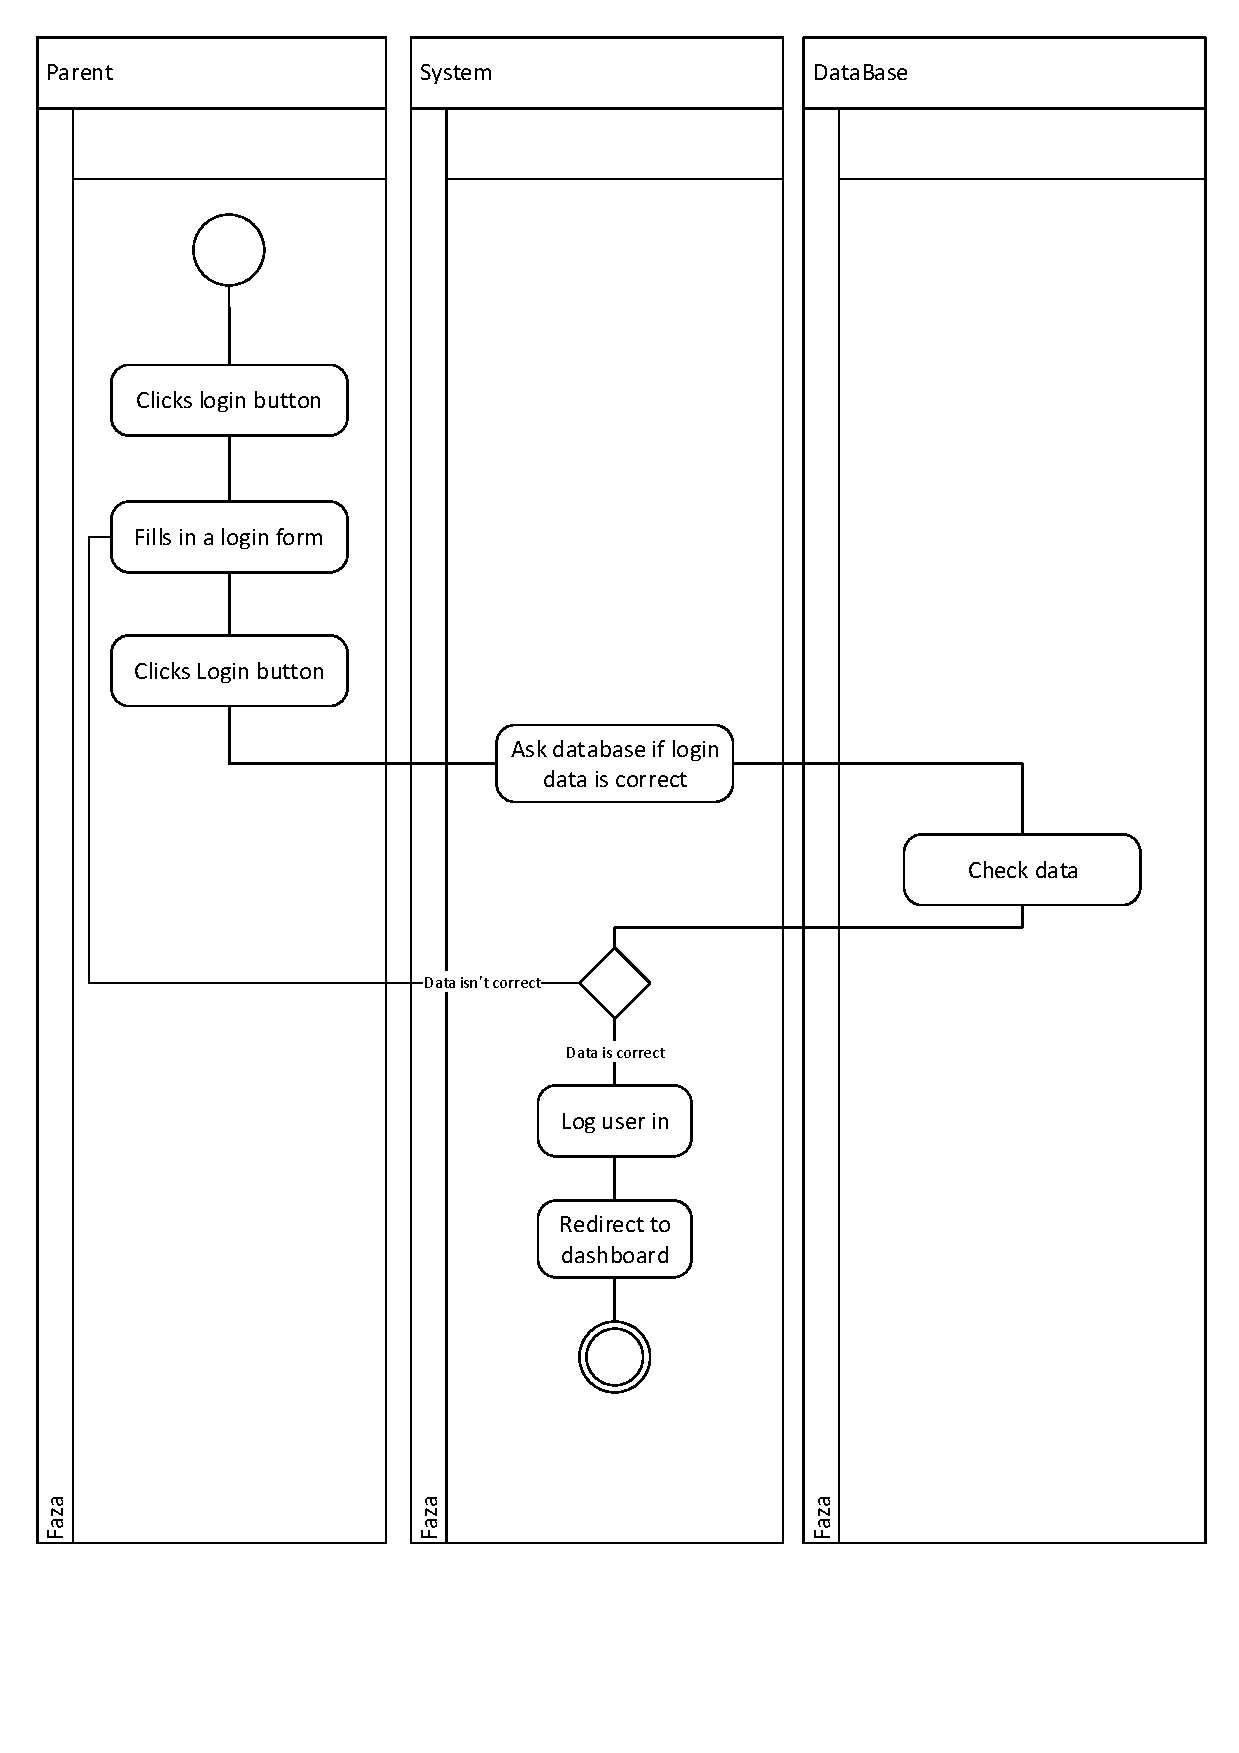
\includegraphics[width=.95\textwidth]{Login_cropped} 
				\end{tabular}
			\caption{Signing in activity diagram}
			\end{figure}

			\begin{figure}[H]
				\centering
				\begin{tabular}{c}
					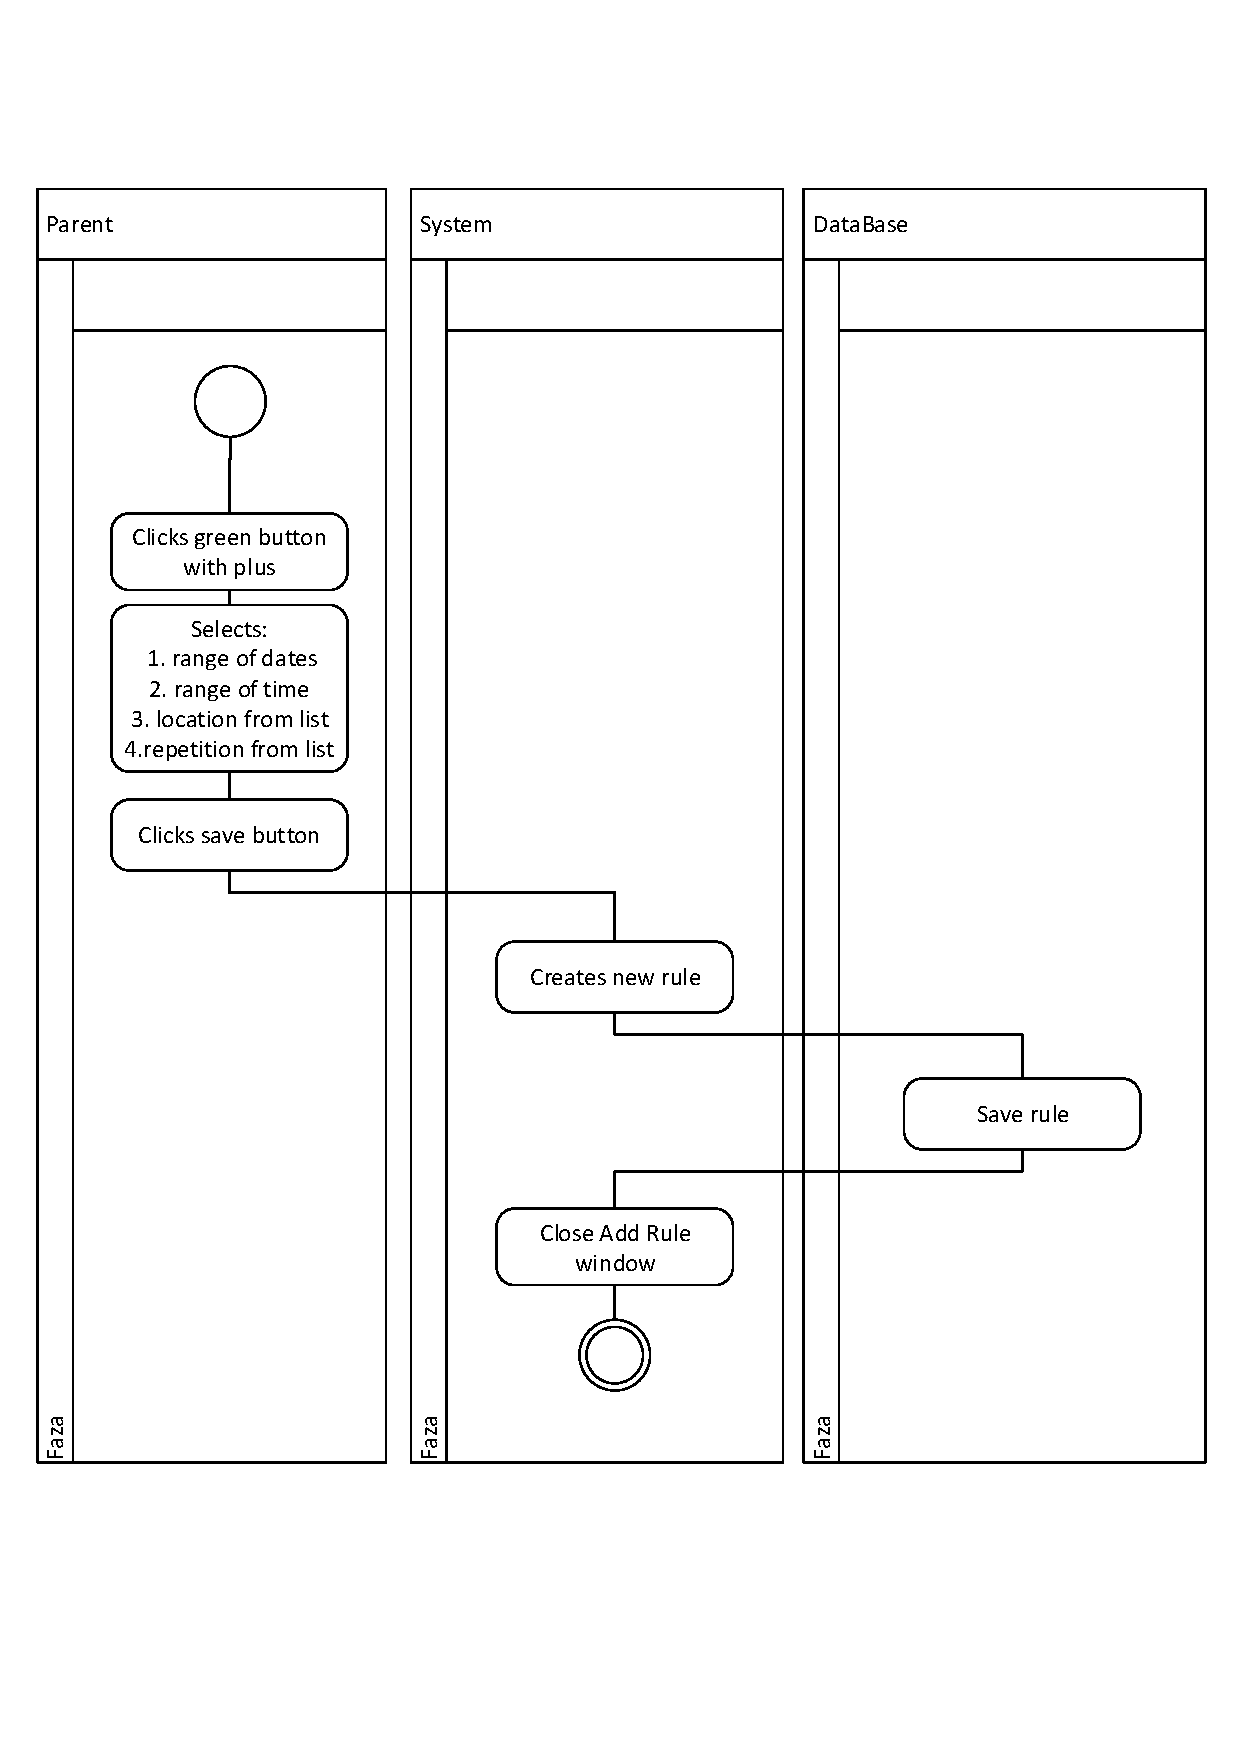
\includegraphics[width=.95\textwidth]{crudCreate_cropped} 
				\end{tabular}
			\caption{Creating new rule activity diagram}
			\end{figure}

			\begin{figure}[H]
				\centering
				\begin{tabular}{c}
					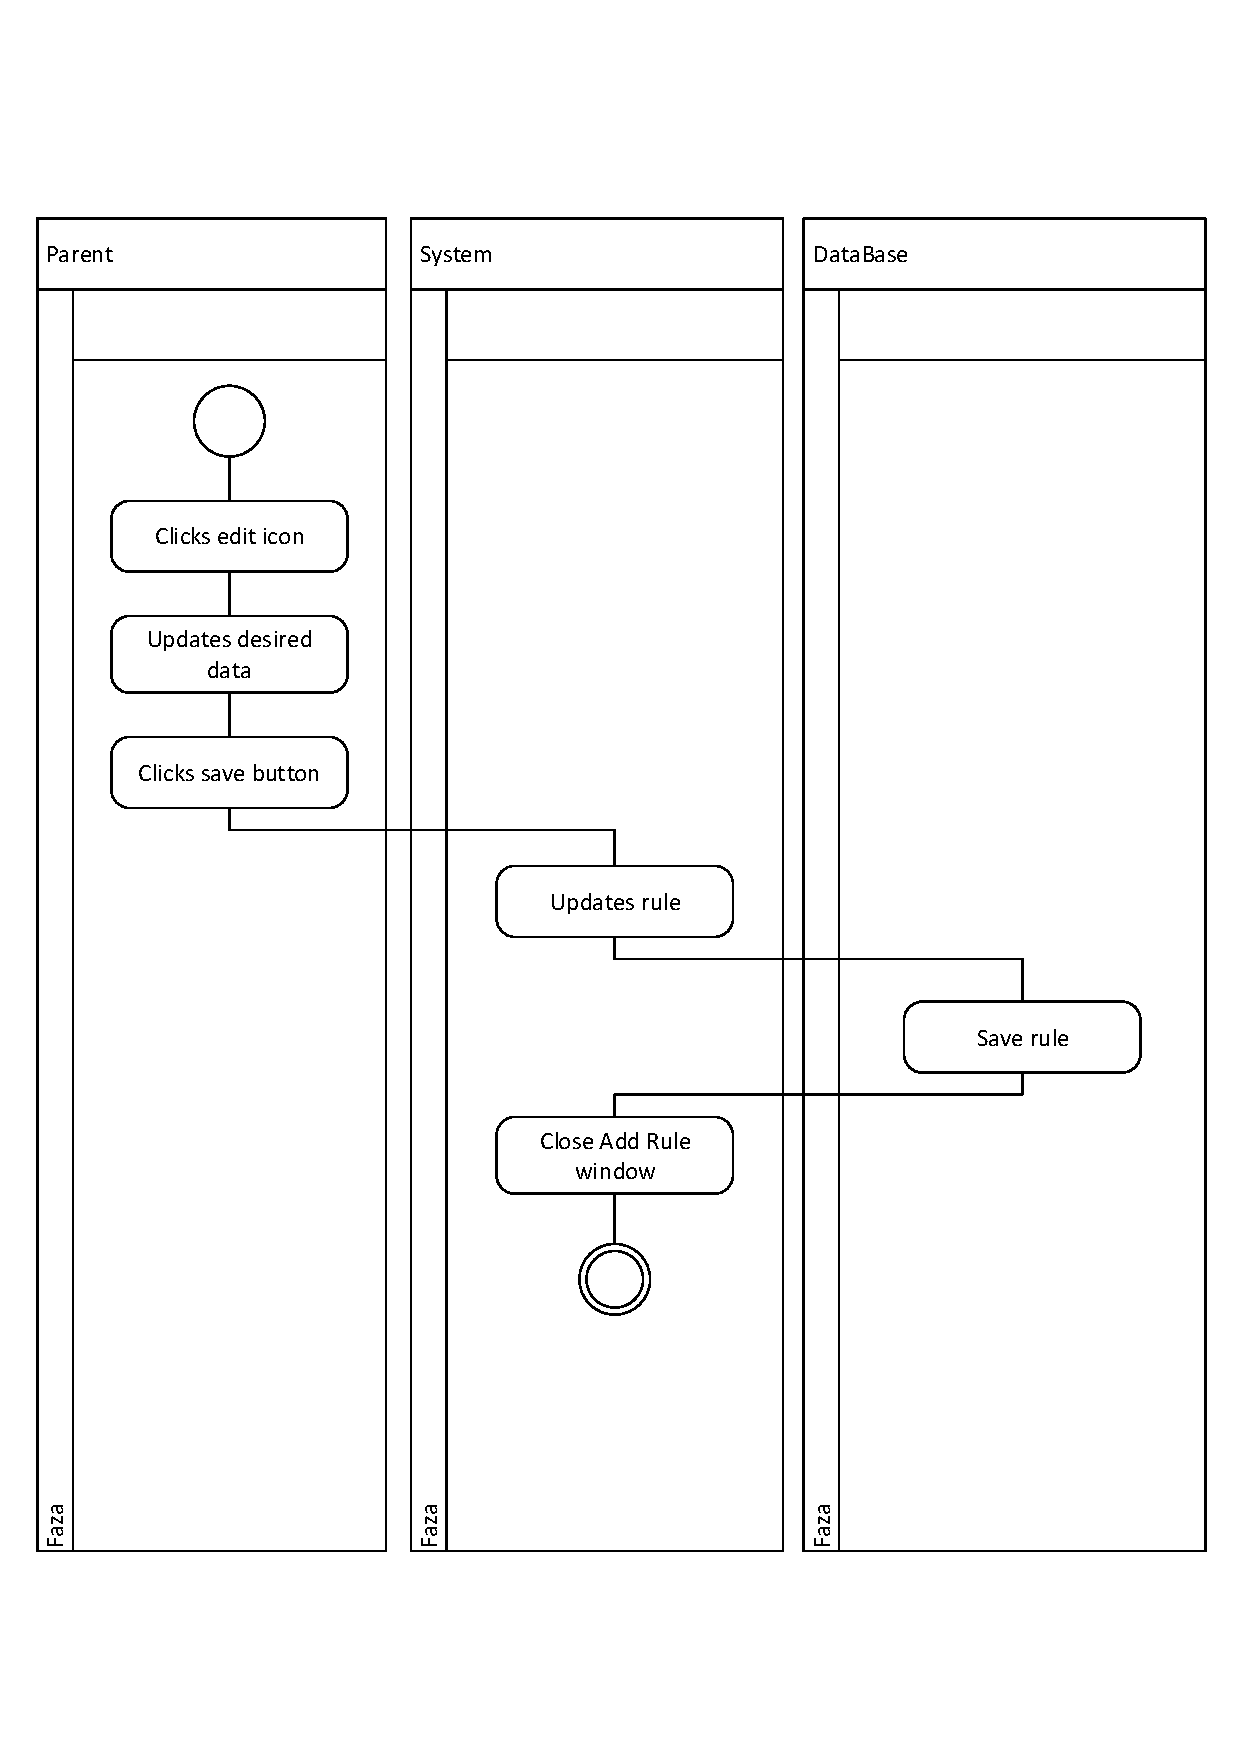
\includegraphics[width=.95\textwidth]{crudUpdate_cropped} 
				\end{tabular}
			\caption{Updating rule activity diagram}
			\end{figure}

			\begin{figure}[H]
				\centering
				\begin{tabular}{c}
					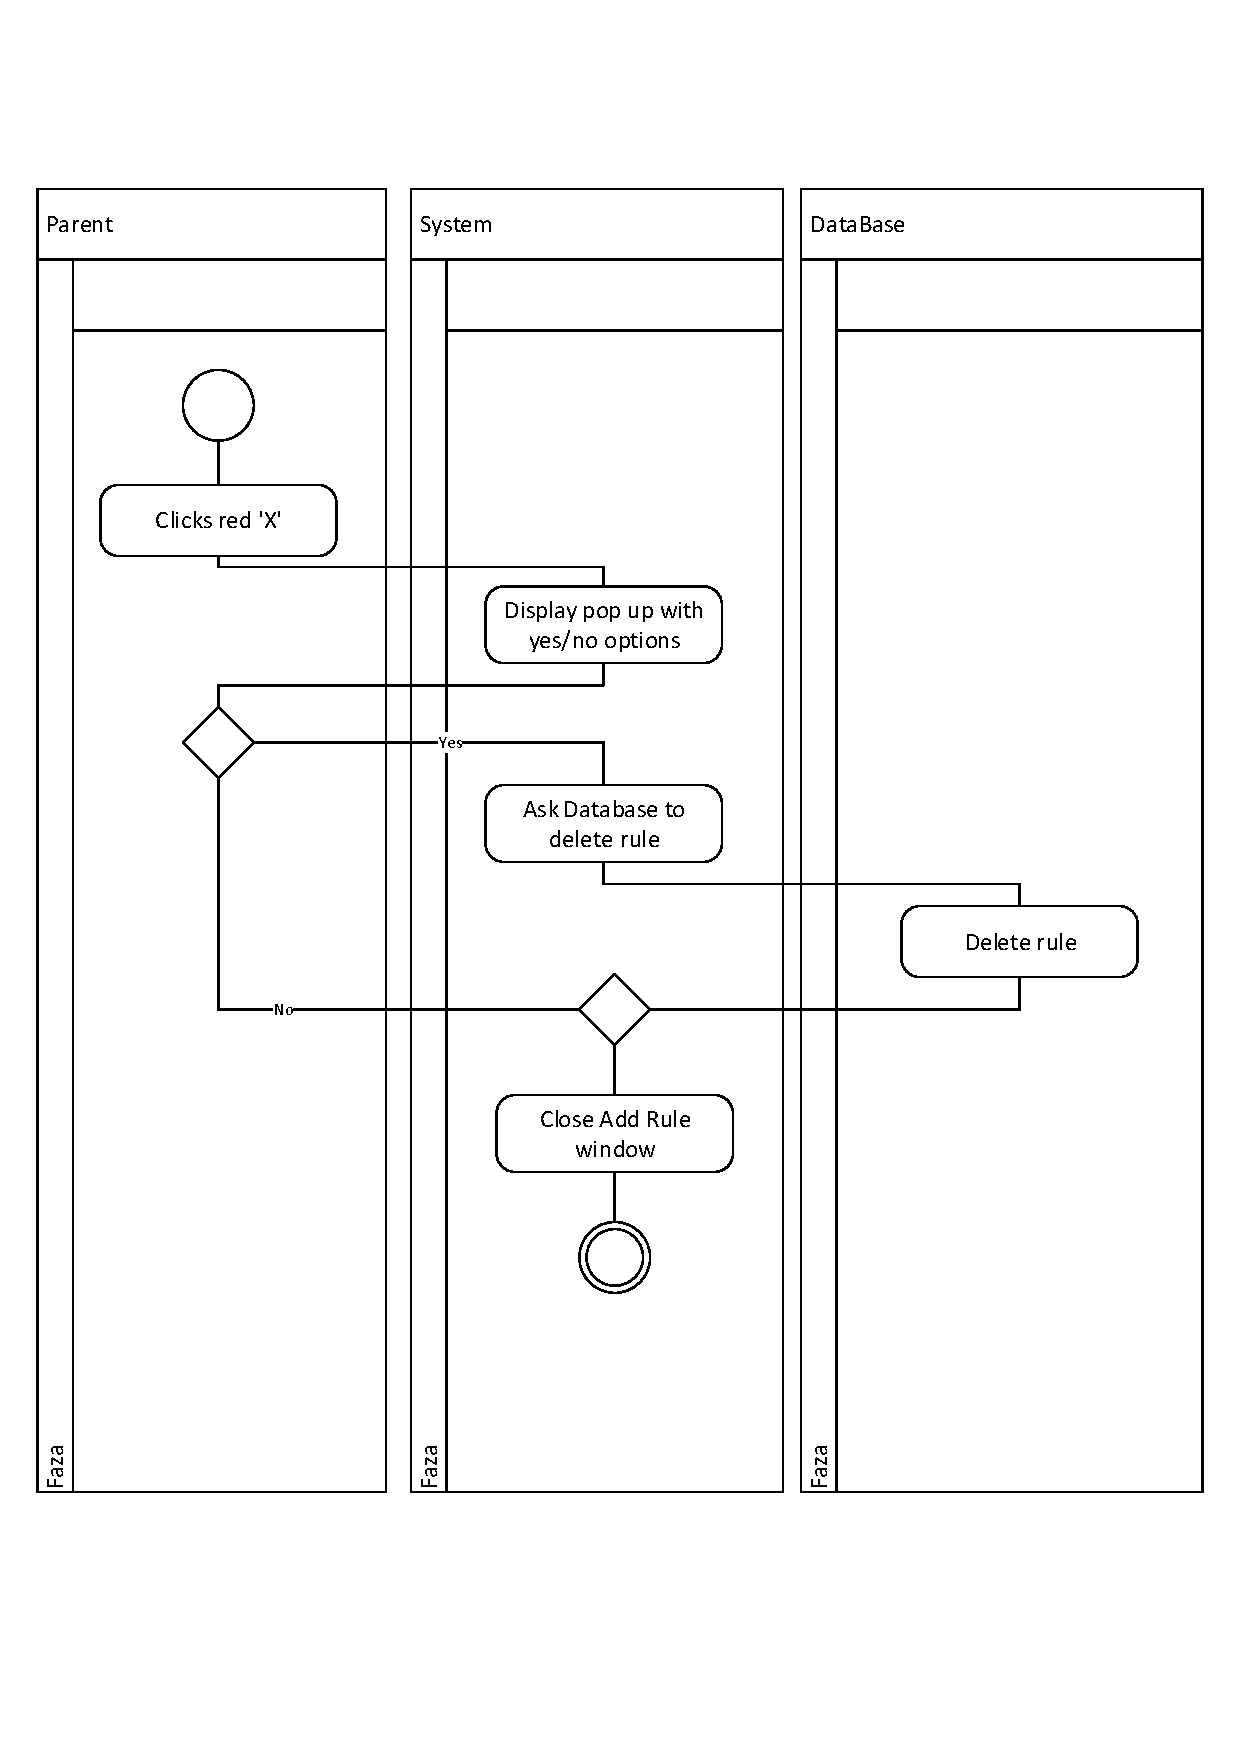
\includegraphics[width=.95\textwidth]{crudDelete_cropped} 
				\end{tabular}
			\caption{Deleting rule activity diagram}
			\end{figure}


			In diagrams we included CRUD operations for rules' management, but didn't include CRUD operations for other components because they are realized in analogous way.

	\section{Domain's analysis}

		Classes identified in domain:
		\begin{itemize}
			\item ParentsAccount - responsible for storing data about parent's account,
			\item ChildsAccount - responsible for storing data about child's account,
			\item Rule - responsible for storing data about rules concerning children, area, and time in which rule is active, 
			\item Location - class directly connected with child's account, storing data about current location of child,
			\item Area Interface - interface for Area's classes,
			\item CircularArea - class responsible for storing data about center and radius of area.
		\end{itemize}

		\begin{figure}[H]
			\centering
			\begin{tabular}{c}
				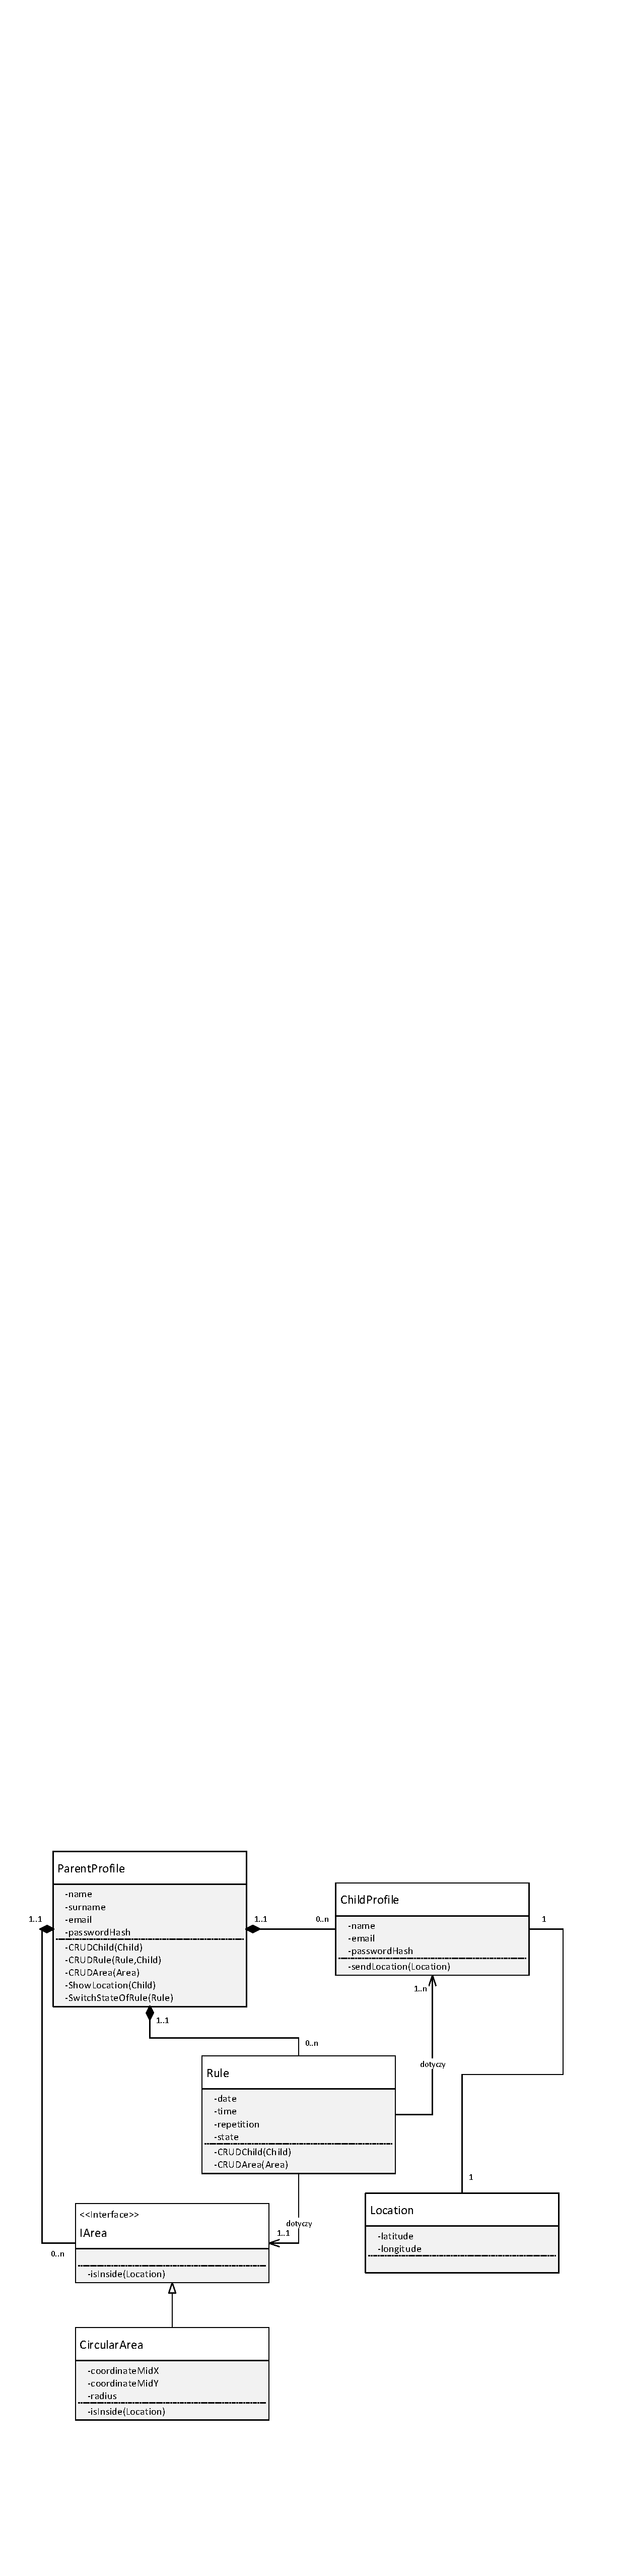
\includegraphics[width=.95\textwidth]{classes} 
			\end{tabular}
		\caption{Classes diagram}
		\end{figure}
	
		\subsection{State diagrams}
		
		\begin{figure}[H]
			\centering
			\begin{tabular}{c}
				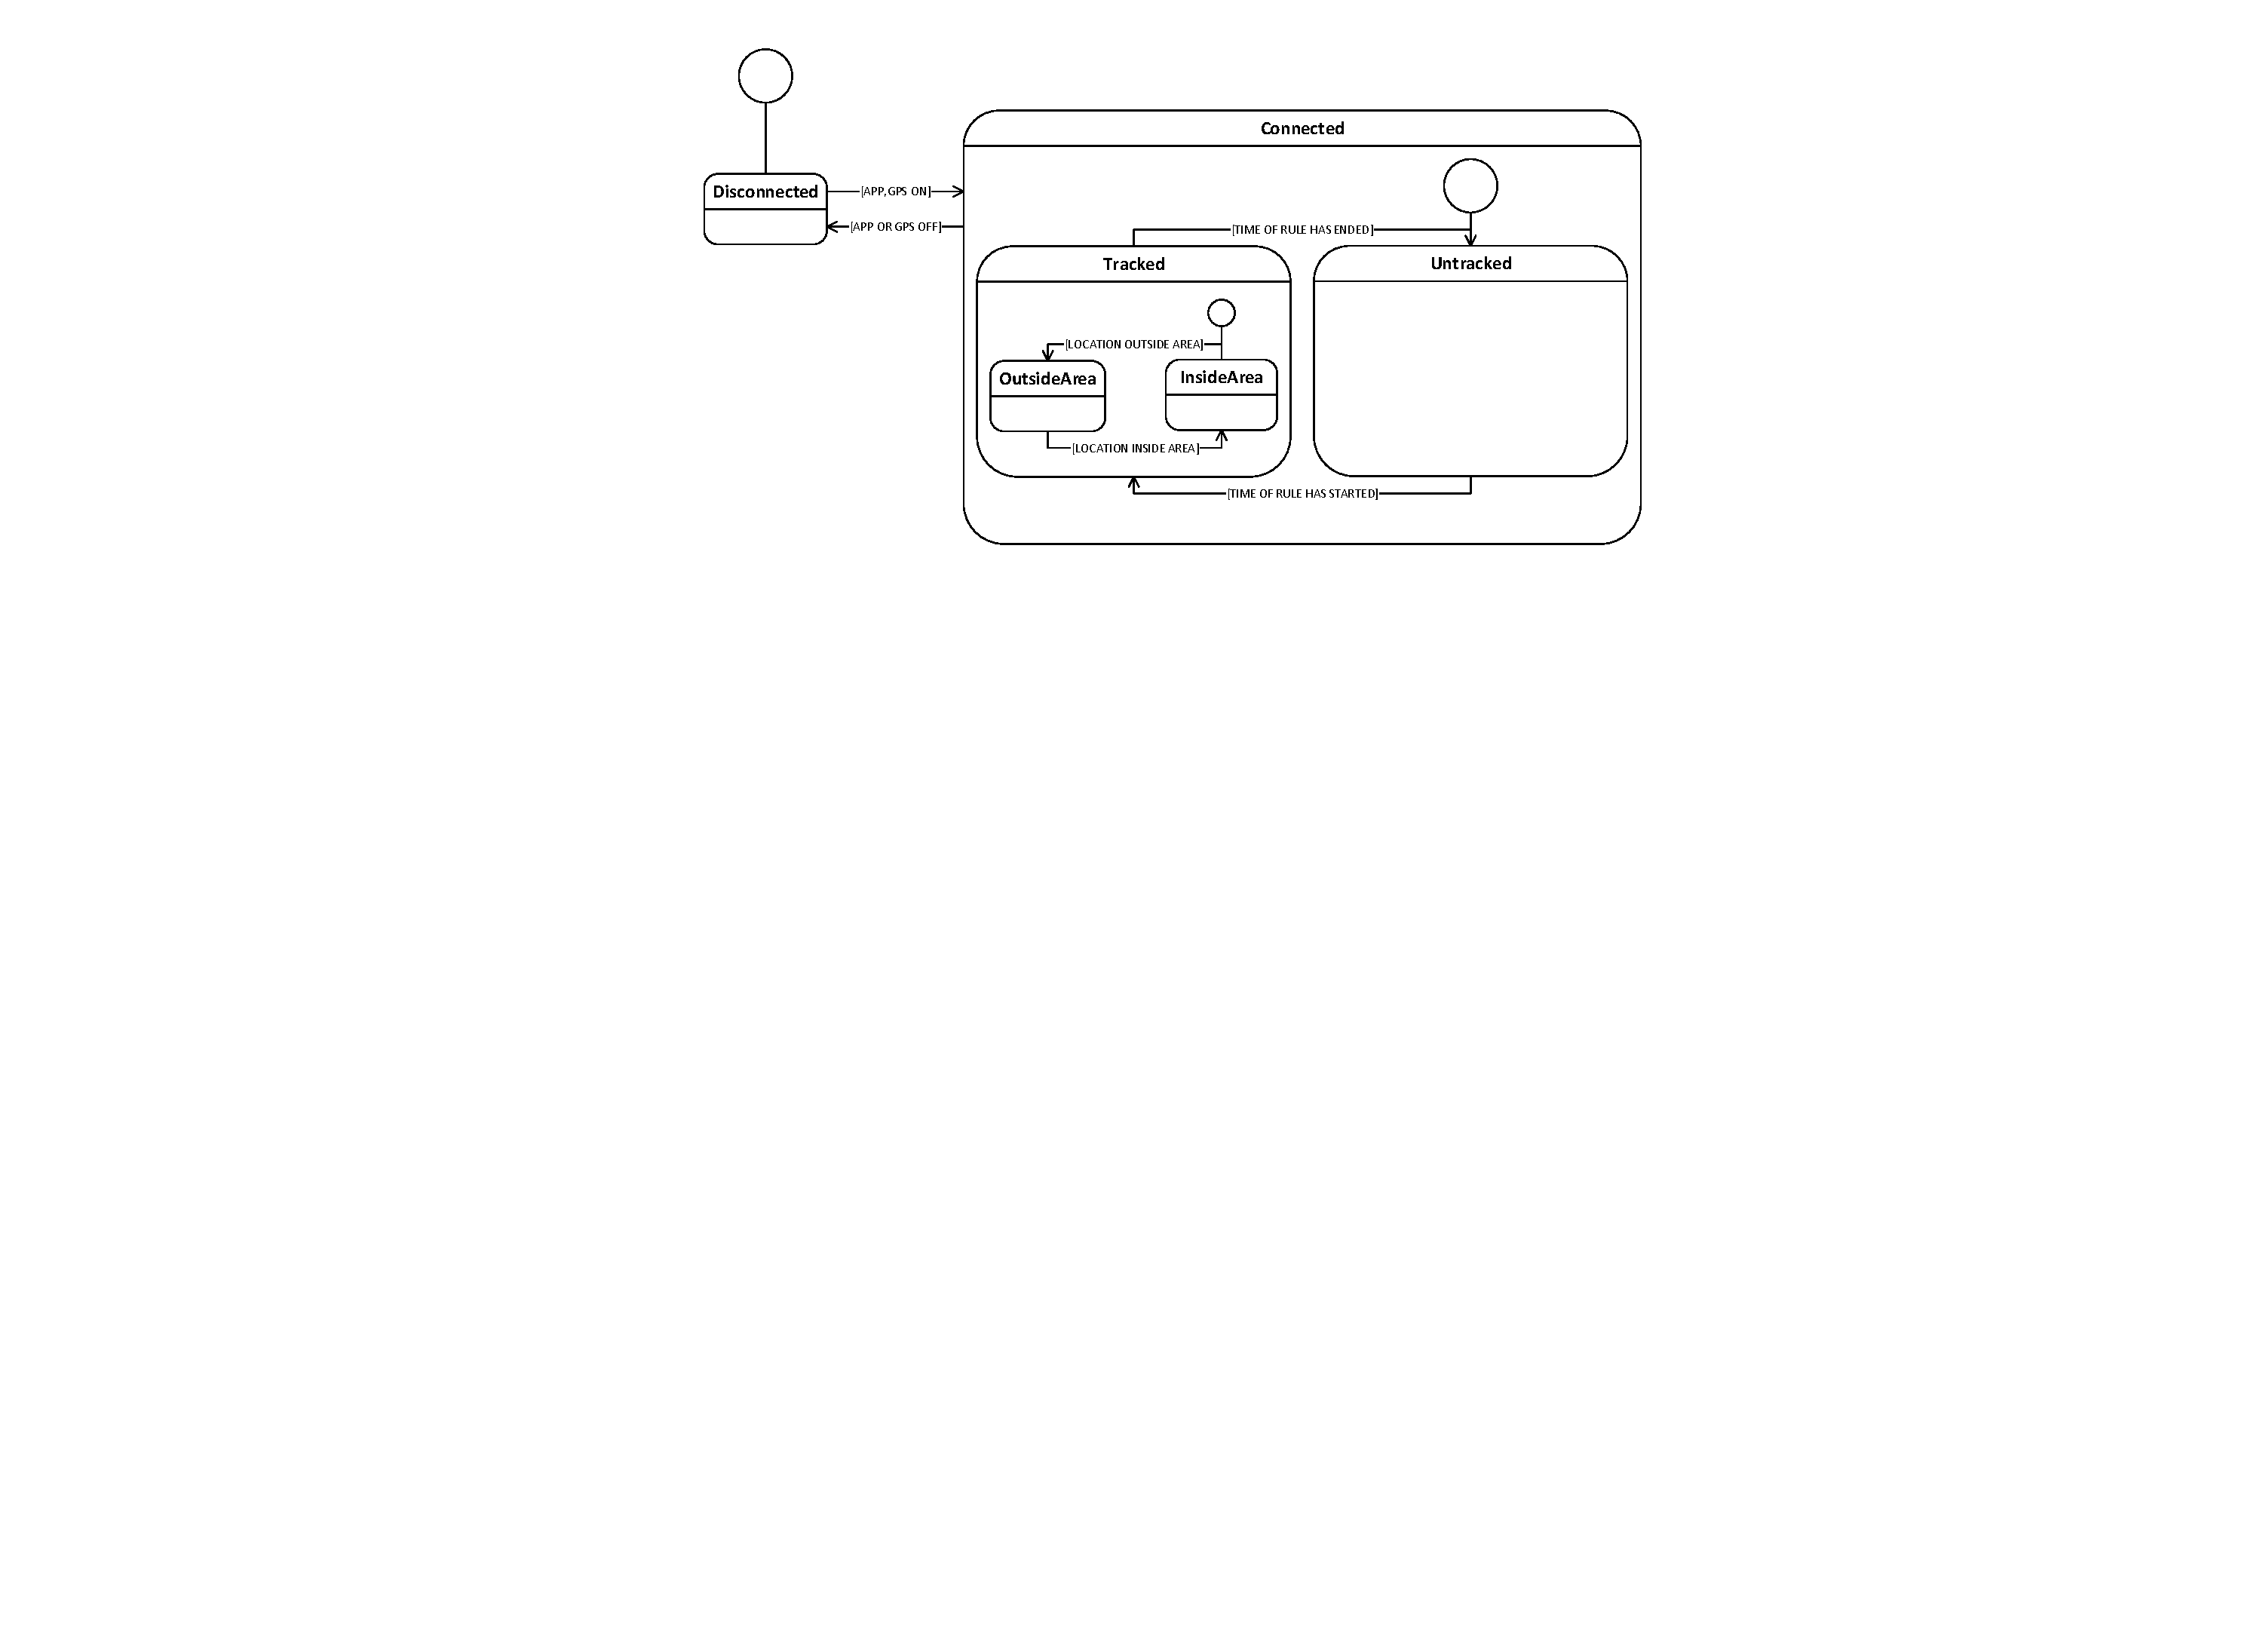
\includegraphics[width=.95\textwidth]{Stanu_cropped} 
			\end{tabular}
			\caption{State diagram for child's application}
		\end{figure}
 
		\begin{figure}[H]
			\centering 
			\begin{tabular}{c}
				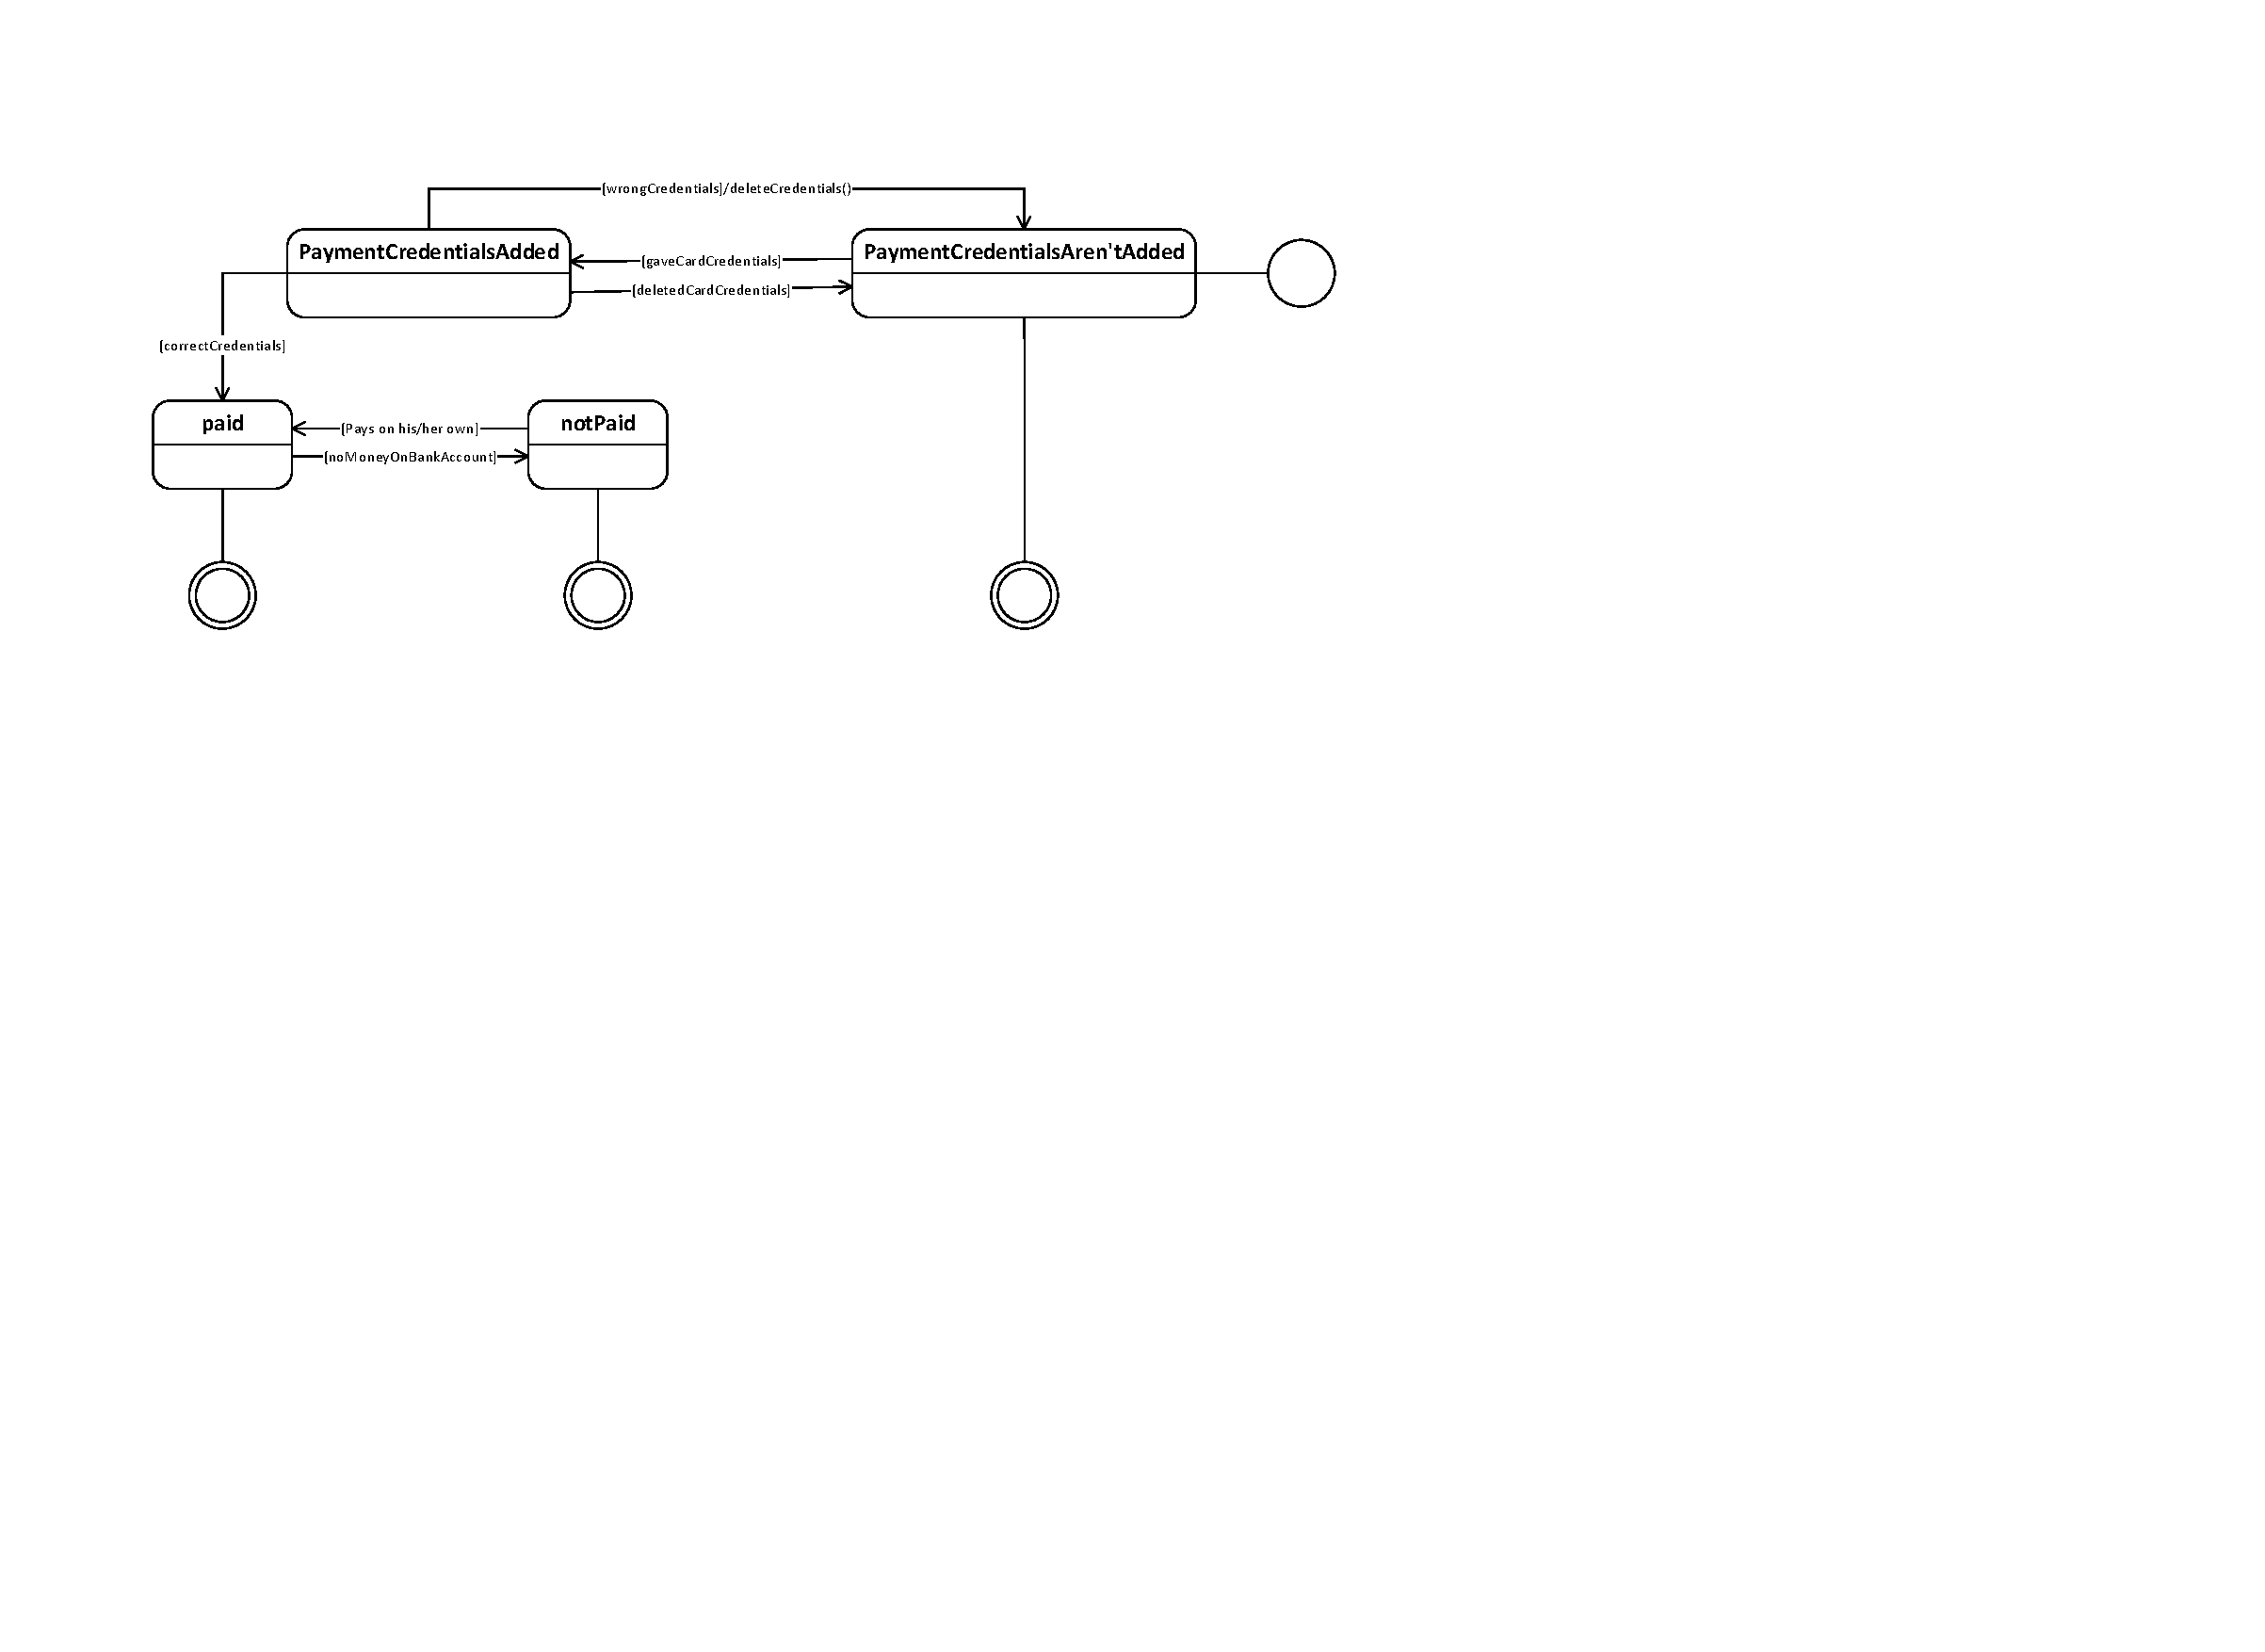
\includegraphics[width=.95\textwidth]{paymentStateDiagram} 
			\end{tabular}
			\caption{State diagram for payment}
		\end{figure}
 
	\section{Requirements' specification}
		
		Requirements was shown in form of use cases with scenarios. We aren't showing scenarios for mobile application's use cases because they are too trivial.

		\begin{figure}[H] 
			\centering
			\begin{tabular}{c}
				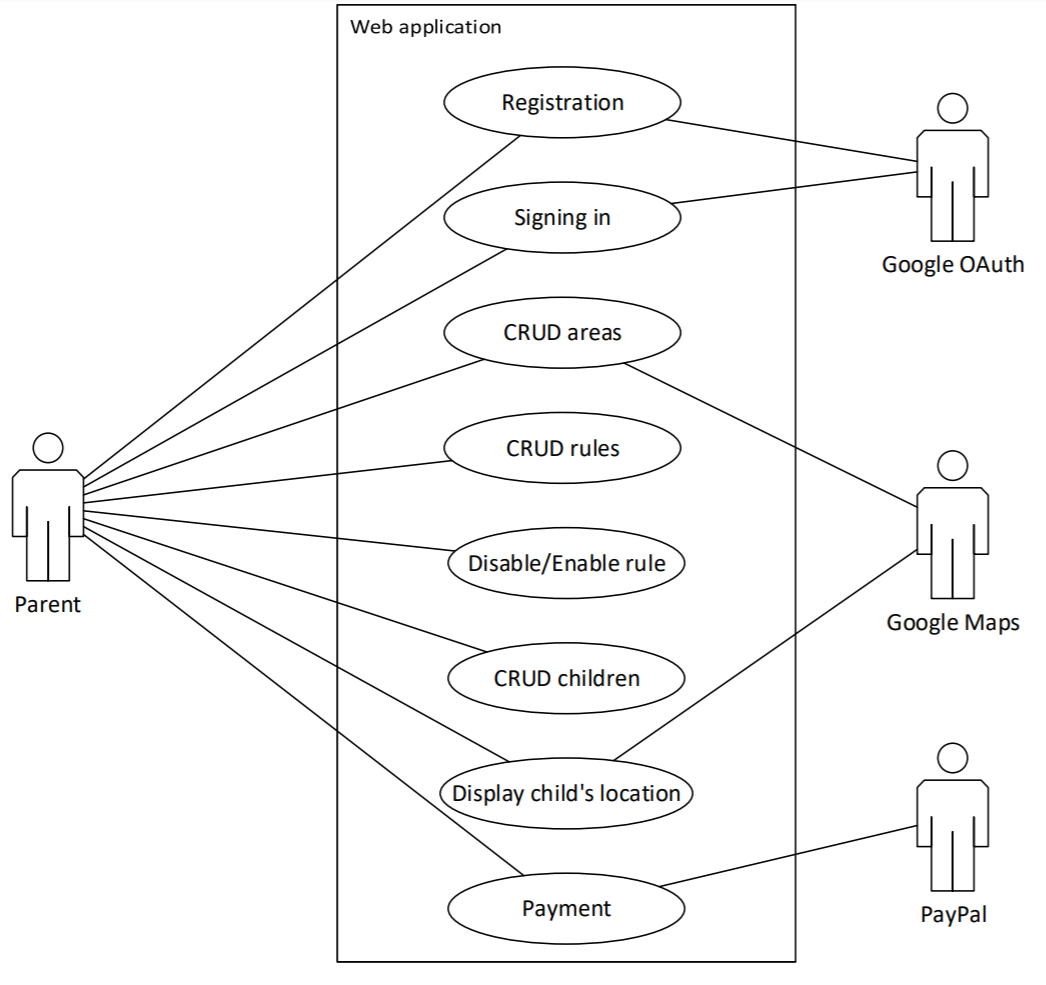
\includegraphics[width=.80\textwidth]{webUseCase} 
			\end{tabular} 
		\caption{Use cases for web application}
		\end{figure}

		\begin{figure}[H]
			\centering
			\begin{tabular}{c}
				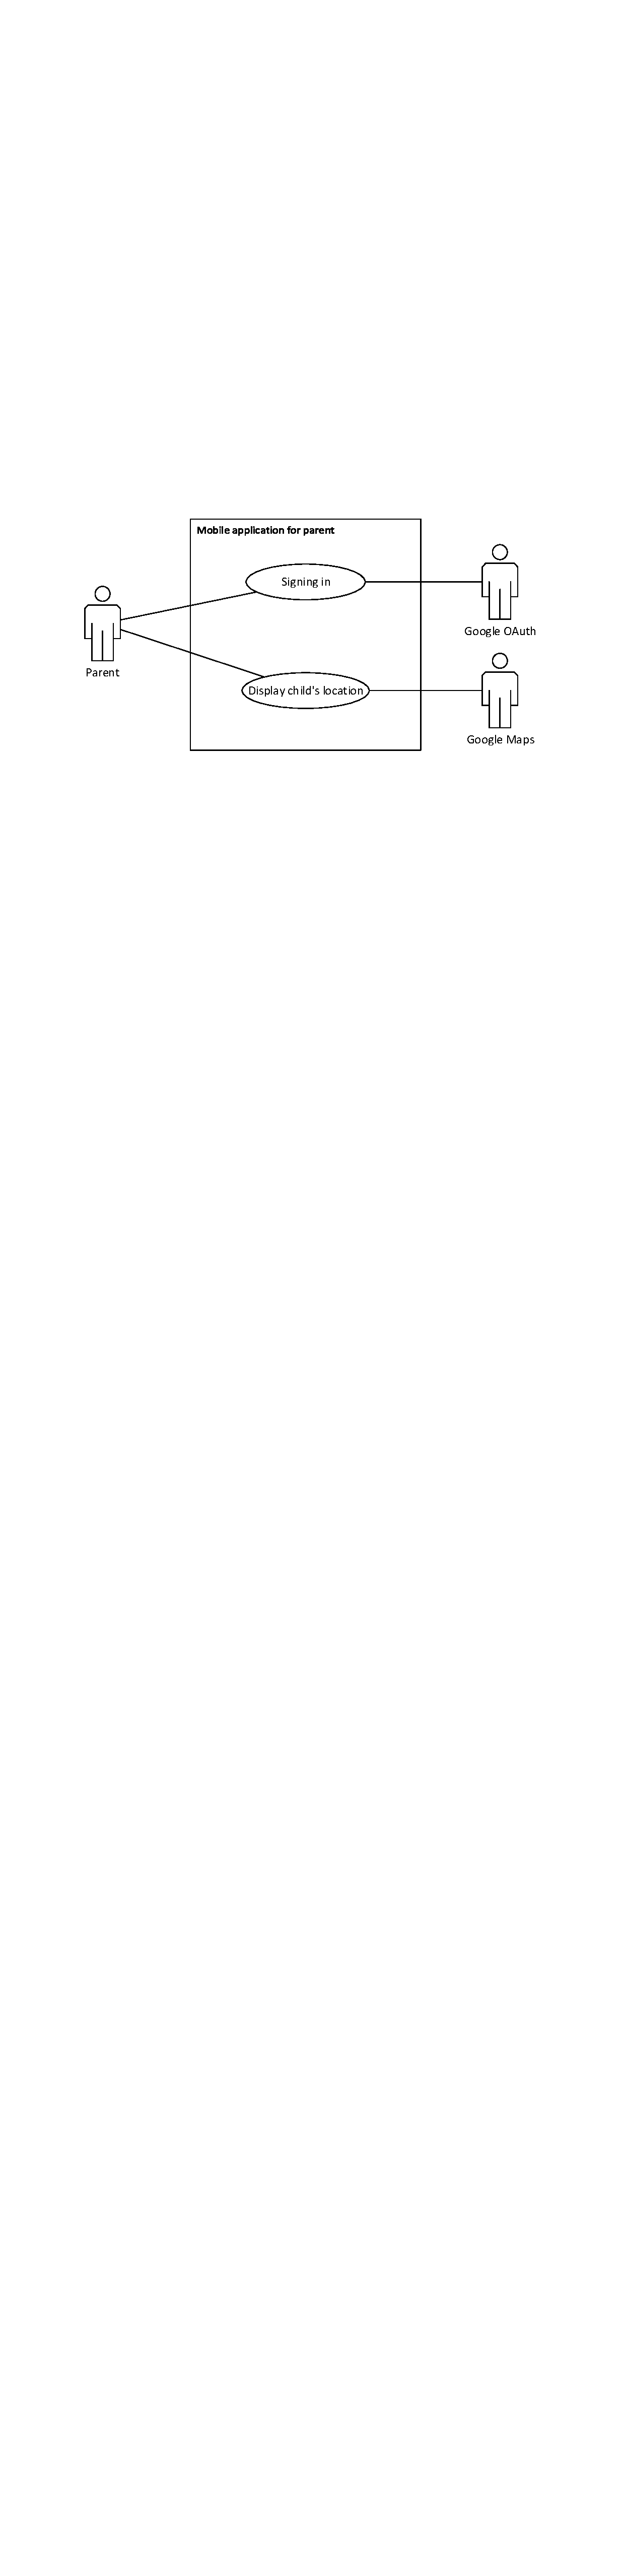
\includegraphics[width=.80\textwidth]{parentUseCase} 
			\end{tabular} 
		\caption{Use cases for parent's mobile application}
		\end{figure} 

		\begin{figure}[H] 
			\centering
			\begin{tabular}{c}
				
\includegraphics[width=.80\textwidth]{childUseCase} 
			\end{tabular} 
		\caption{Use cases for child's mobile application}
		\end{figure}

		\begin{figure}[H] 
			\centering
			\begin{tabular}{c}
				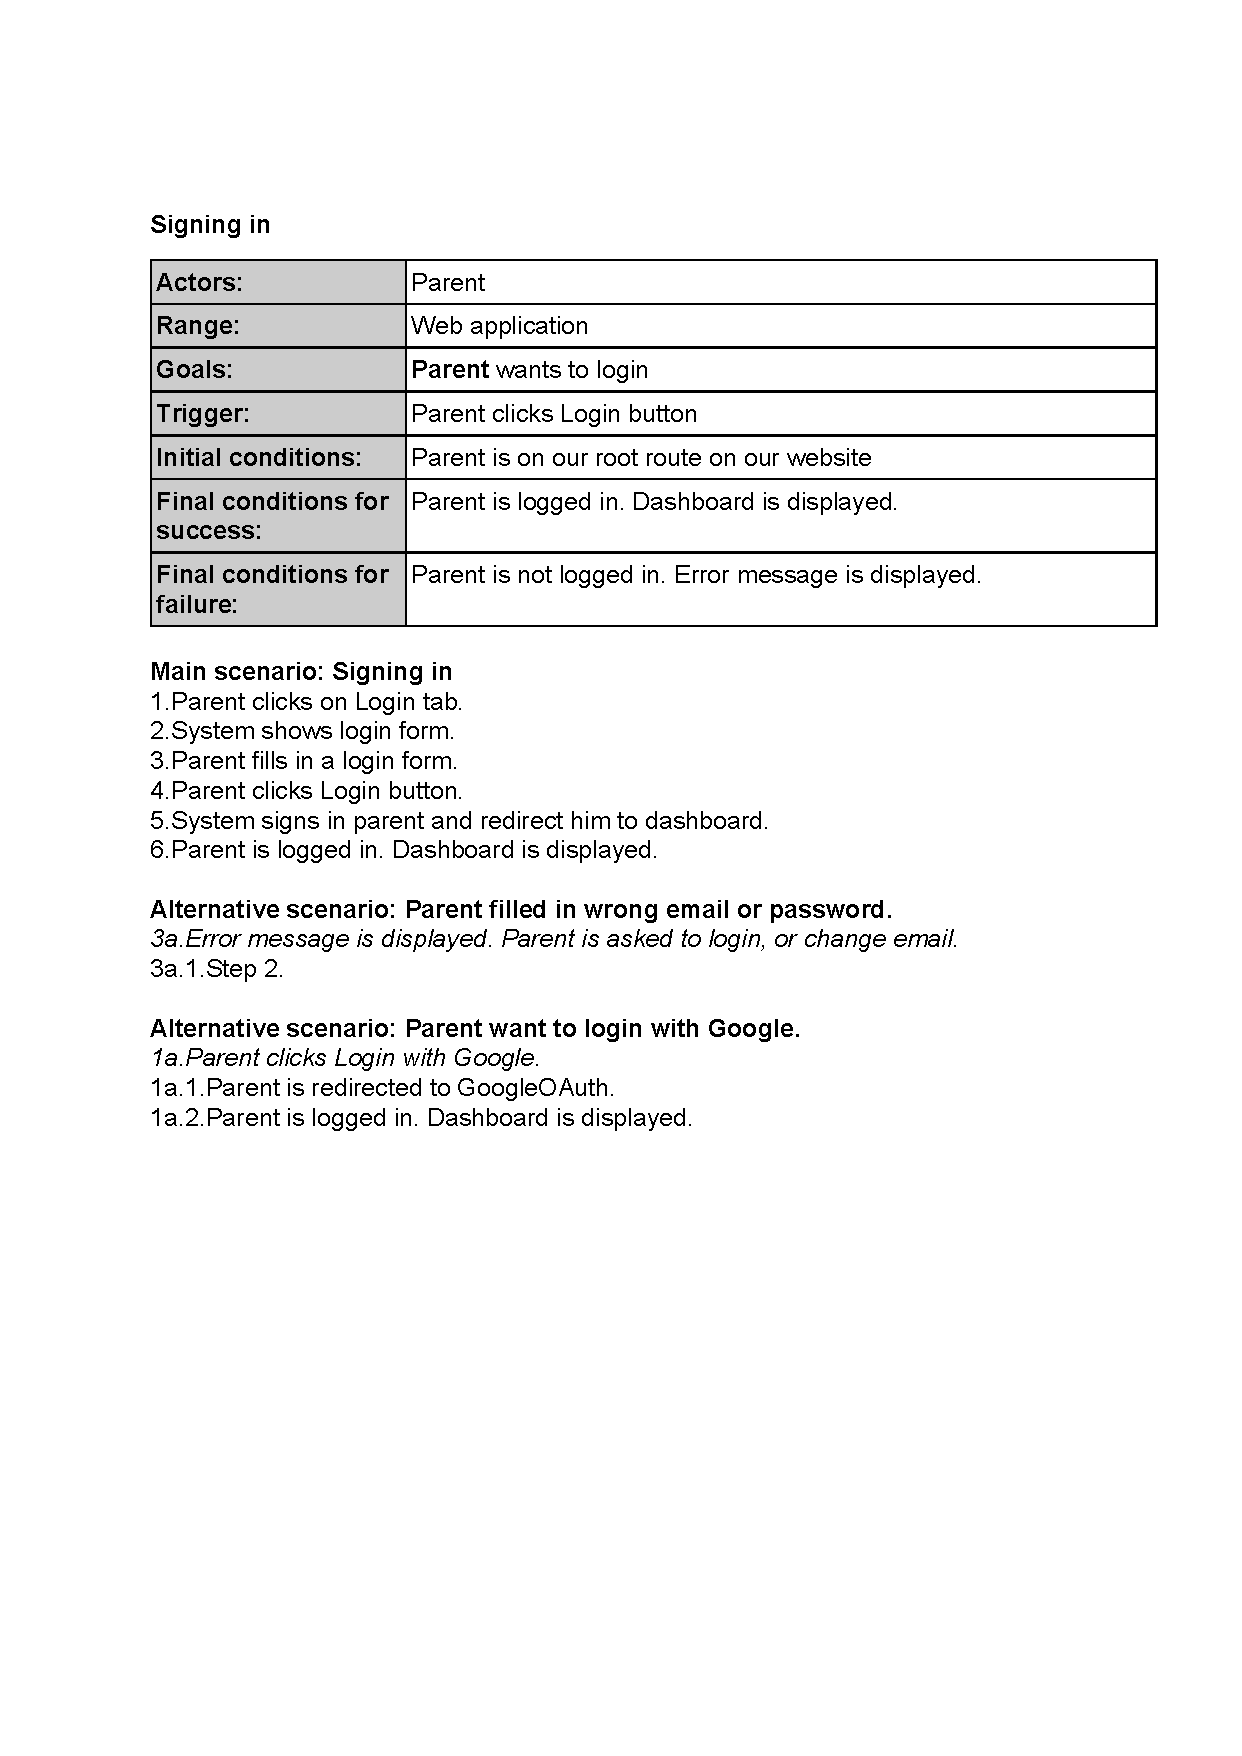
\includegraphics[width=.80\textwidth]{log_cropped} 
			\end{tabular} 
		\caption{Signing in scenario}
		\end{figure}

		\begin{figure}[H]
			\centering
			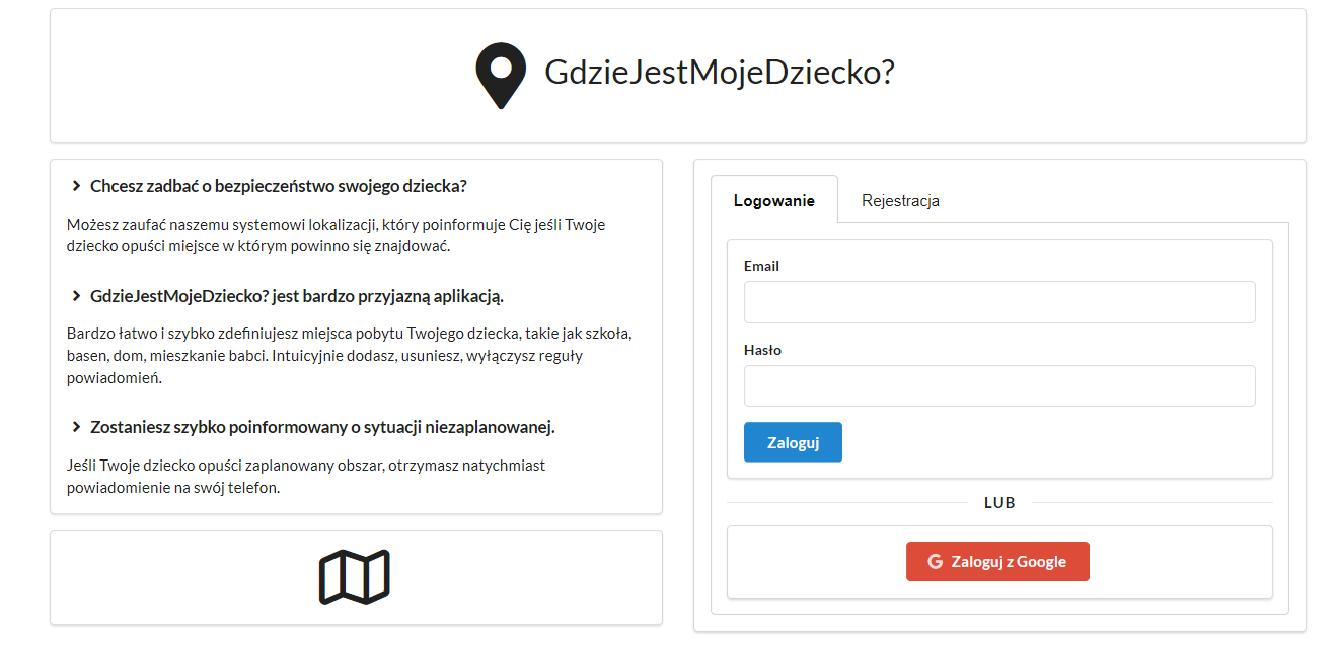
\includegraphics[width=.80\textwidth]{signinIn}
			\caption{Signing in}
		\end{figure}

		\begin{figure}[H] 
			\centering
			\begin{tabular}{c}
				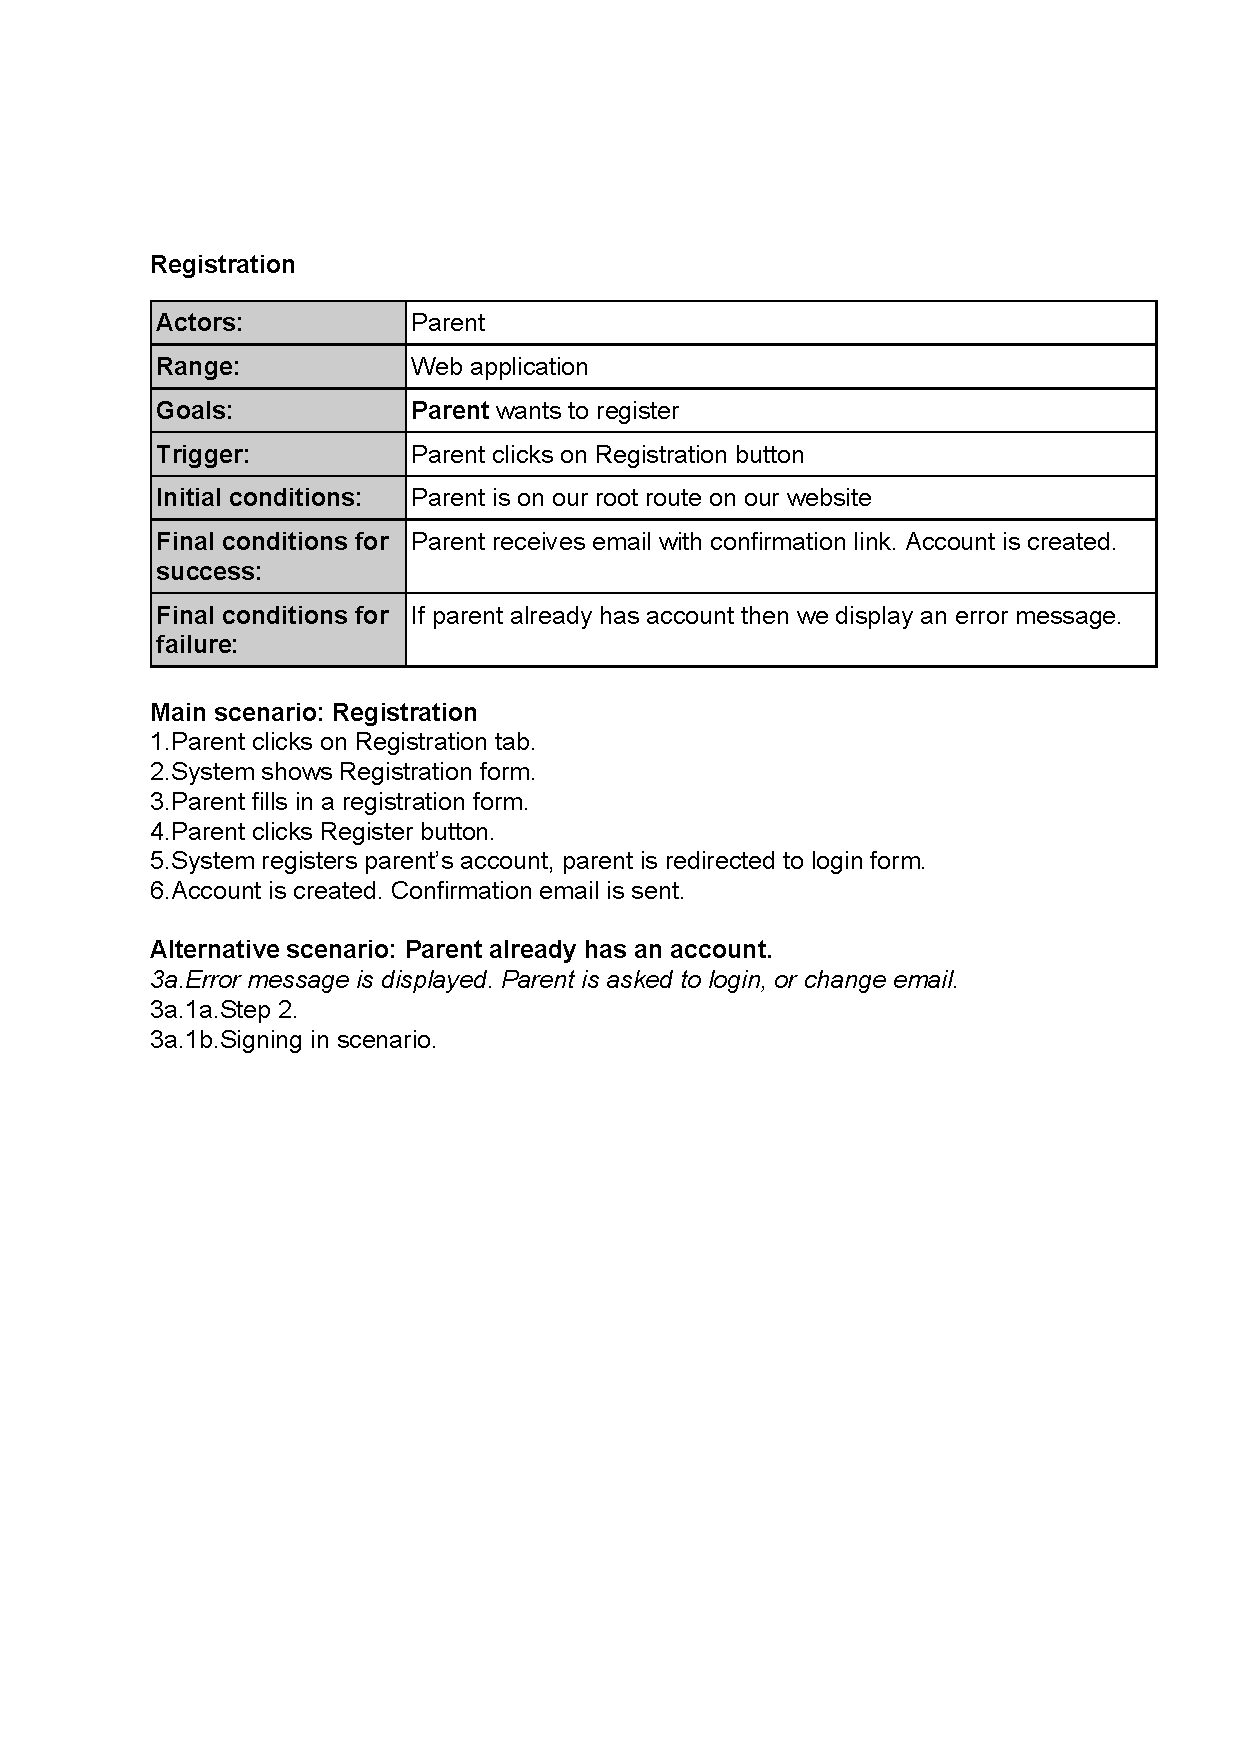
\includegraphics[width=.80\textwidth]{reg_cropped} 
			\end{tabular} 
		\caption{Registration scenario}
		\end{figure}

		\begin{figure}[H]
			\centering
			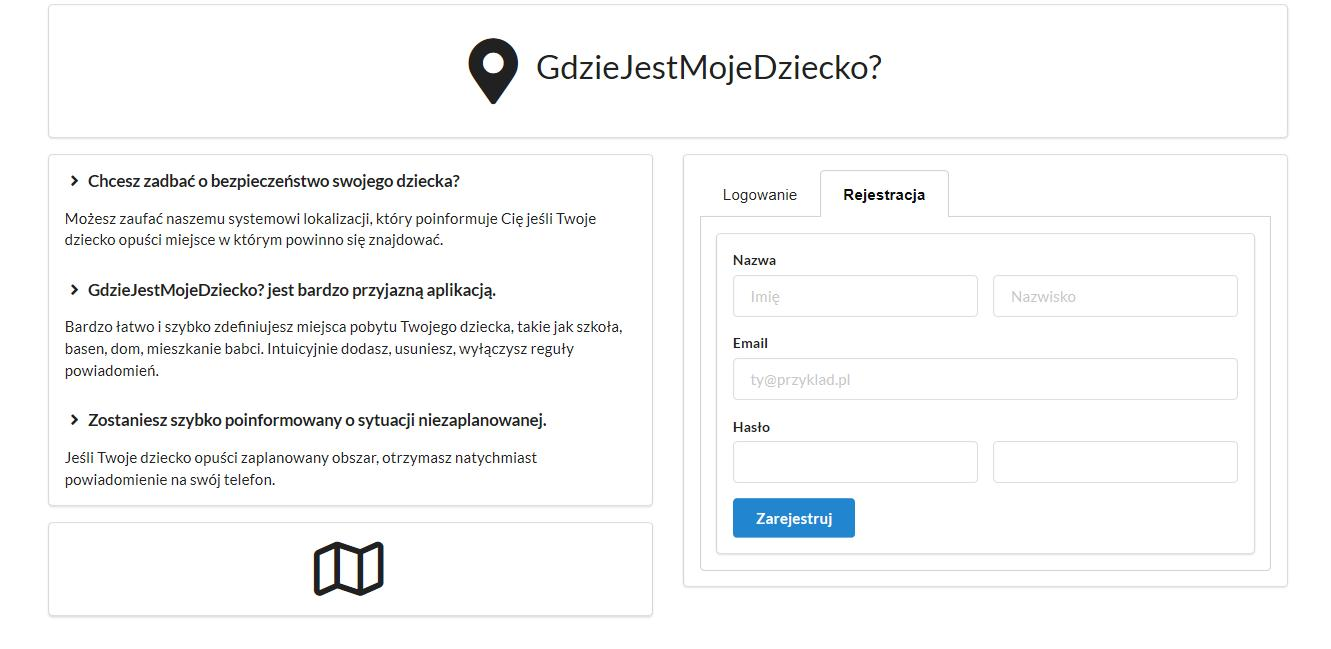
\includegraphics[width=.80\textwidth]{register}
			\caption{Registering}
		\end{figure}

		\begin{figure}[H]
			\centering
			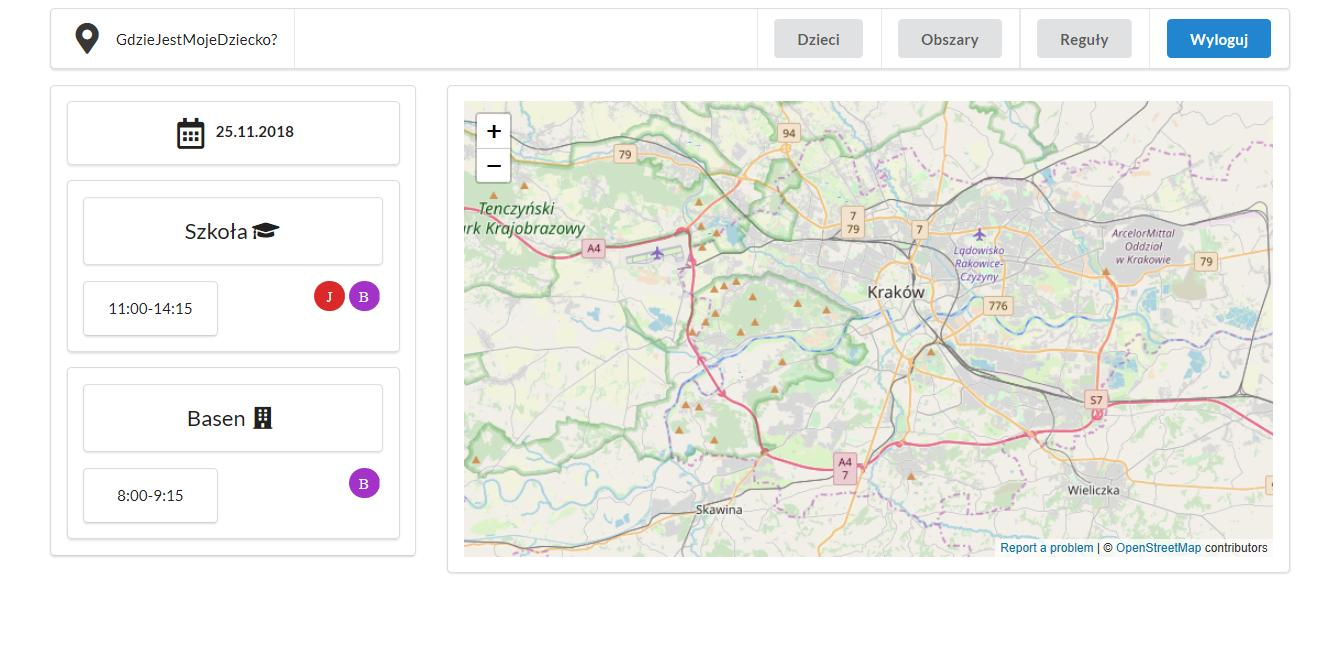
\includegraphics[width=.80\textwidth]{dashboard}
			\caption{Dashboard}
		\end{figure}

		\begin{figure}[H]
			\centering
			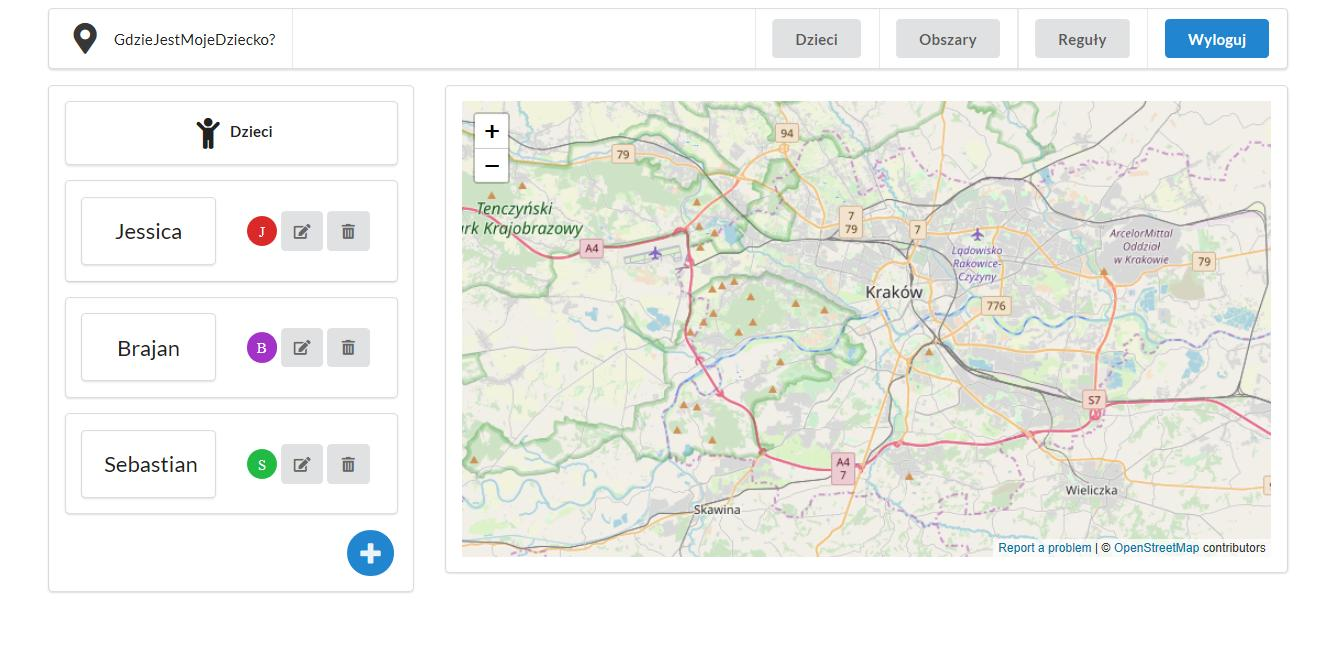
\includegraphics[width=.80\textwidth]{children}
			\caption{Children}
		\end{figure}

		\begin{figure}[H] 
			\centering
			\begin{tabular}{c}
				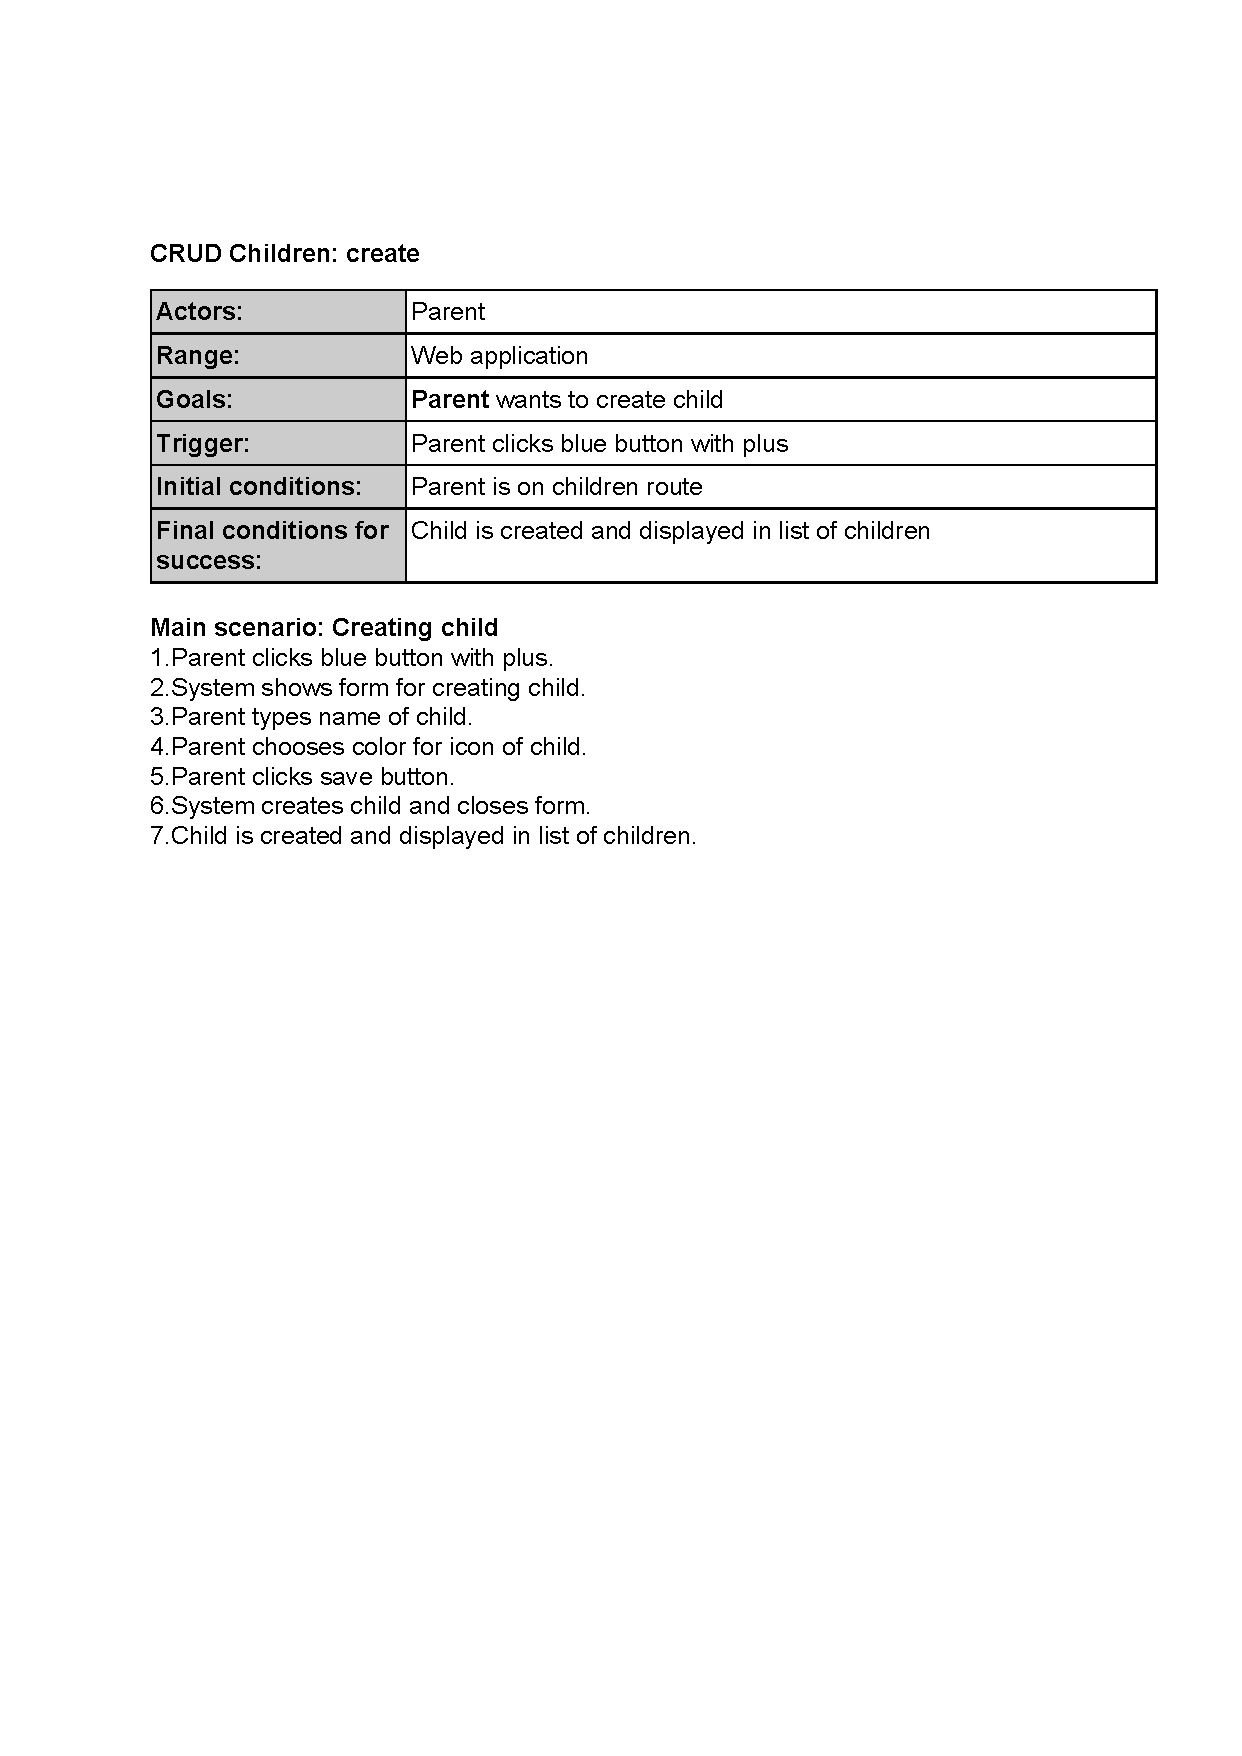
\includegraphics[width=.80\textwidth]{crC_cropped} 
			\end{tabular} 
		\caption{Creating child scenario}
		\end{figure}

		\begin{figure}[H]
			\centering
			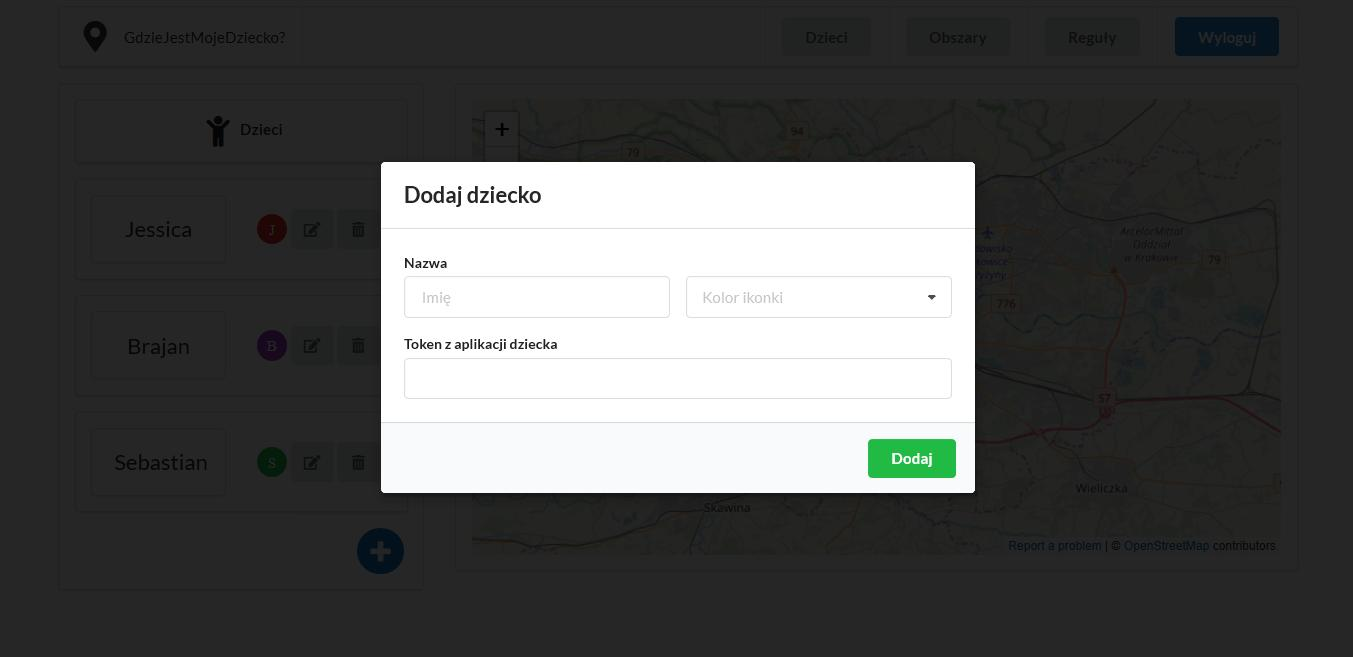
\includegraphics[width=.80\textwidth]{addChild}
			\caption{Creating child}
		\end{figure}

		\begin{figure}[H] 
			\centering
			\begin{tabular}{c}
				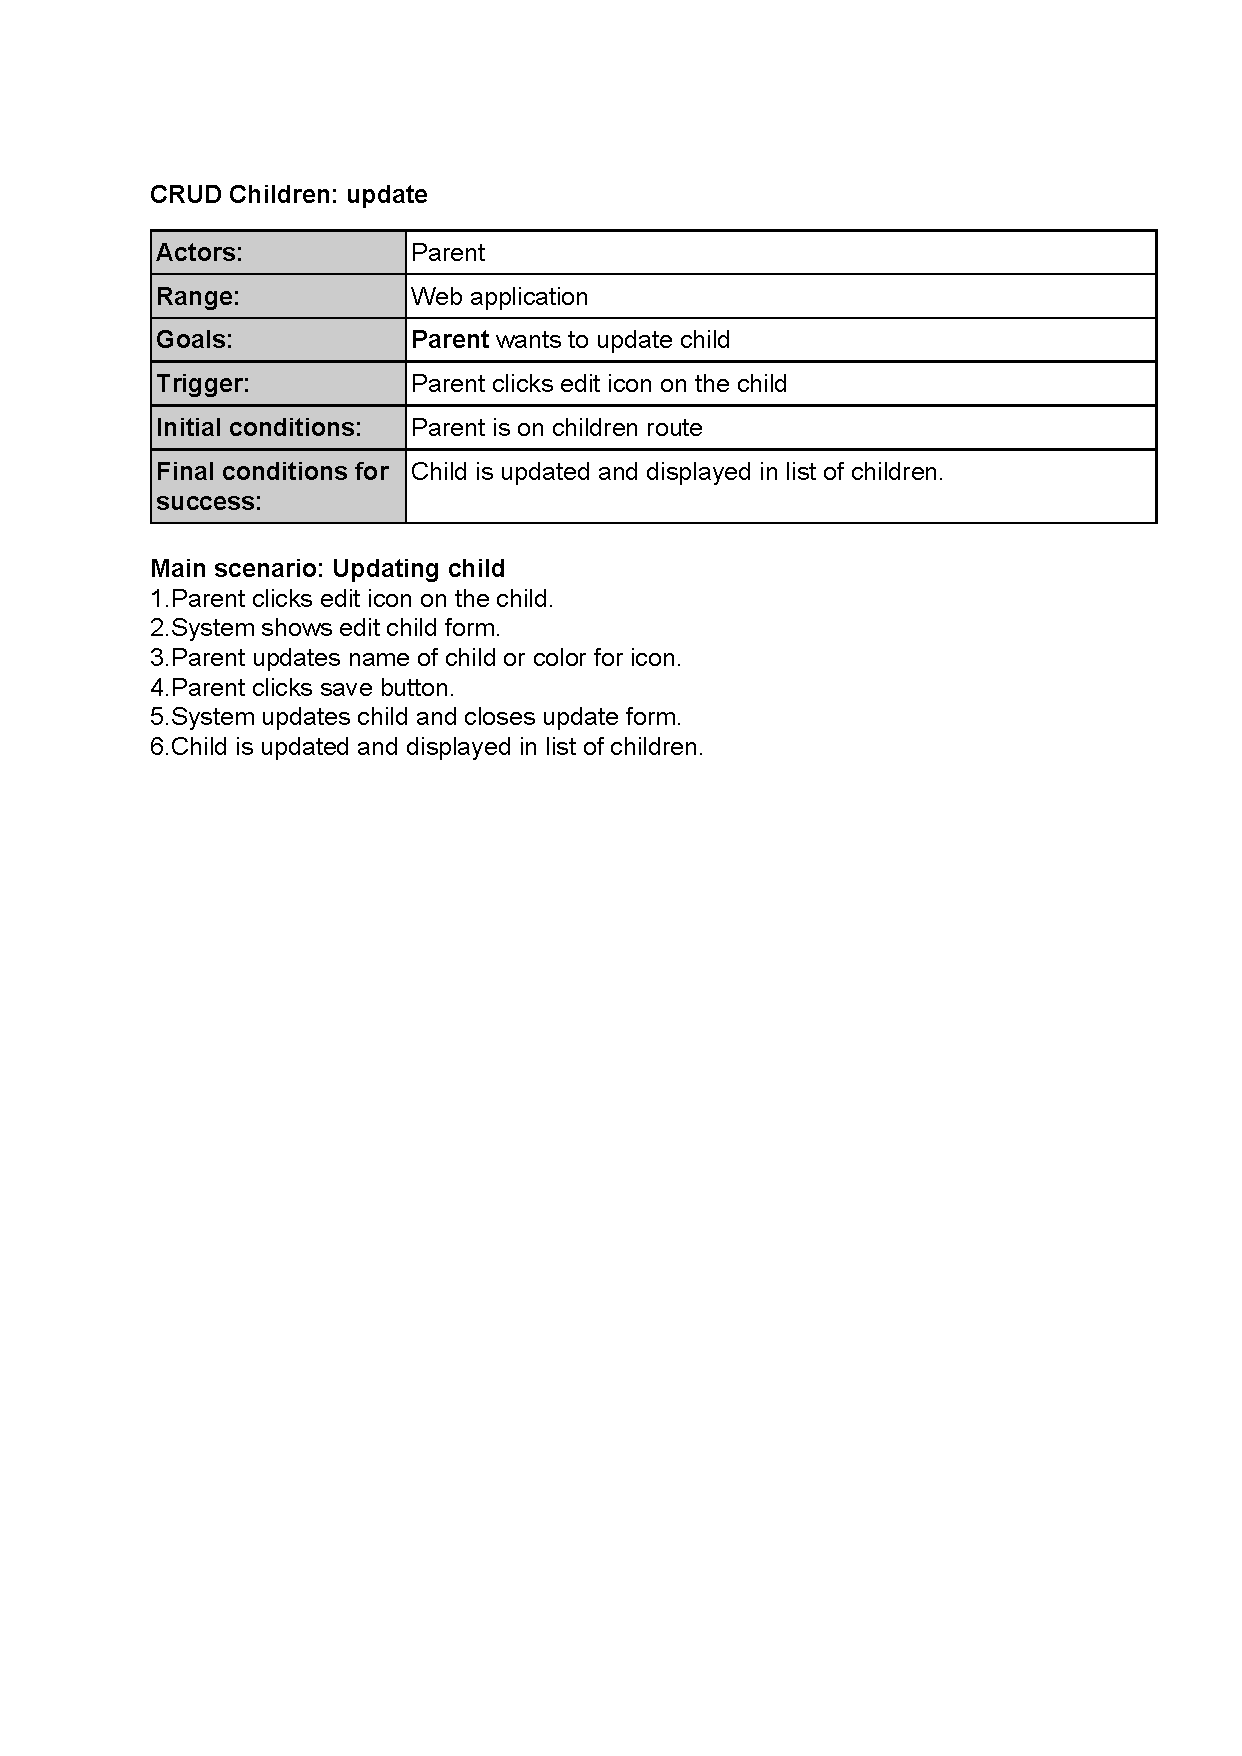
\includegraphics[width=.80\textwidth]{upC_cropped} 
			\end{tabular} 
		\caption{Updating child scenario}
		\end{figure}

		\begin{figure}[H]
			\centering
			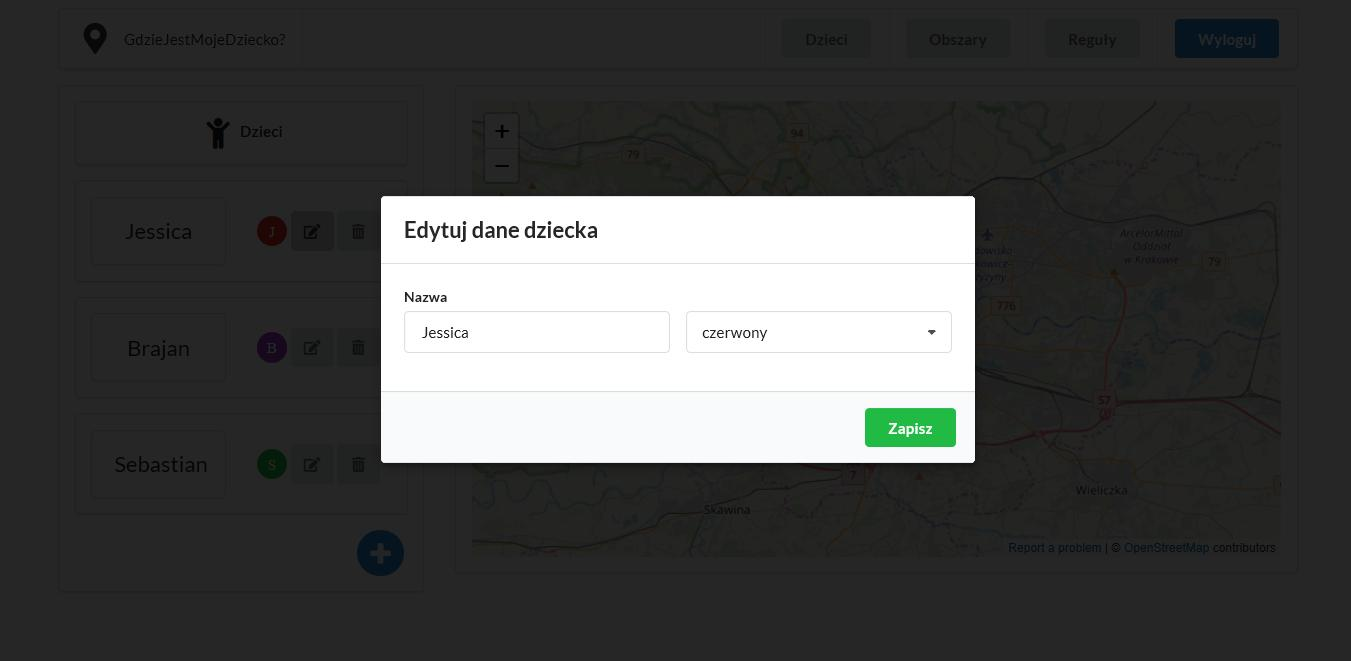
\includegraphics[width=.80\textwidth]{editChild}
			\caption{Editing child data}
		\end{figure}

		\begin{figure}[H] 
			\centering
			\begin{tabular}{c}
				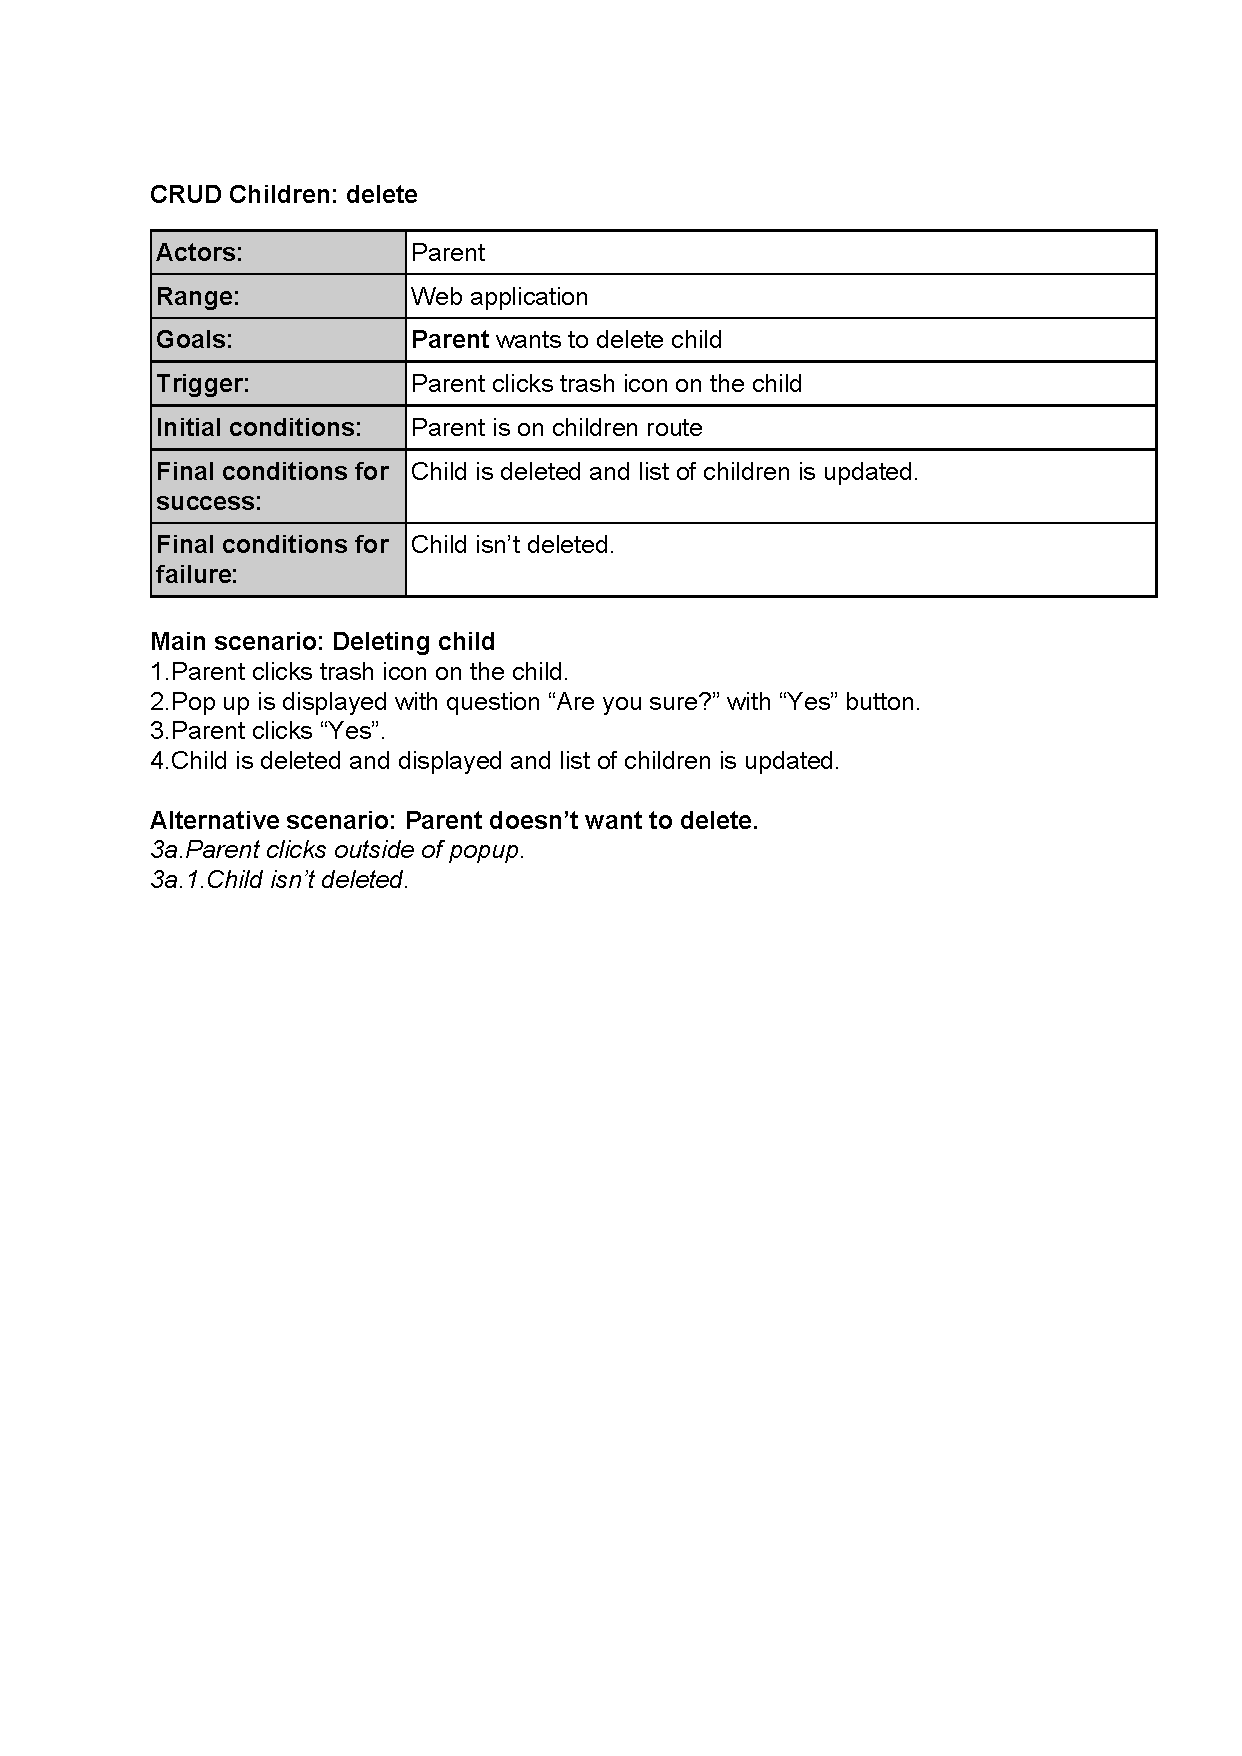
\includegraphics[width=.80\textwidth]{deC_cropped} 
			\end{tabular} 
		\caption{Deleting child scenario}
		\end{figure}

		\begin{figure}[H]
			\centering
			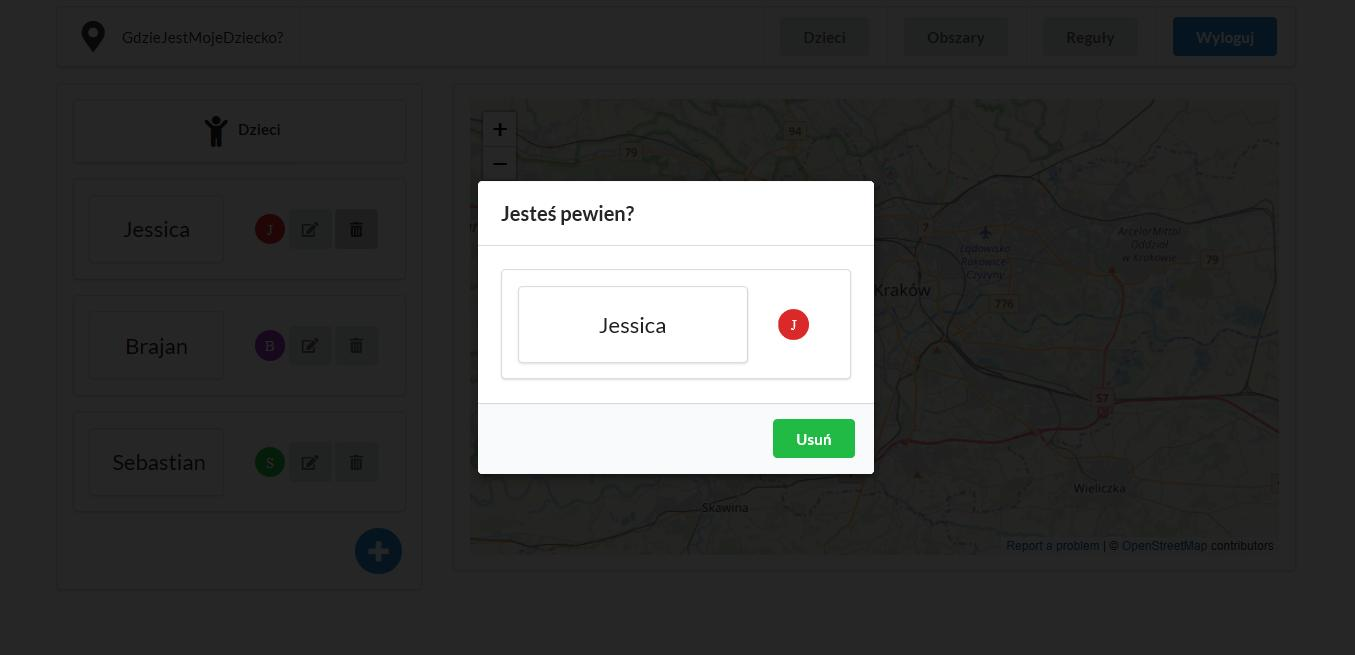
\includegraphics[width=.80\textwidth]{deleteChild}
			\caption{Deleting child}
		\end{figure}

		\begin{figure}[H]
			\centering
			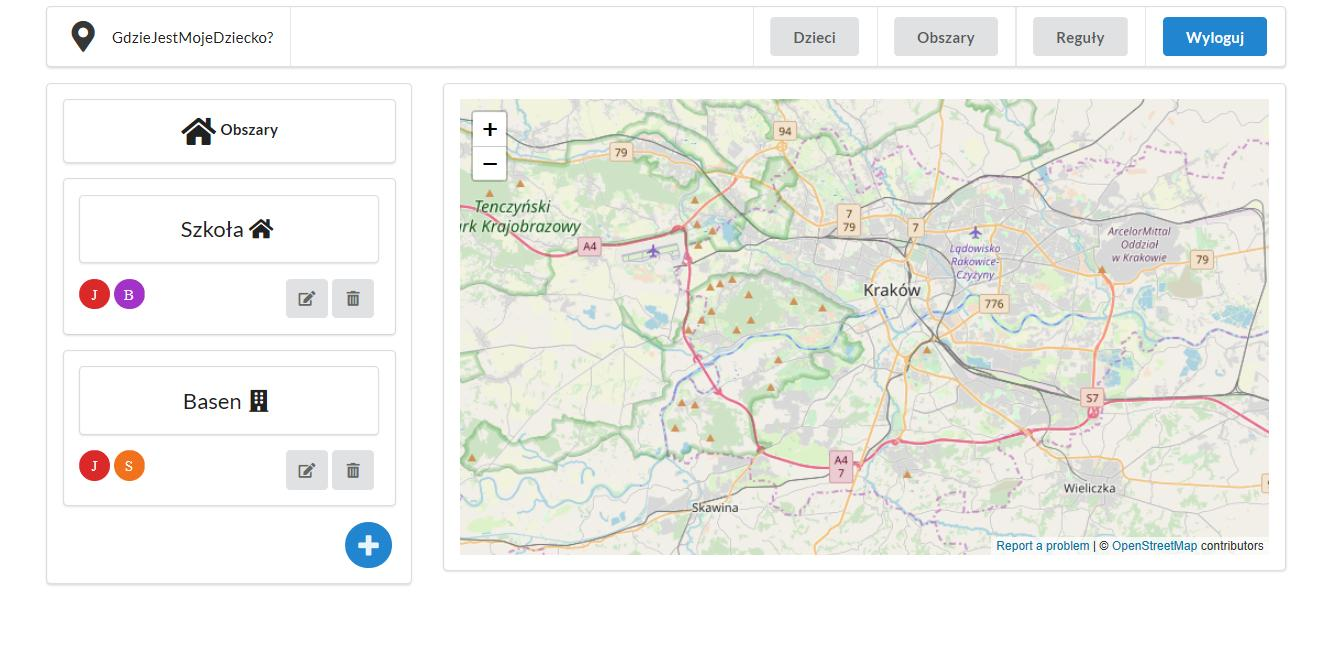
\includegraphics[width=.80\textwidth]{areas}
			\caption{Areas}
		\end{figure}

		\begin{figure}[H] 
			\centering
			\begin{tabular}{c}
				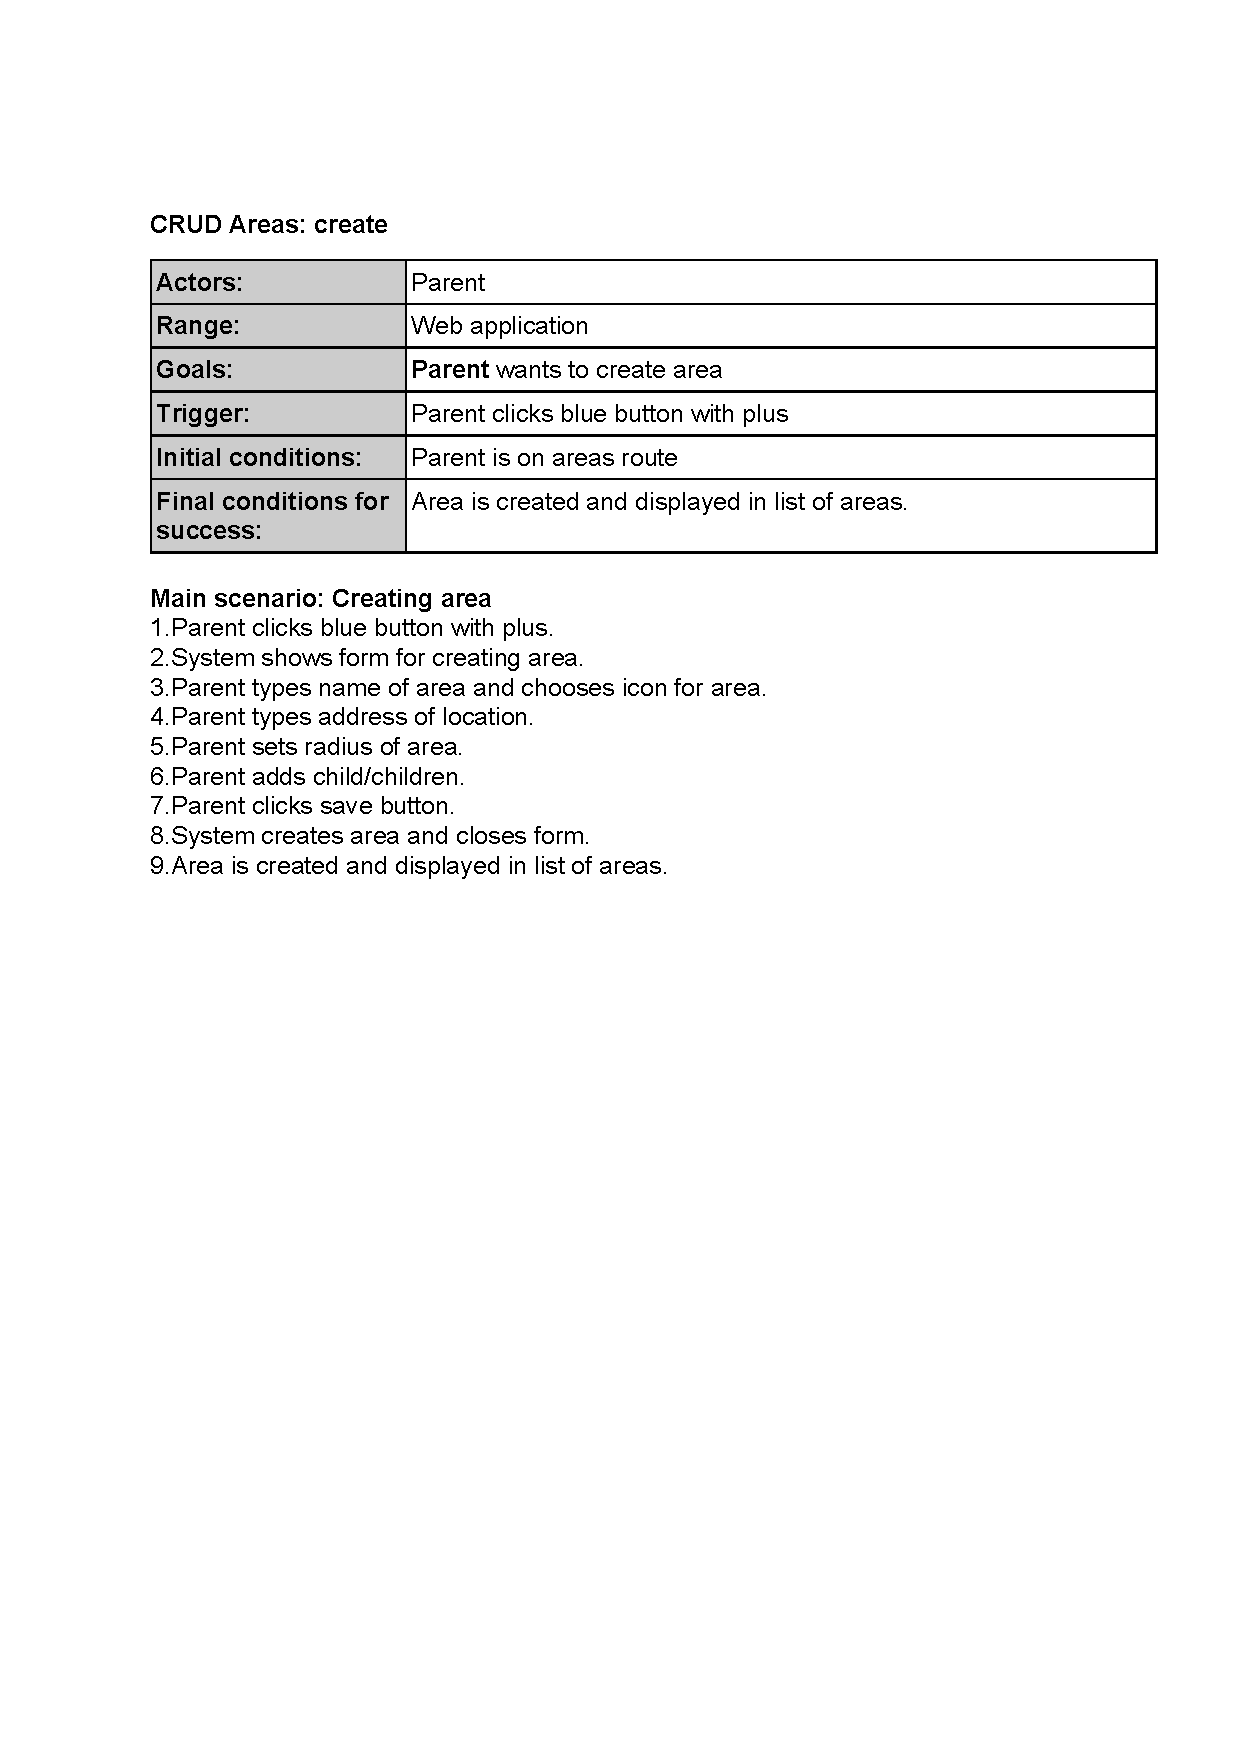
\includegraphics[width=.80\textwidth]{crA_cropped} 
			\end{tabular} 
		\caption{Creating area scenario}
		\end{figure}

		\begin{figure}[H]
			\centering
			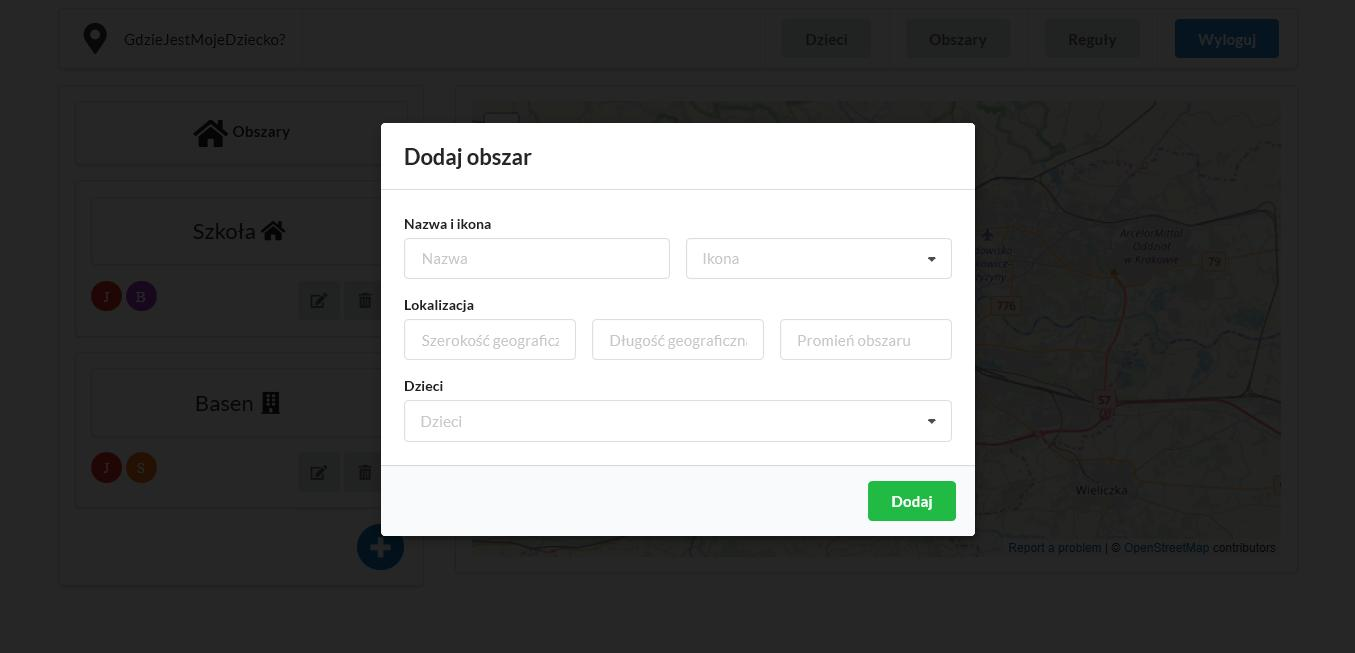
\includegraphics[width=.80\textwidth]{addArea}
			\caption{Creating area}
		\end{figure}

		\begin{figure}[H] 
			\centering
			\begin{tabular}{c}
				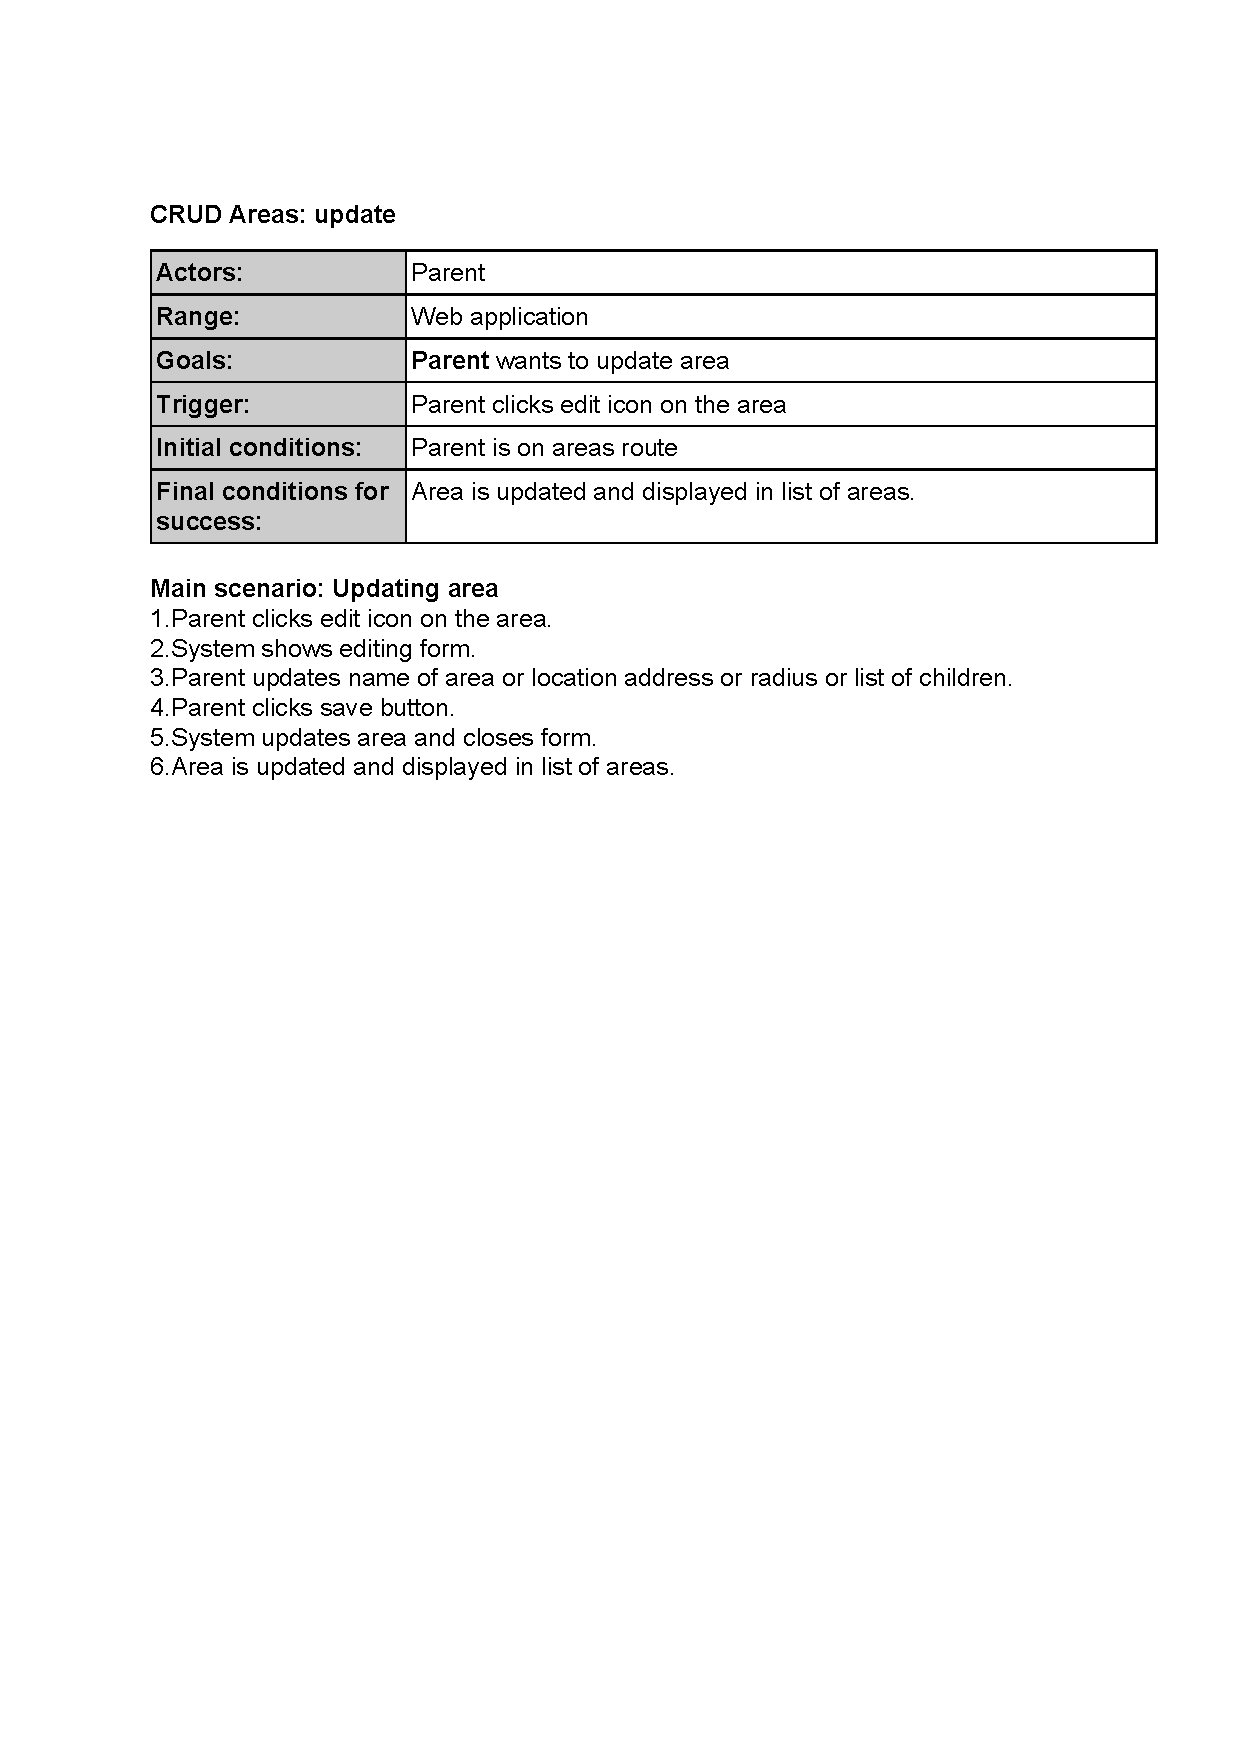
\includegraphics[width=.80\textwidth]{upA_cropped} 
			\end{tabular} 
		\caption{Updating area scenario}
		\end{figure}

		\begin{figure}[H]
			\centering
			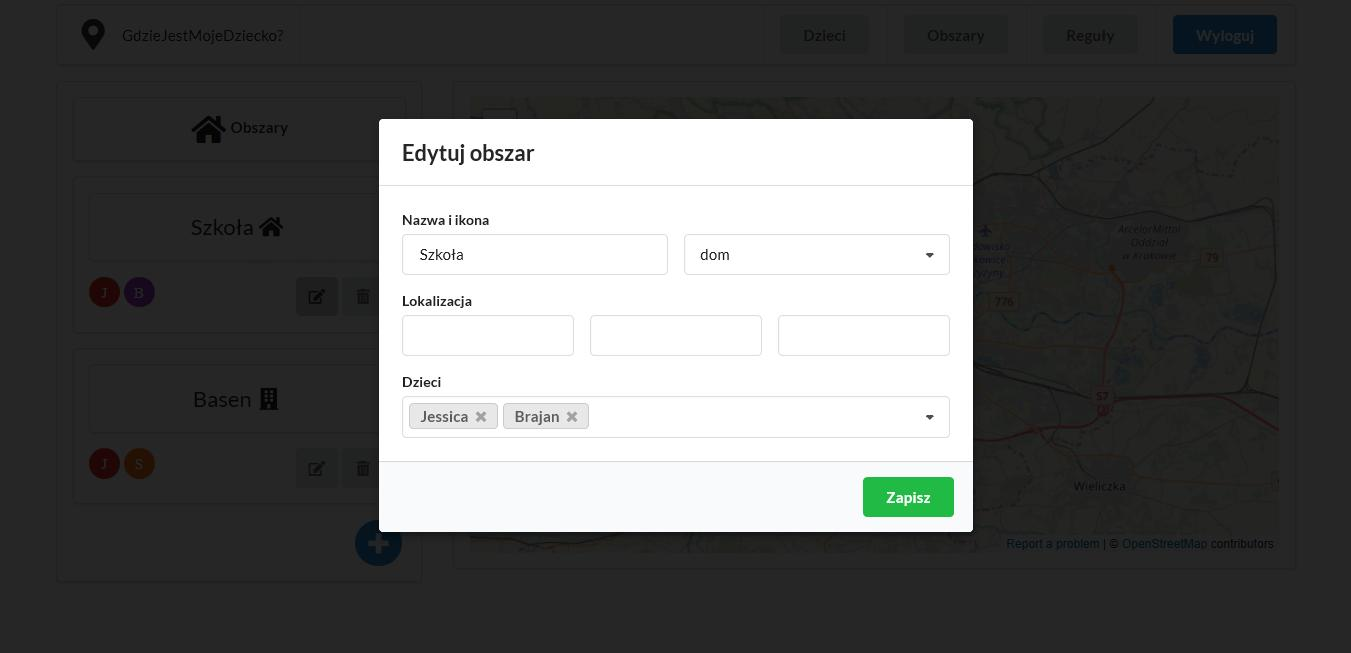
\includegraphics[width=.80\textwidth]{editArea}
			\caption{Editing area}
		\end{figure}

		\begin{figure}[H] 
			\centering
			\begin{tabular}{c}
				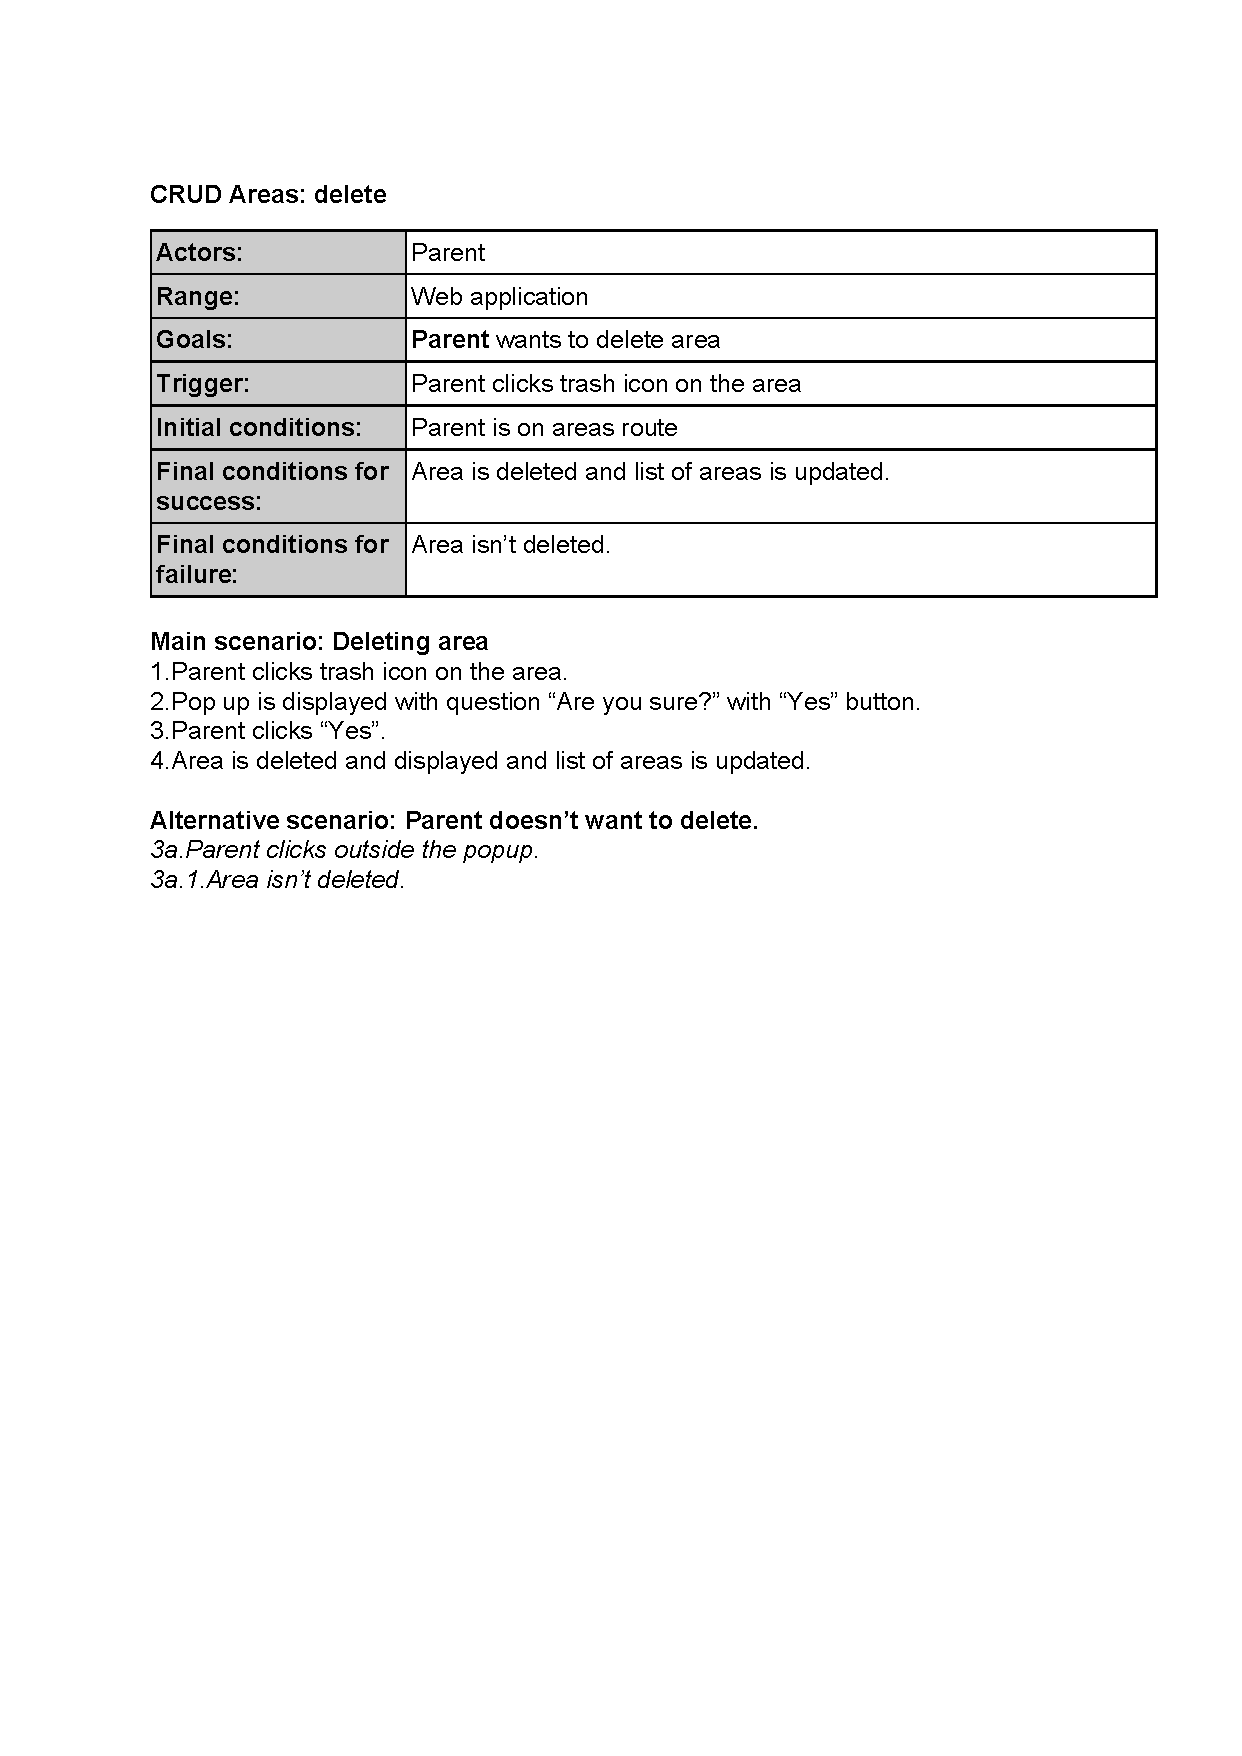
\includegraphics[width=.80\textwidth]{deA_cropped} 
			\end{tabular} 
		\caption{Deleting area scenario}
		\end{figure}

		\begin{figure}[H]
			\centering
			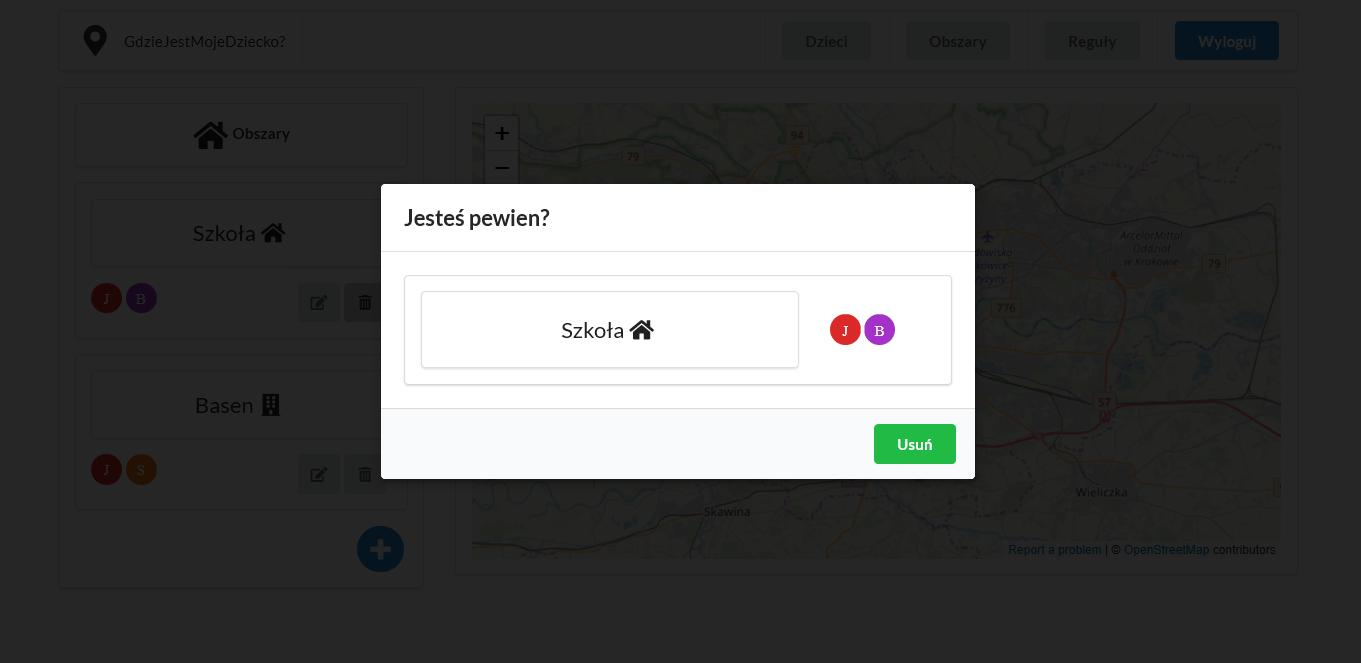
\includegraphics[width=.80\textwidth]{deleteArea}
			\caption{Deleting area}
		\end{figure}

		\begin{figure}[H]
			\centering
			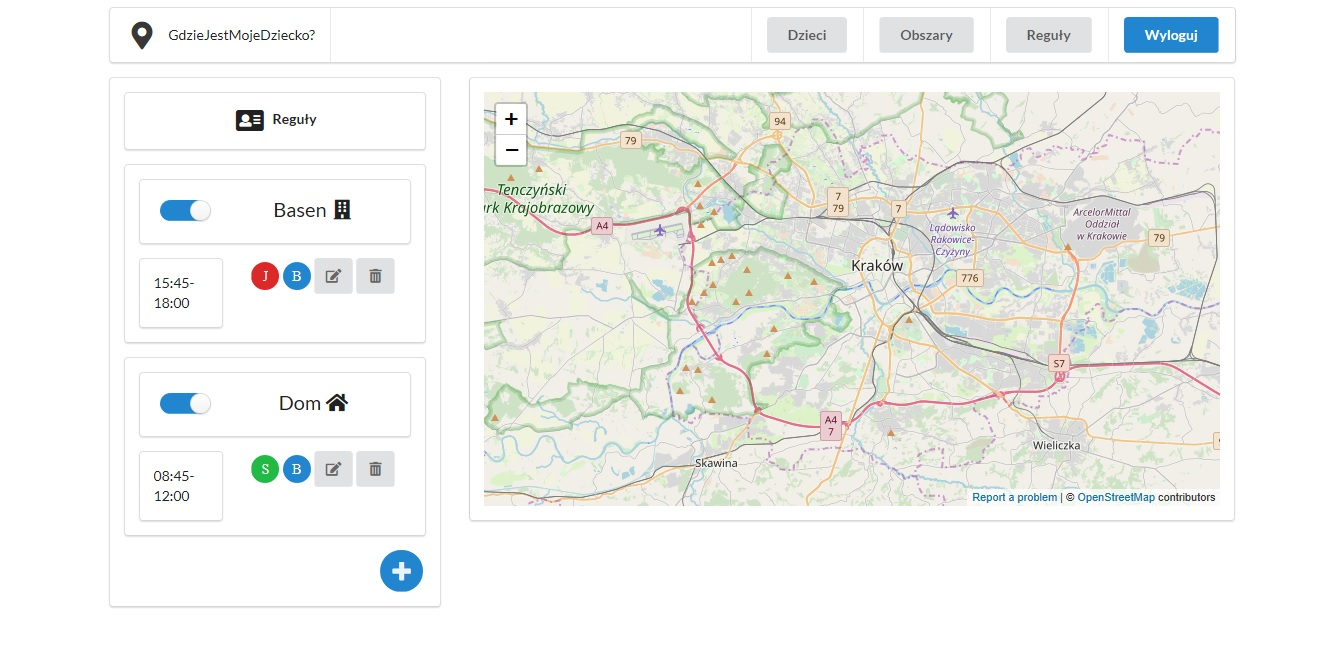
\includegraphics[width=.80\textwidth]{rules}
			\caption{Rules}
		\end{figure}

		\begin{figure}[H] 
			\centering
			\begin{tabular}{c}
				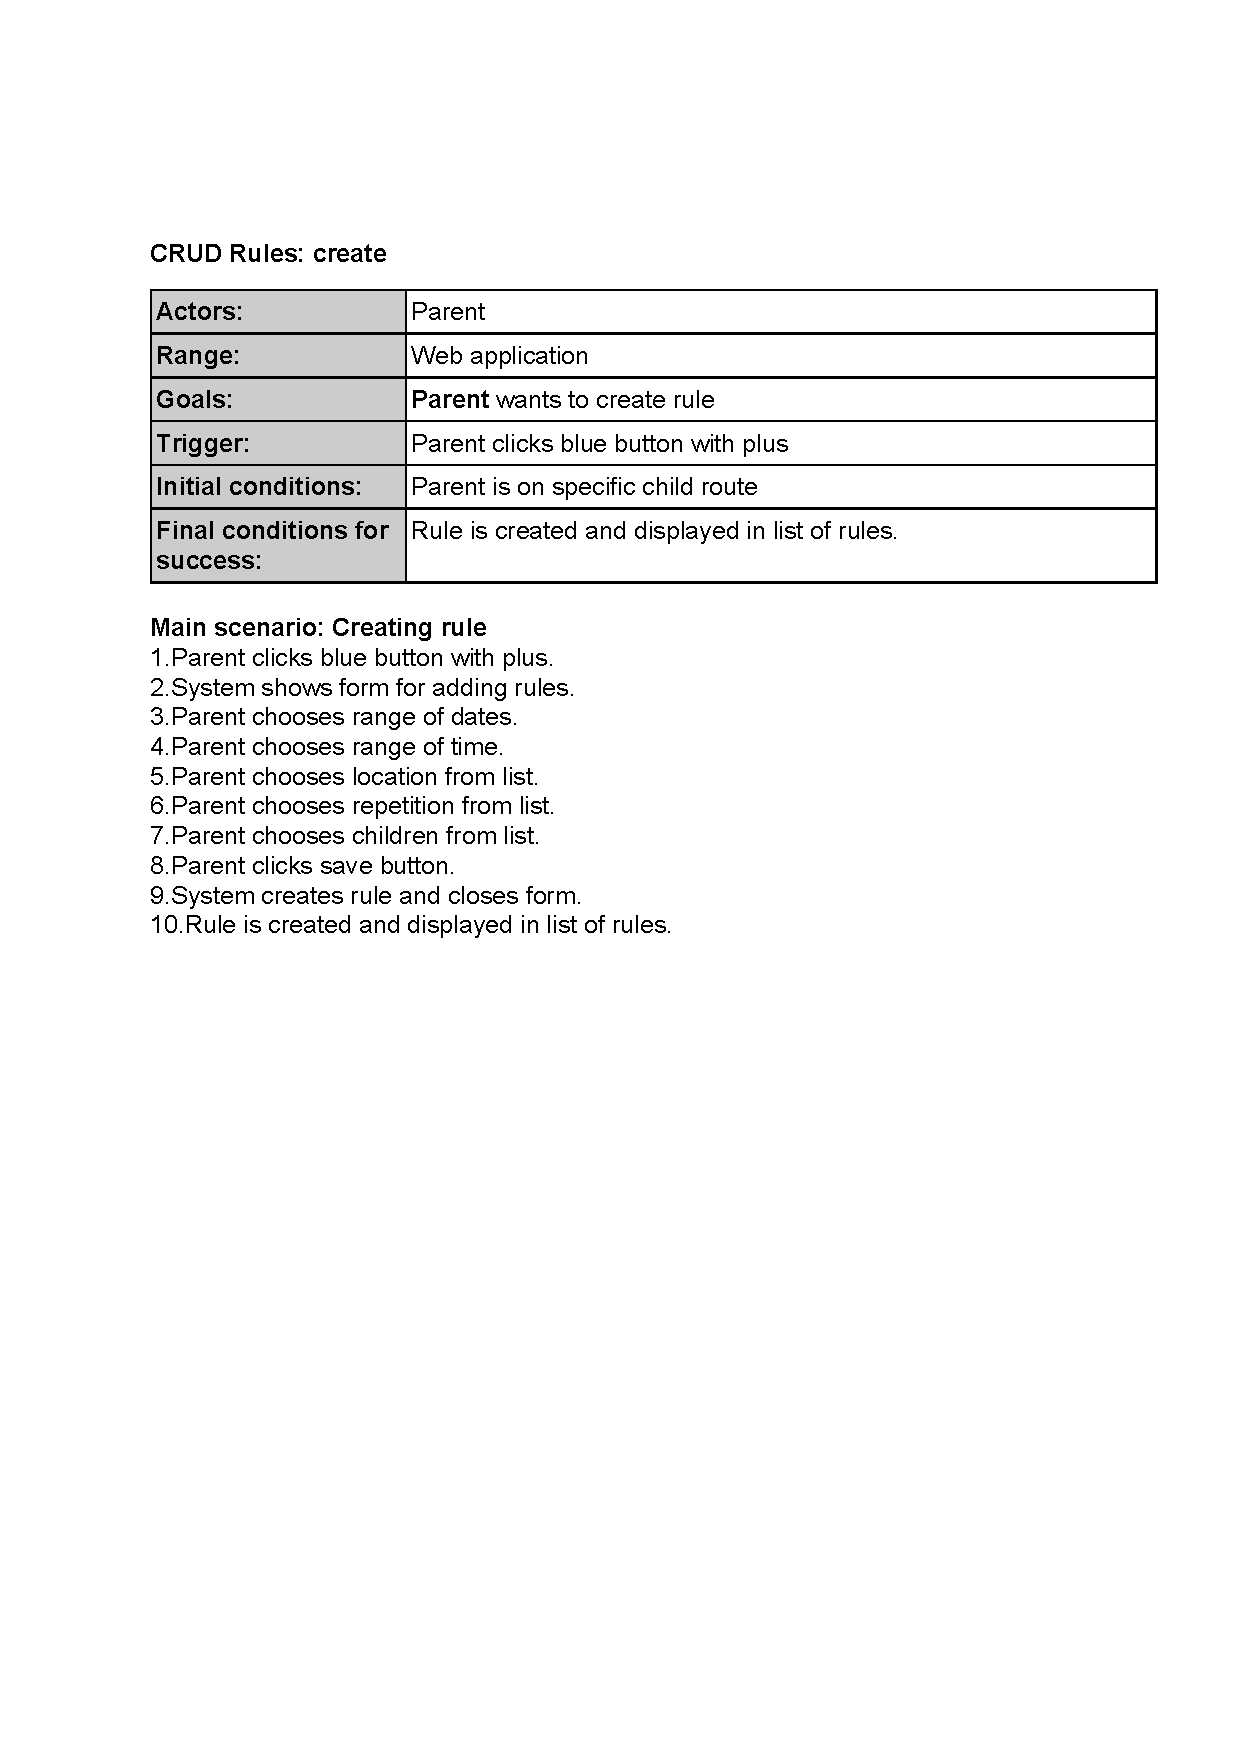
\includegraphics[width=.80\textwidth]{crR_cropped} 
			\end{tabular} 
		\caption{Creating rule scenario}
		\end{figure}

		\begin{figure}[H]
			\centering
			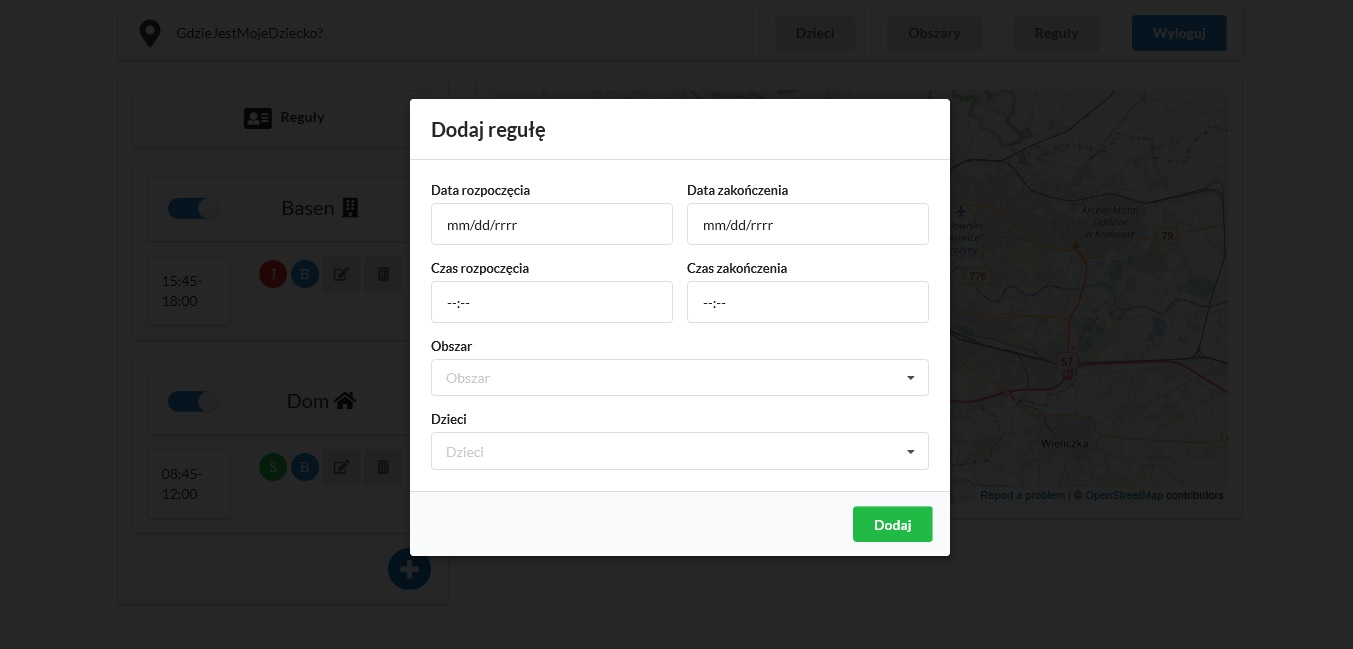
\includegraphics[width=.80\textwidth]{addRule}
			\caption{Creating rule}
		\end{figure}

		\begin{figure}[H] 
			\centering
			\begin{tabular}{c}
				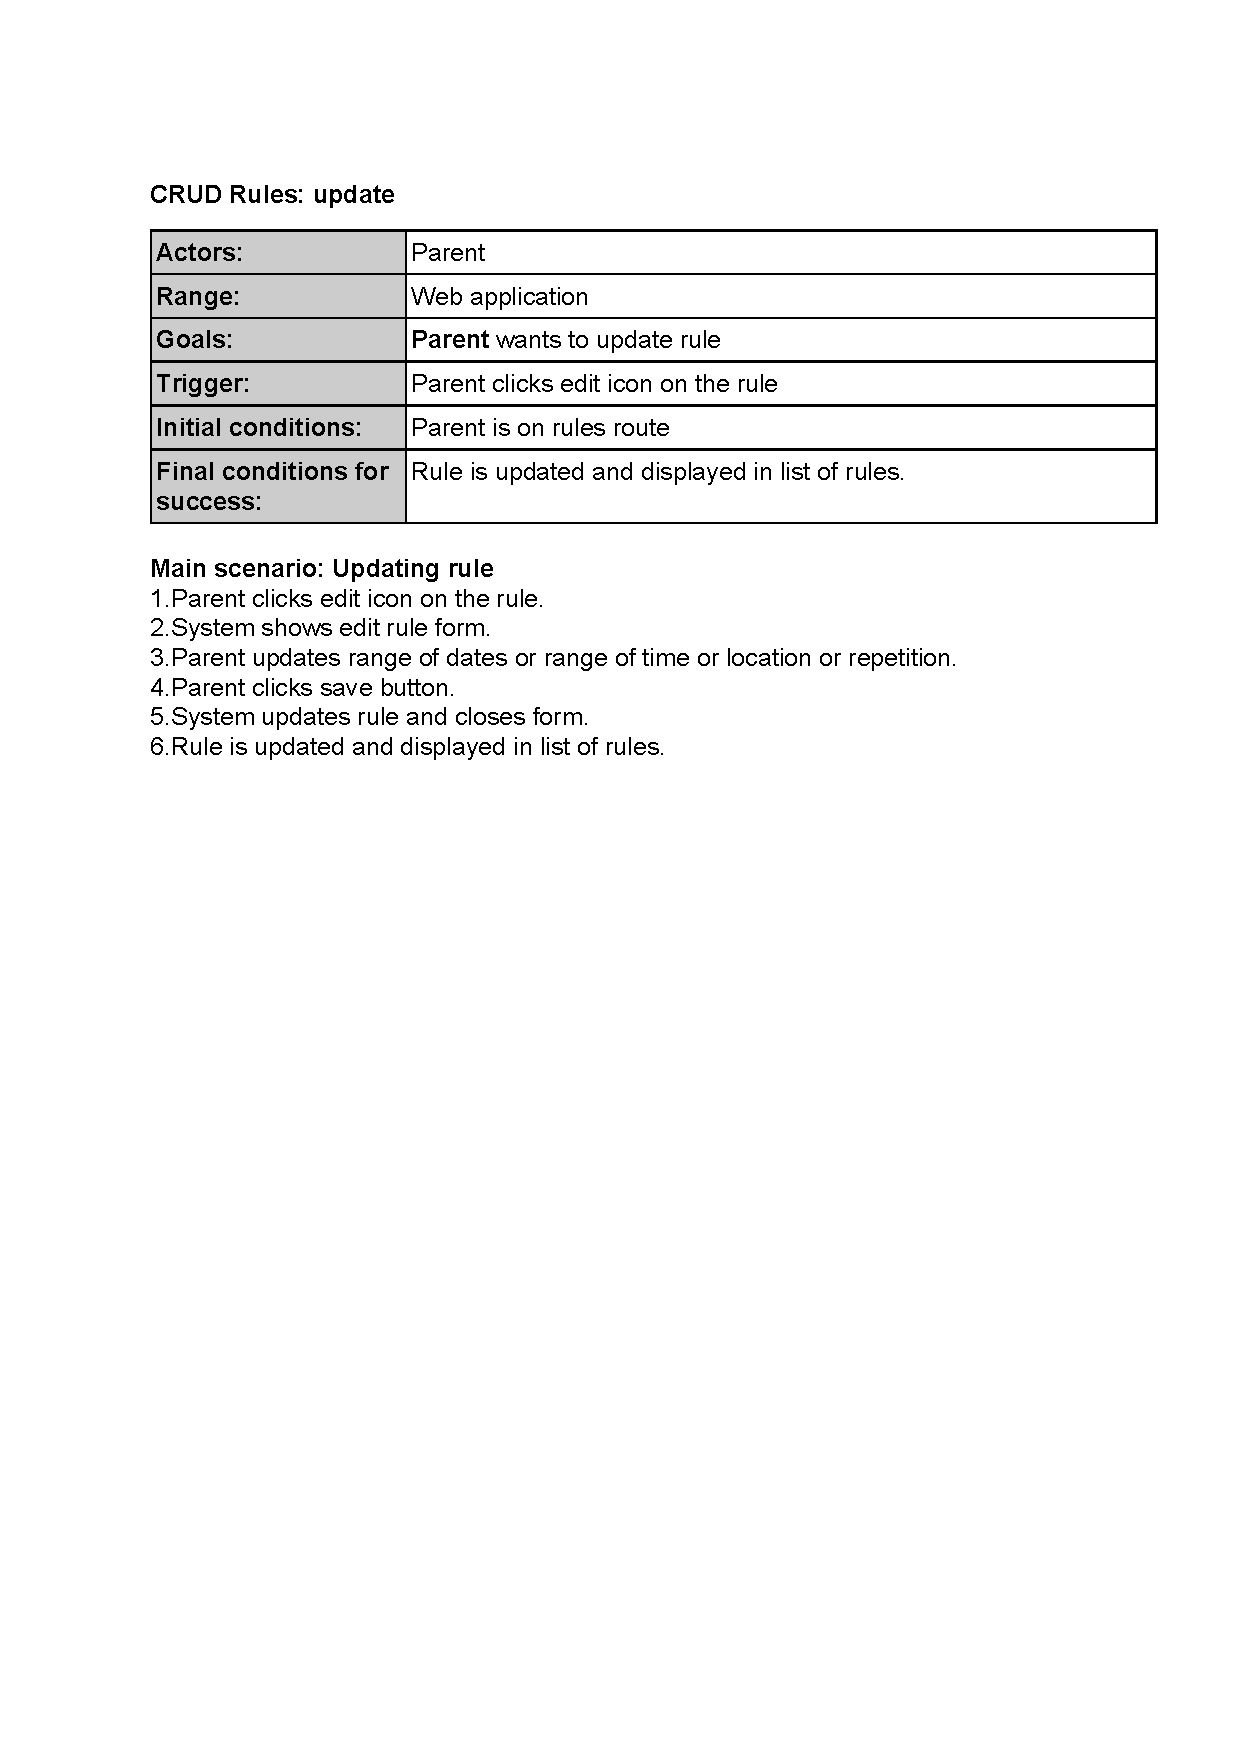
\includegraphics[width=.80\textwidth]{upR_cropped} 
			\end{tabular} 
		\caption{Updating rule scenario}
		\end{figure}

		\begin{figure}[H]
			\centering
			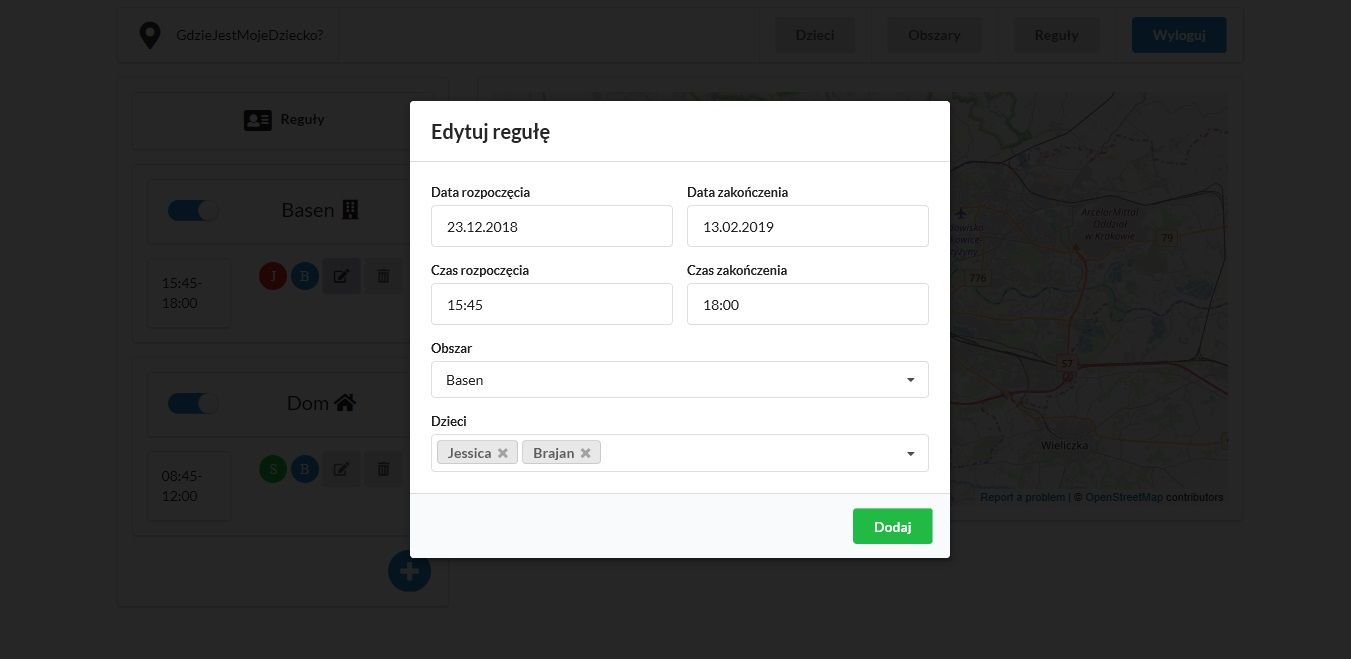
\includegraphics[width=.80\textwidth]{editRule}
			\caption{Updating rule}
		\end{figure}

		\begin{figure}[H] 
			\centering
			\begin{tabular}{c}
				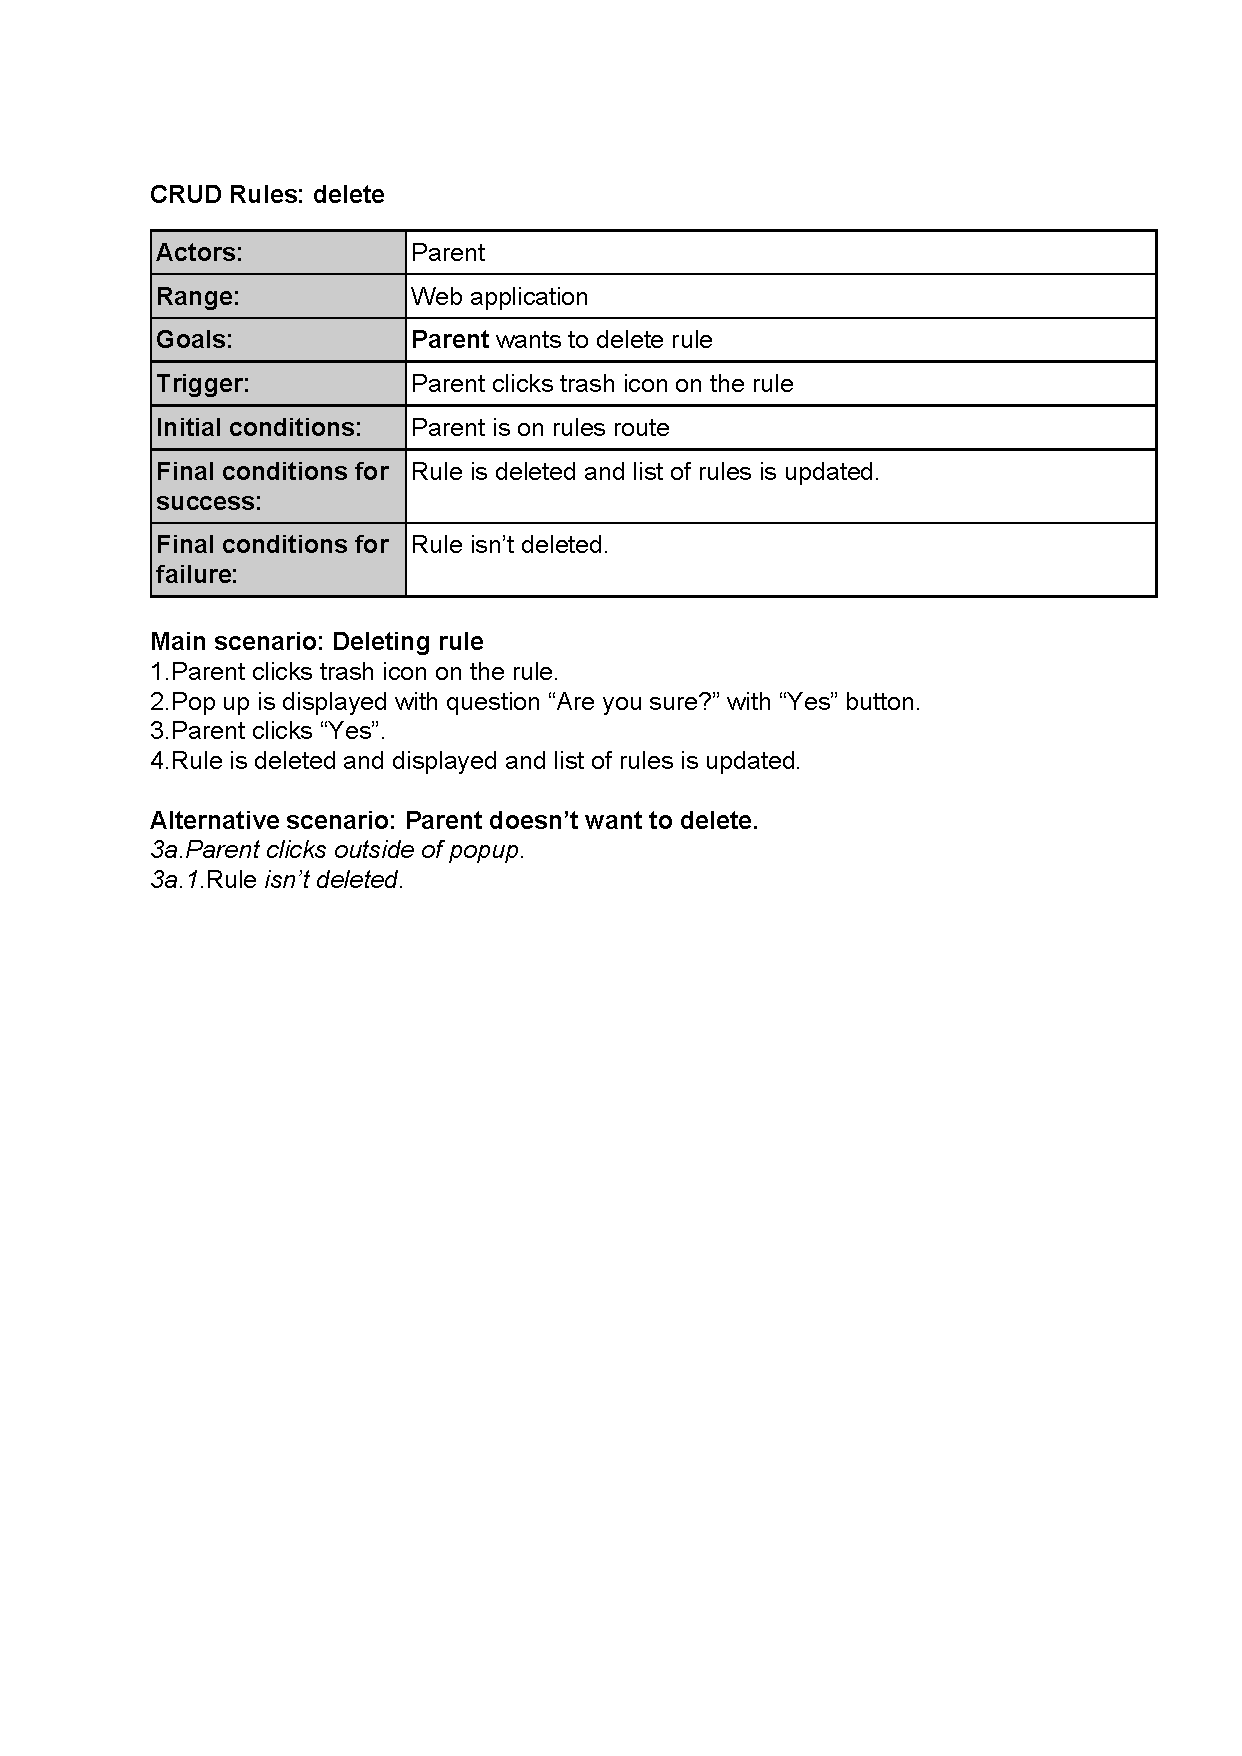
\includegraphics[width=.80\textwidth]{deR_cropped} 
			\end{tabular}  
		\caption{Deleting rule scenario}
		\end{figure}

		\begin{figure}[H]
			\centering
			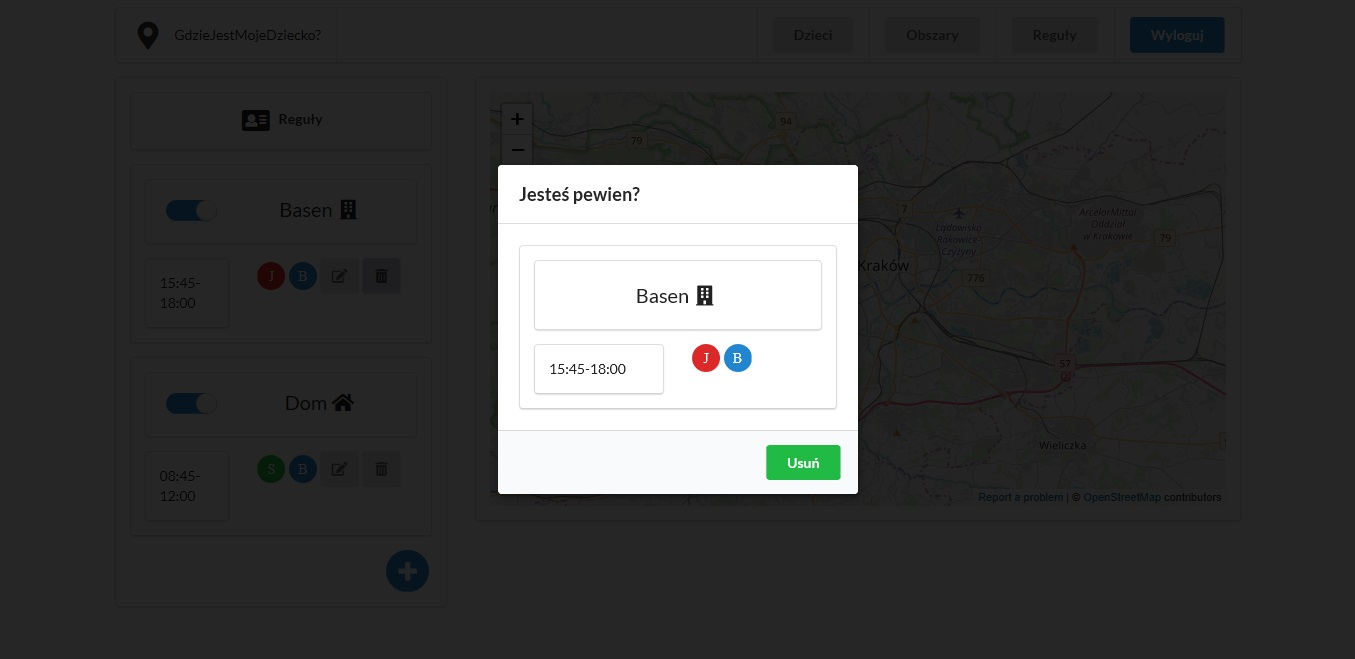
\includegraphics[width=.80\textwidth]{deleteRule}
			\caption{Deleting rule}
		\end{figure}

		\begin{figure}[H] 
			\centering
			\begin{tabular}{c}
				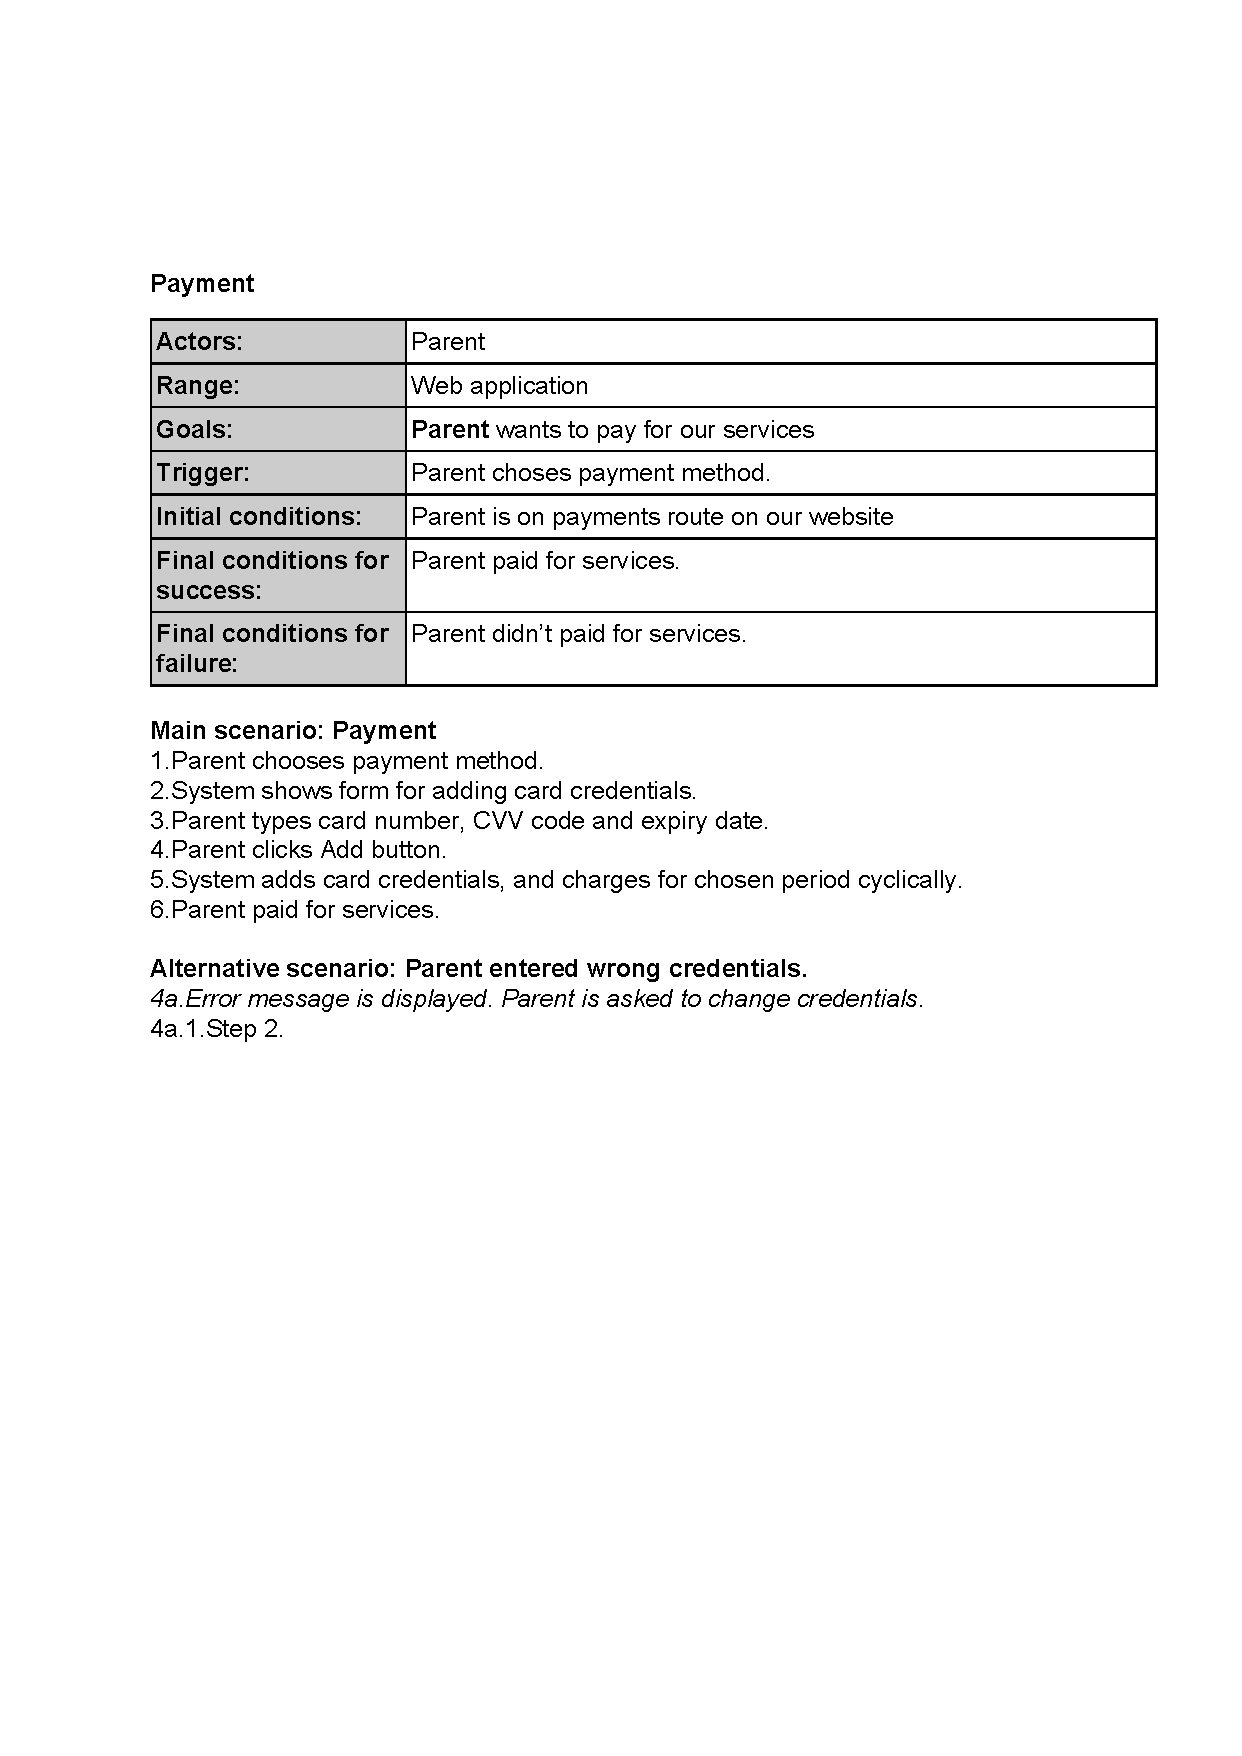
\includegraphics[width=.80\textwidth]{pay_cropped} 
			\end{tabular}  
		\caption{Payment scenario}
		\end{figure}

	\section{System's architecture}
		In our application we are using MongoDB, so our database is identical to our class diagram.
		
		\begin{figure}[H] 
			\centering
			\begin{tabular}{c}
				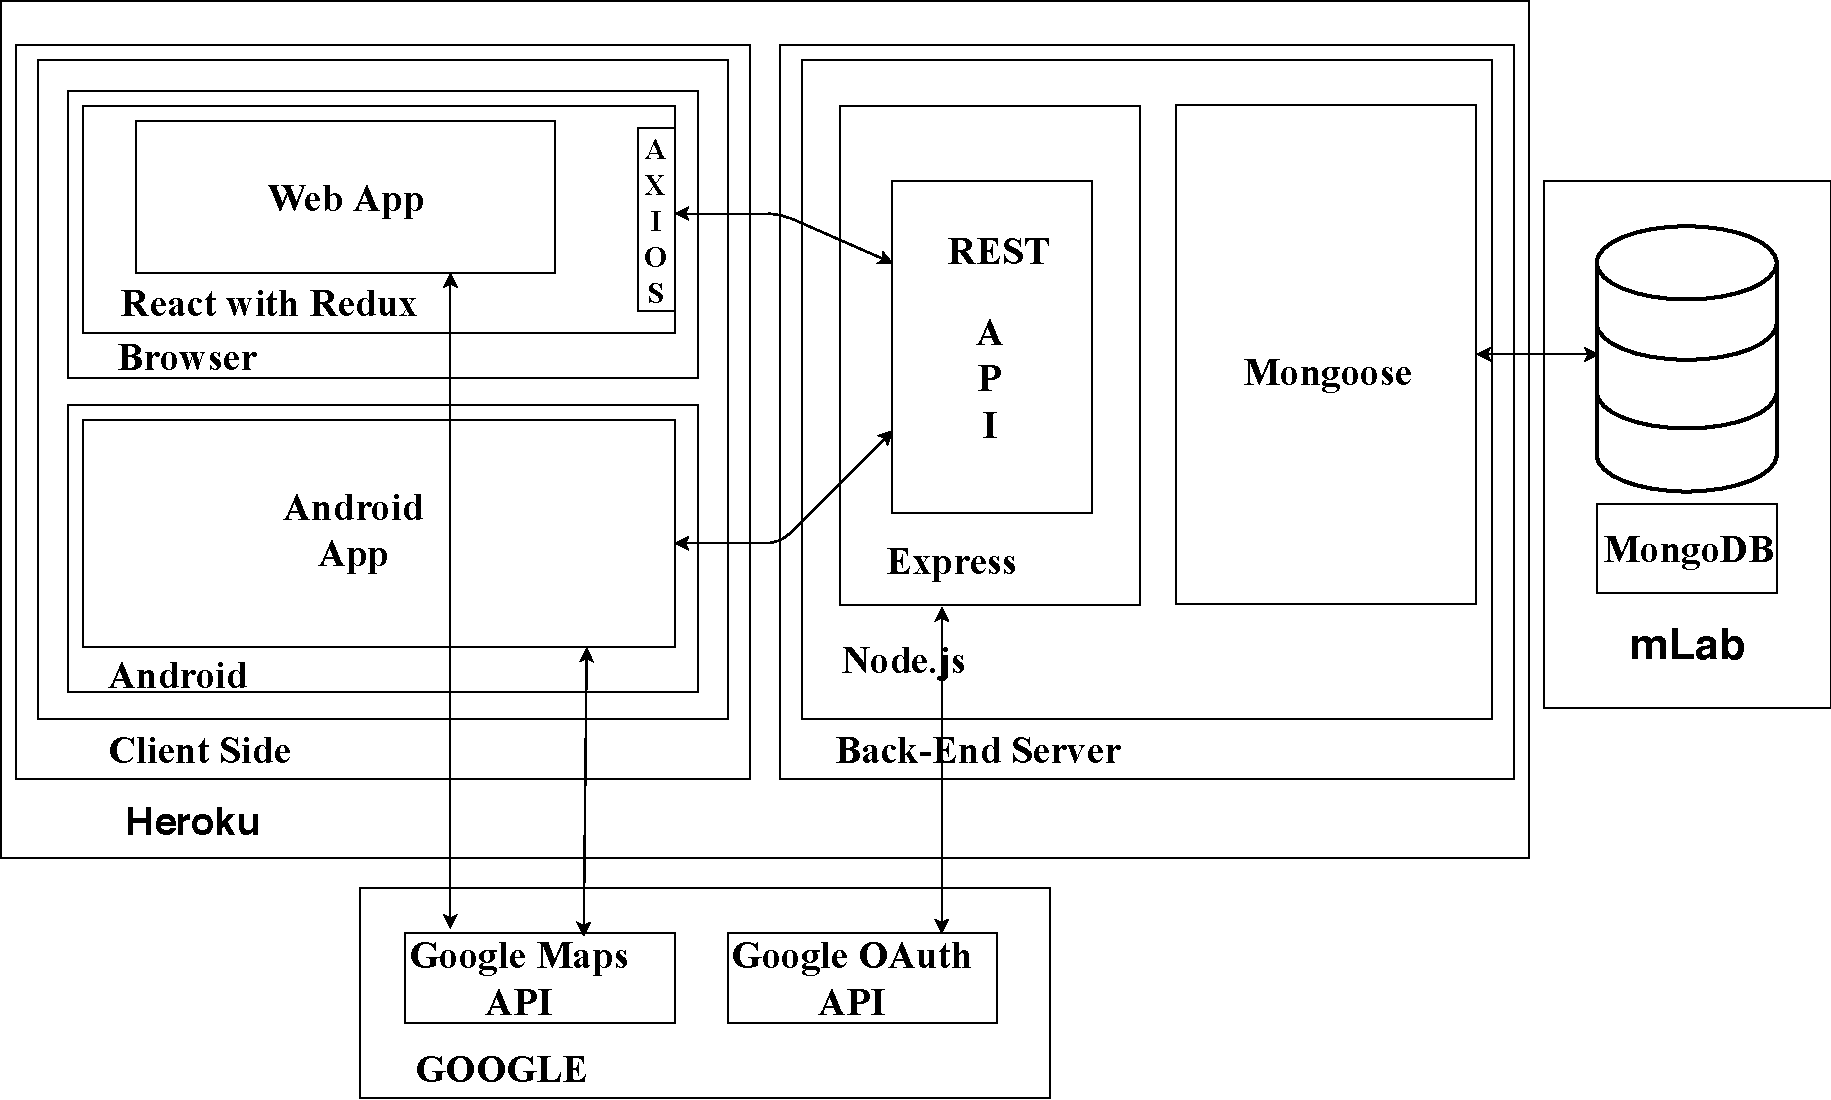
\includegraphics[width=.95\textwidth]{moduly_interfejsy_komunikacyjne}
			\end{tabular} 
			\caption{Architecture, modules and interfaces}
		\end{figure}

		\subsection{Project of tests}
		
		\begin{table}[H]
			\centering
			\begin{tabular}{|c|c|c|}
				\hline
				\textbf{Tests} & \textbf{What?} & \textbf{Technologies} \\
				\hline
				Unit & backend and frontend methods & Jasmine \\ \hline
				Integration & communication between modules & Jasmine \\ \hline
				Functional & use cases & Jasmine, Selenium \\ \hline
				Manual & Mobile application & manually \\ \hline
				Manual & API & postman \\ \hline
			\end{tabular}
			\caption{Project of tests} 
		\end{table}

	\section{Project of software}

		\subsection{Client side: React Components}

			Platform: JavaScript -> JSX -> HTML

			\begin{figure}[H] 
				\centering
				\begin{tabular}{c}
					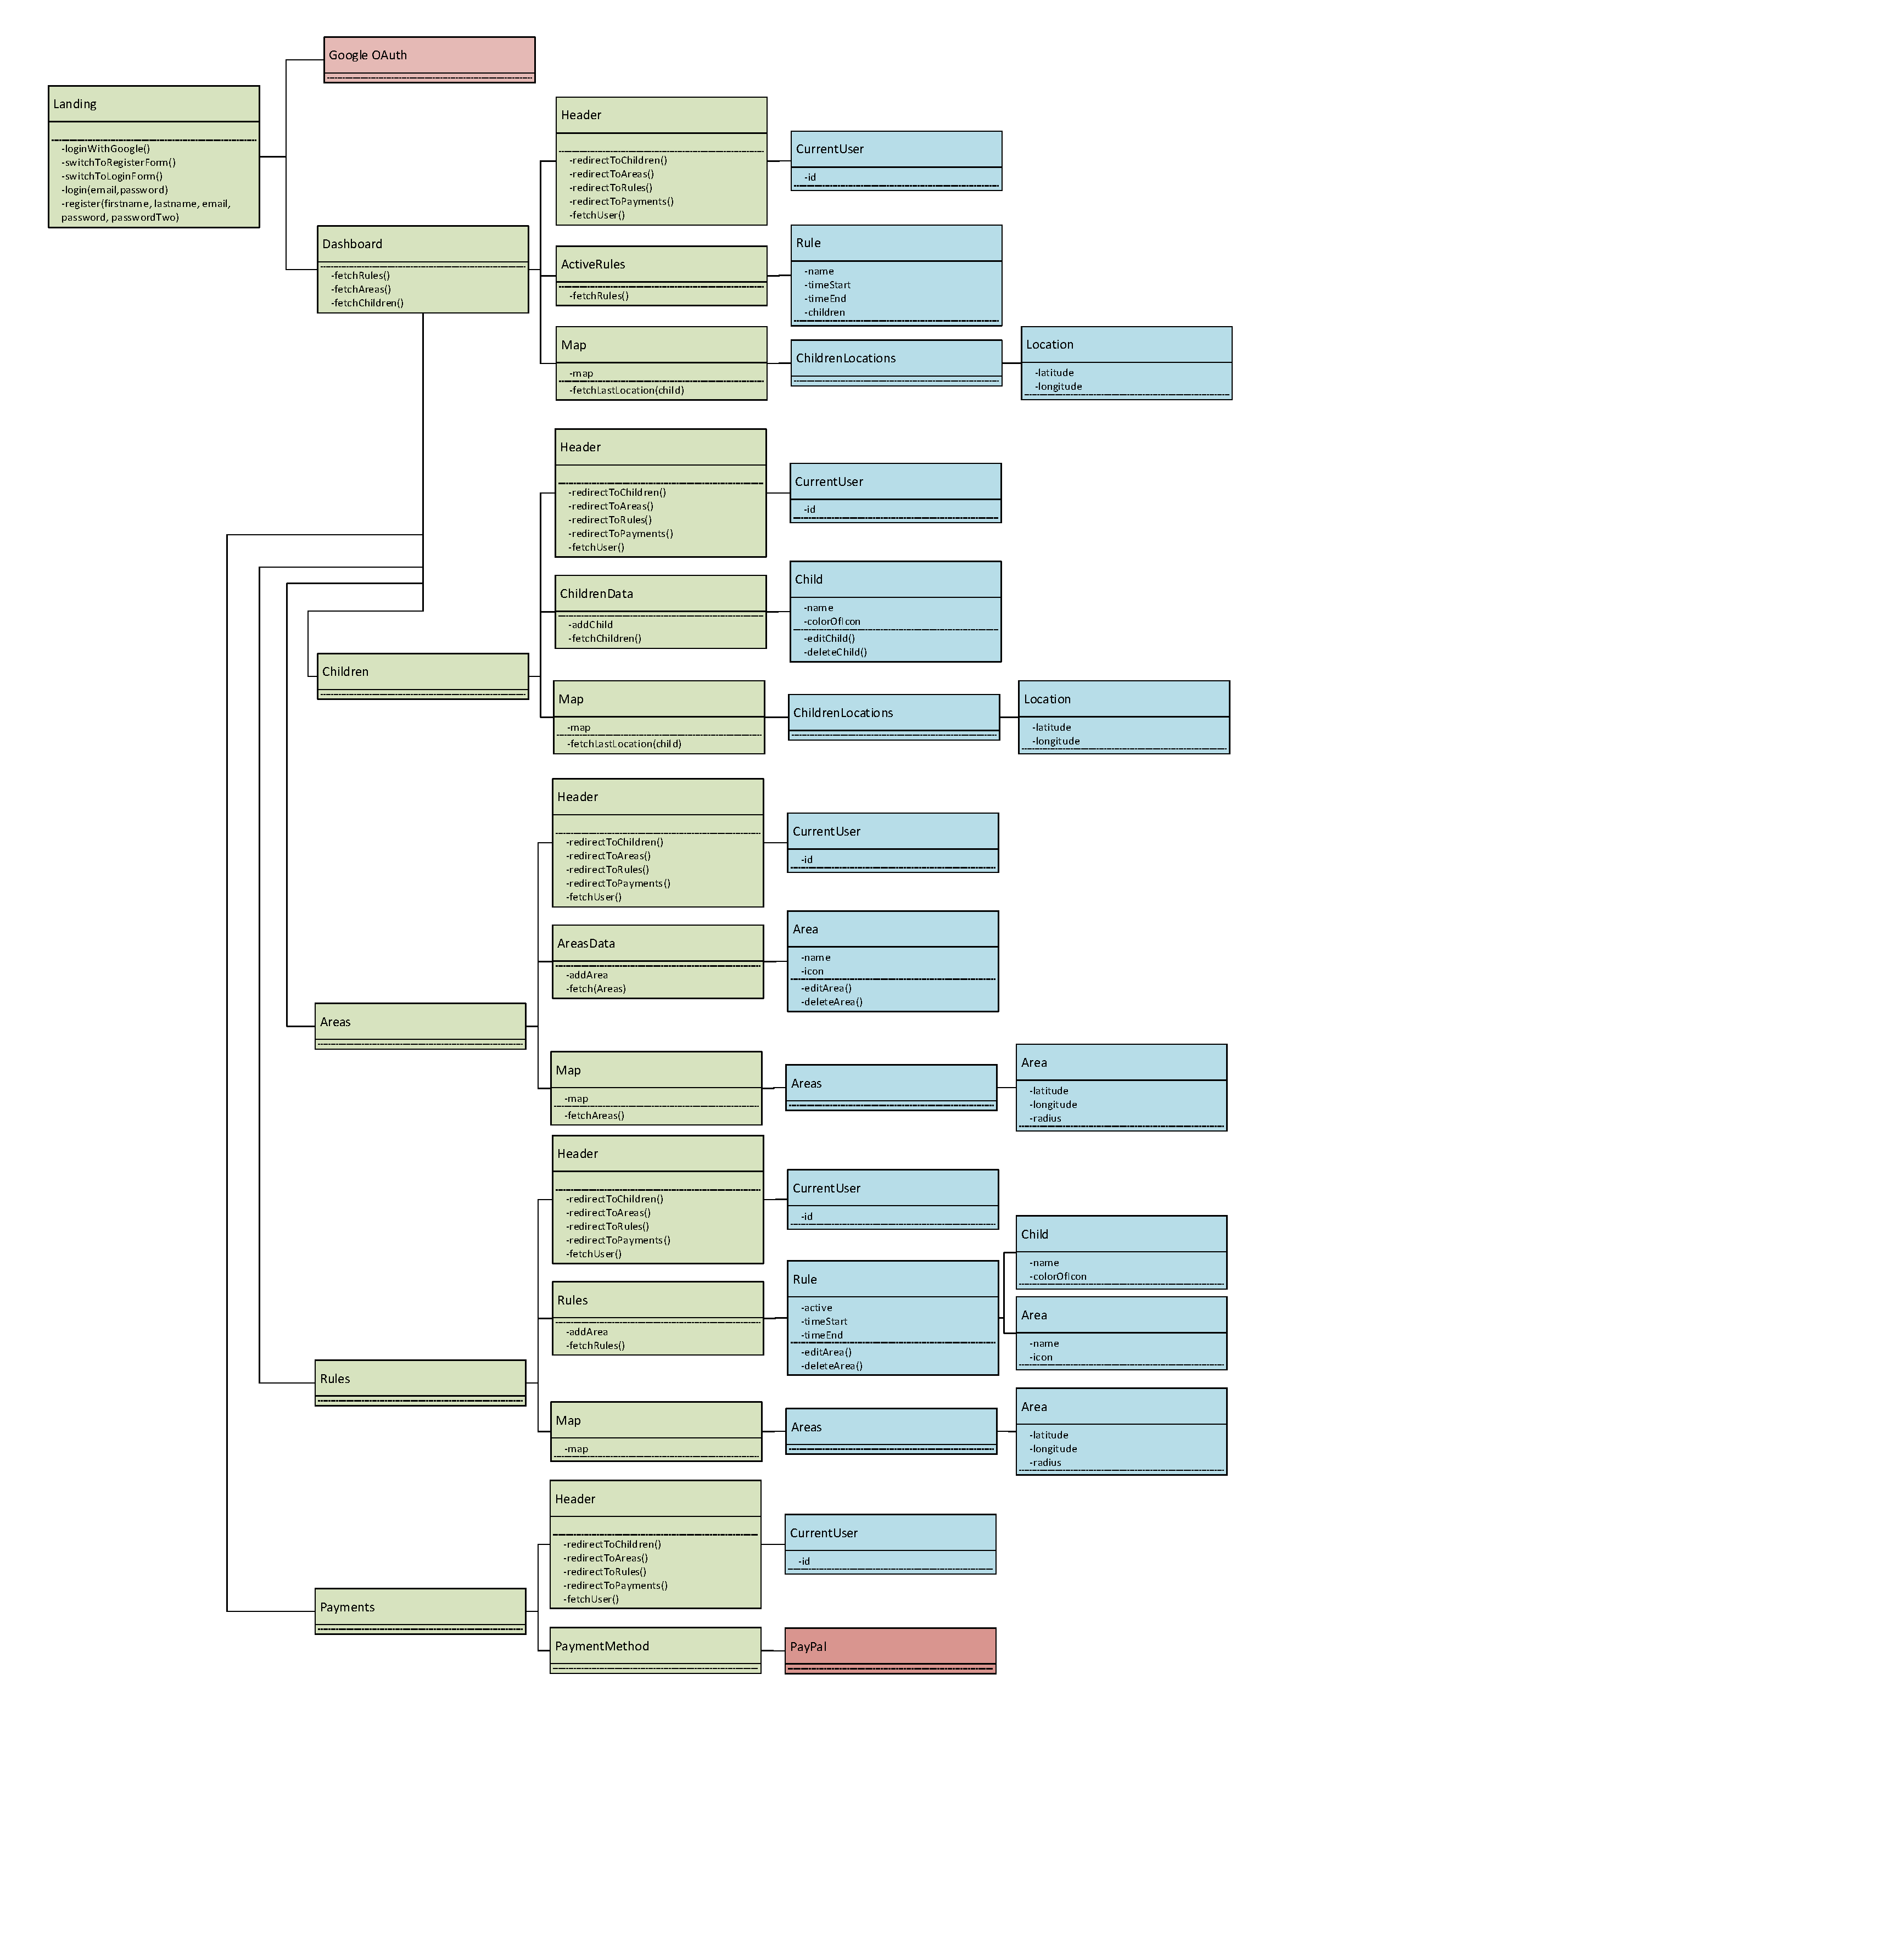
\includegraphics[width=.95\textwidth]{ProjektOprogramowania}
				\end{tabular} 
				\caption{Software project}
			\end{figure}
		
			\begin{figure}[H] 
				\centering
				\begin{tabular}{c}
					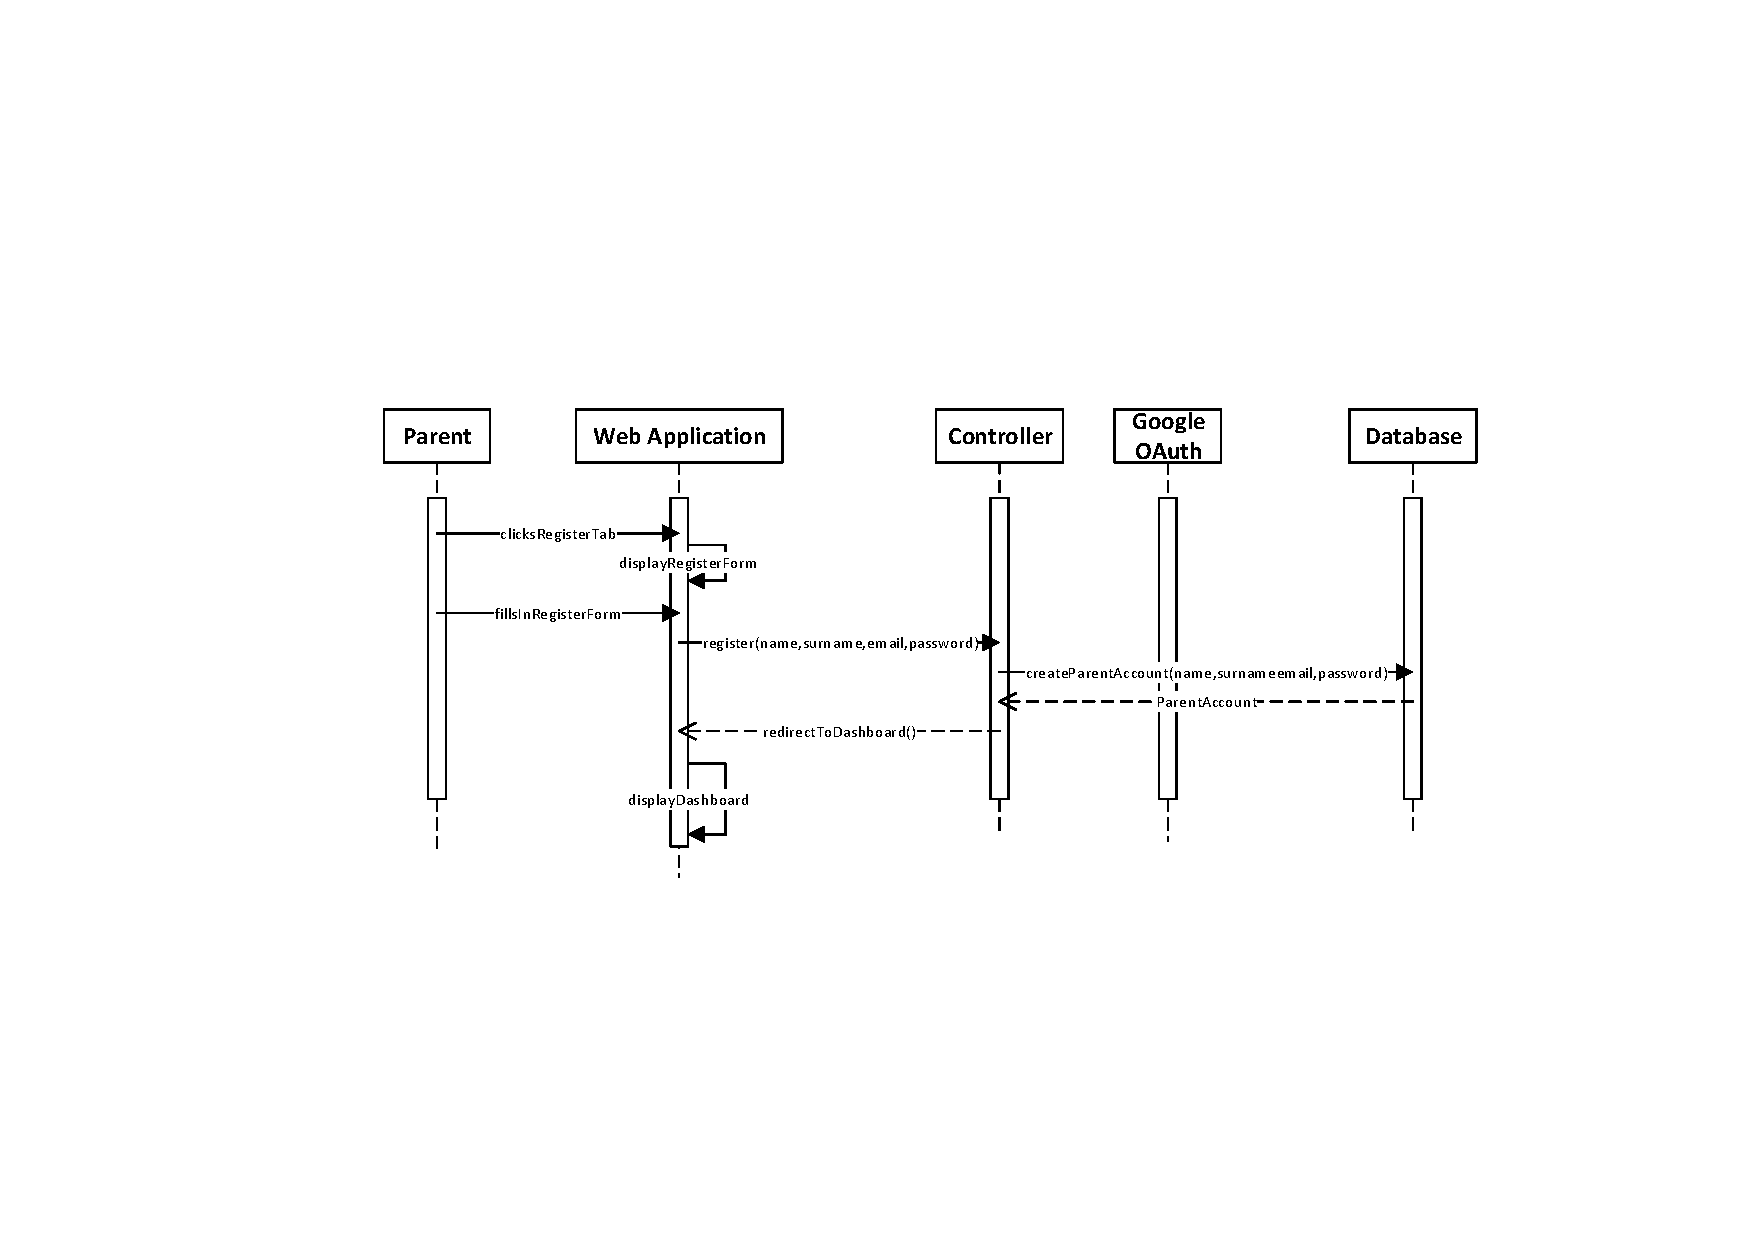
\includegraphics[width=.95\textwidth]{registerSequenceDiagram}
				\end{tabular} 
				\caption{Register Sequence Diagram}
			\end{figure}
		
			\begin{figure}[H] 
				\centering
				\begin{tabular}{c}
					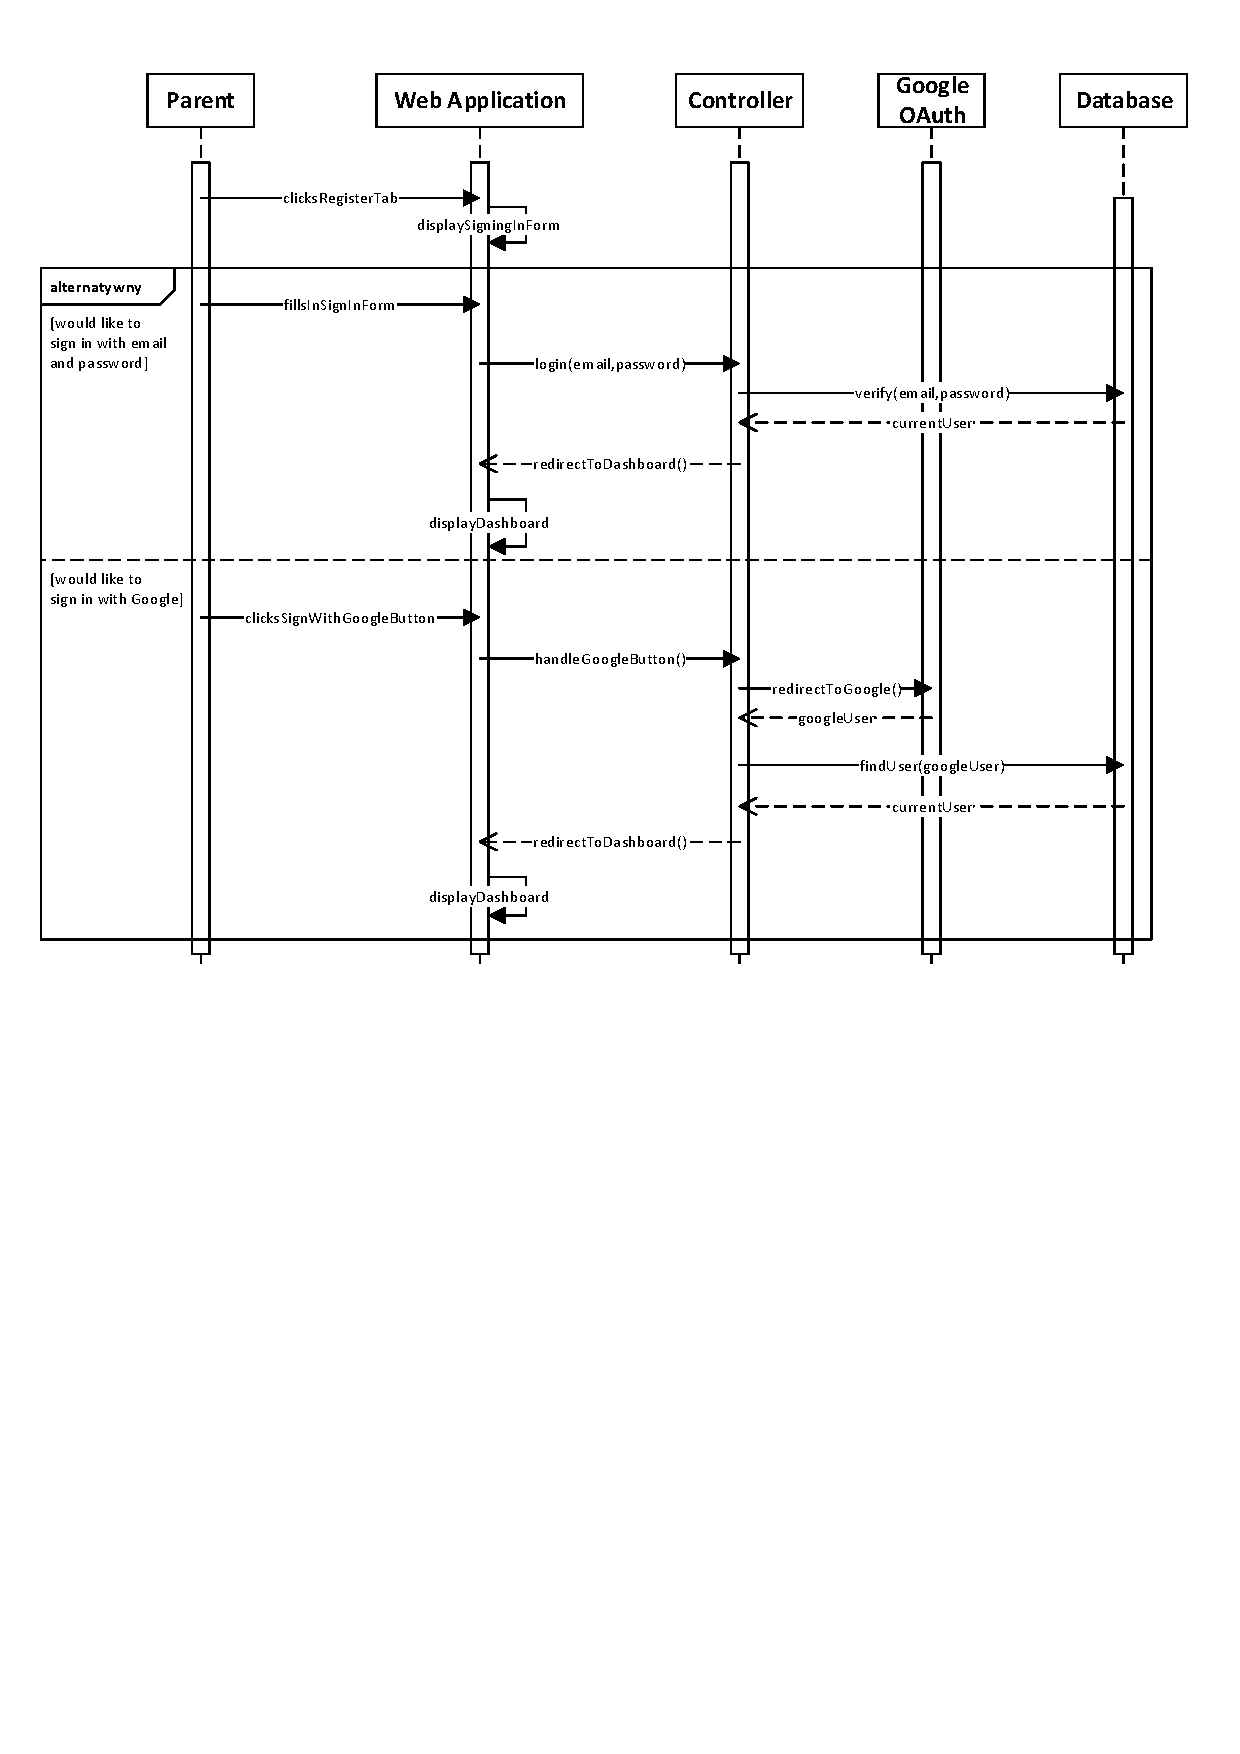
\includegraphics[width=.95\textwidth]{loginSequenceDiagram}
				\end{tabular} 
				\caption{Login Sequence Diagram}
			\end{figure}
		
			\begin{figure}[H] 
				\centering
				\begin{tabular}{c}
					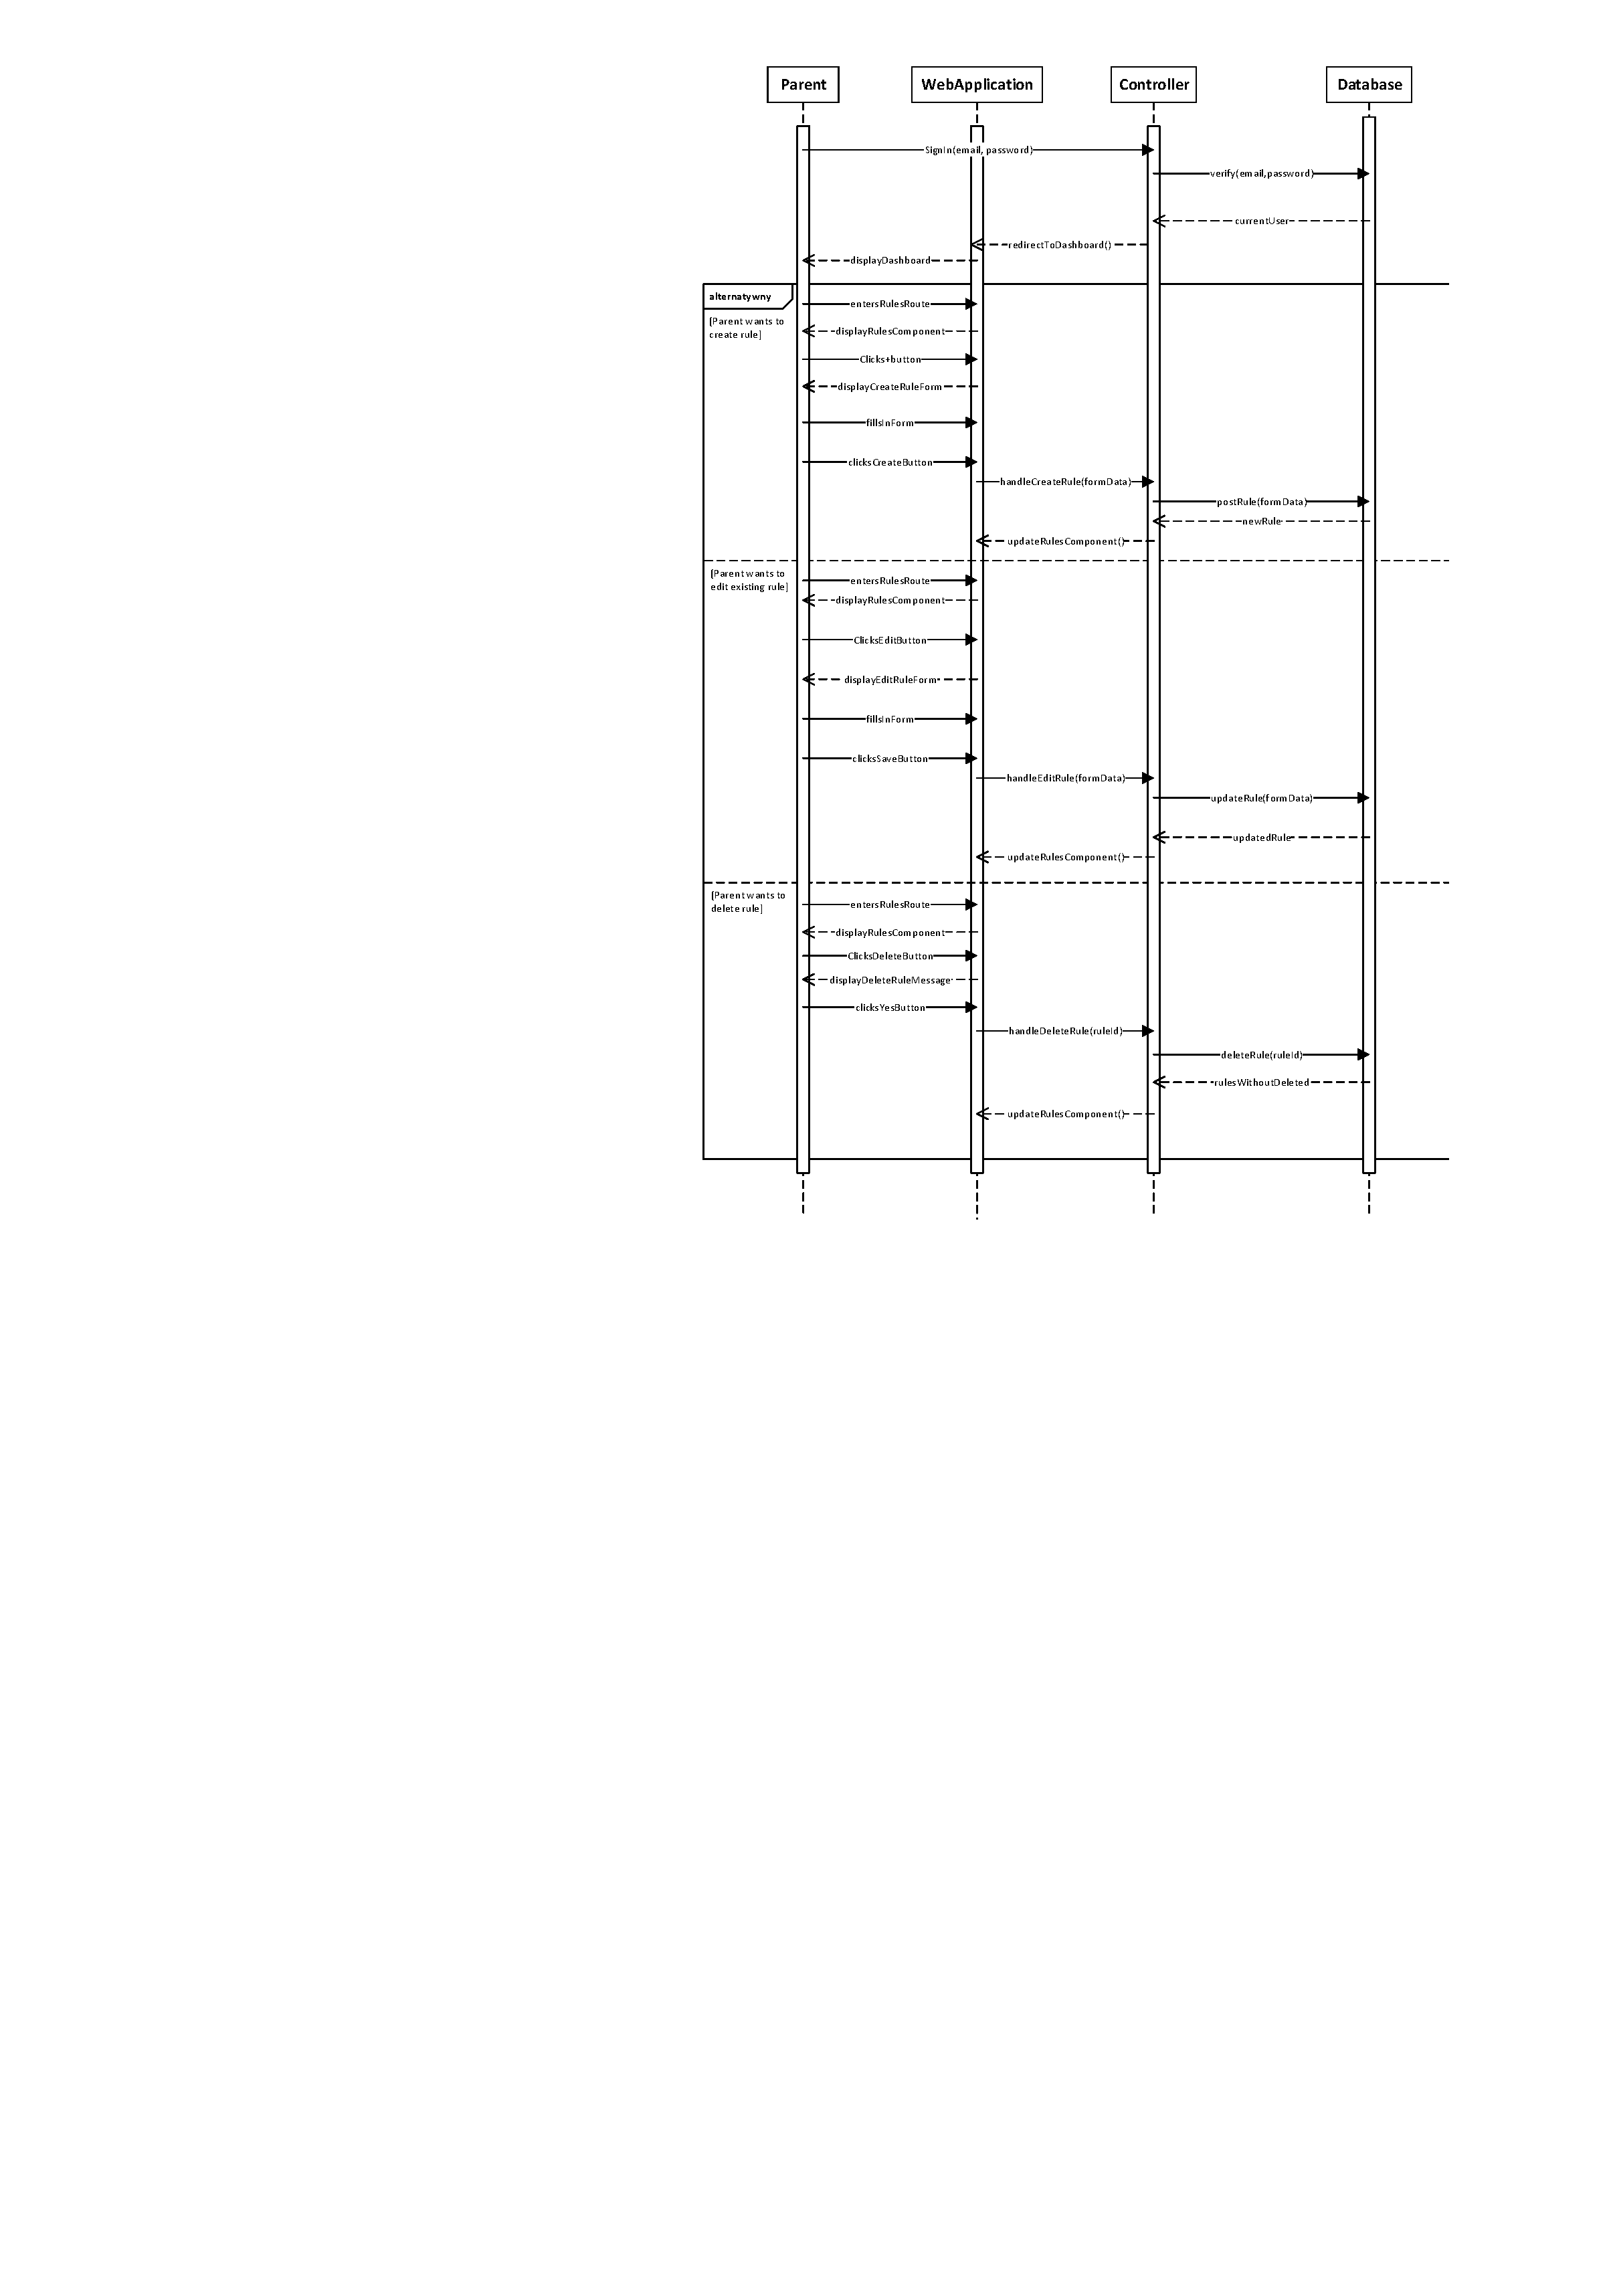
\includegraphics[width=.85\textwidth]{CRUDSequenceDiagram}
				\end{tabular} 
				\caption{CRUD Rules Sequence Diagram}
			\end{figure}
		
			\begin{figure}[H] 
				\centering
				\begin{tabular}{c}
					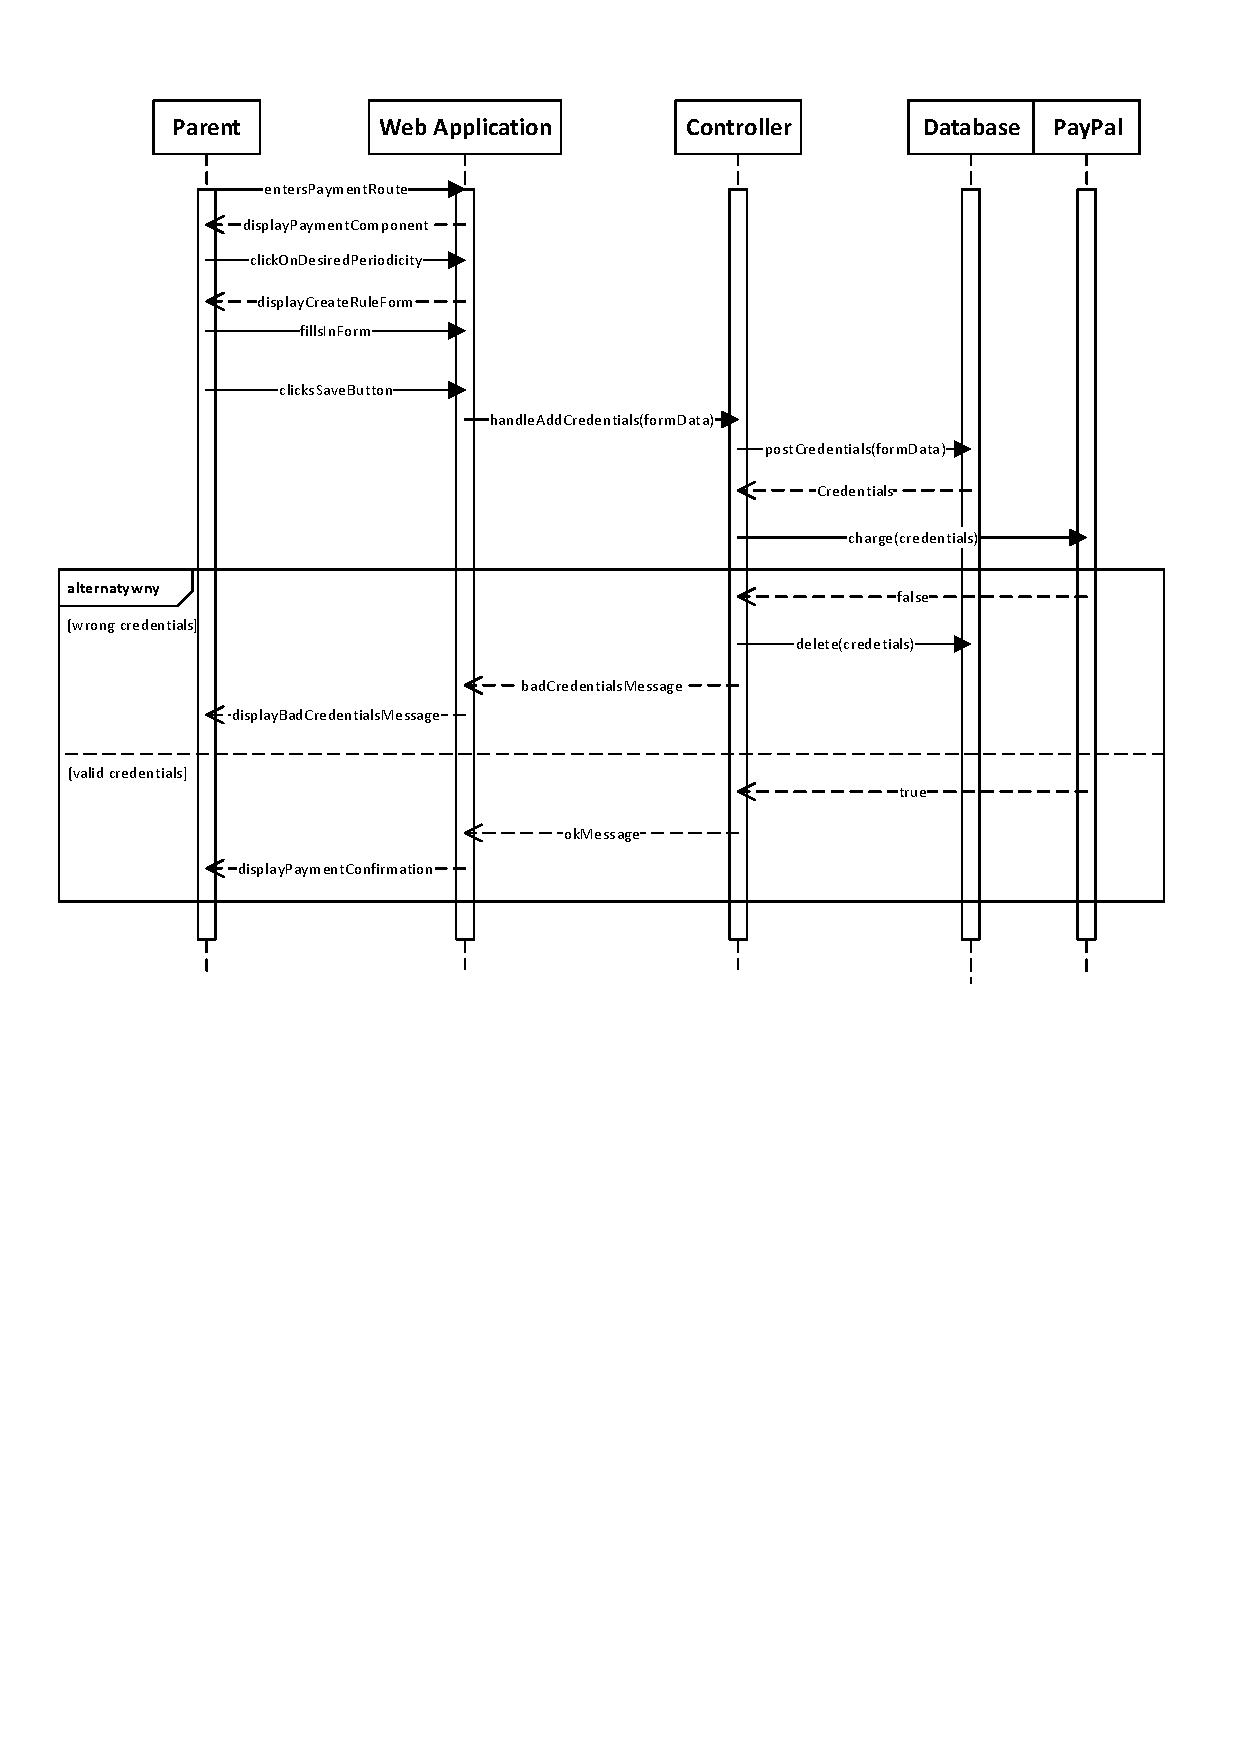
\includegraphics[width=.85\textwidth]{paymentSequenceDiagram}
				\end{tabular} 
				\caption{Payment Rules Sequence Diagram}
			\end{figure}

			\begin{figure}[H] 
				\centering
				\begin{tabular}{c}
					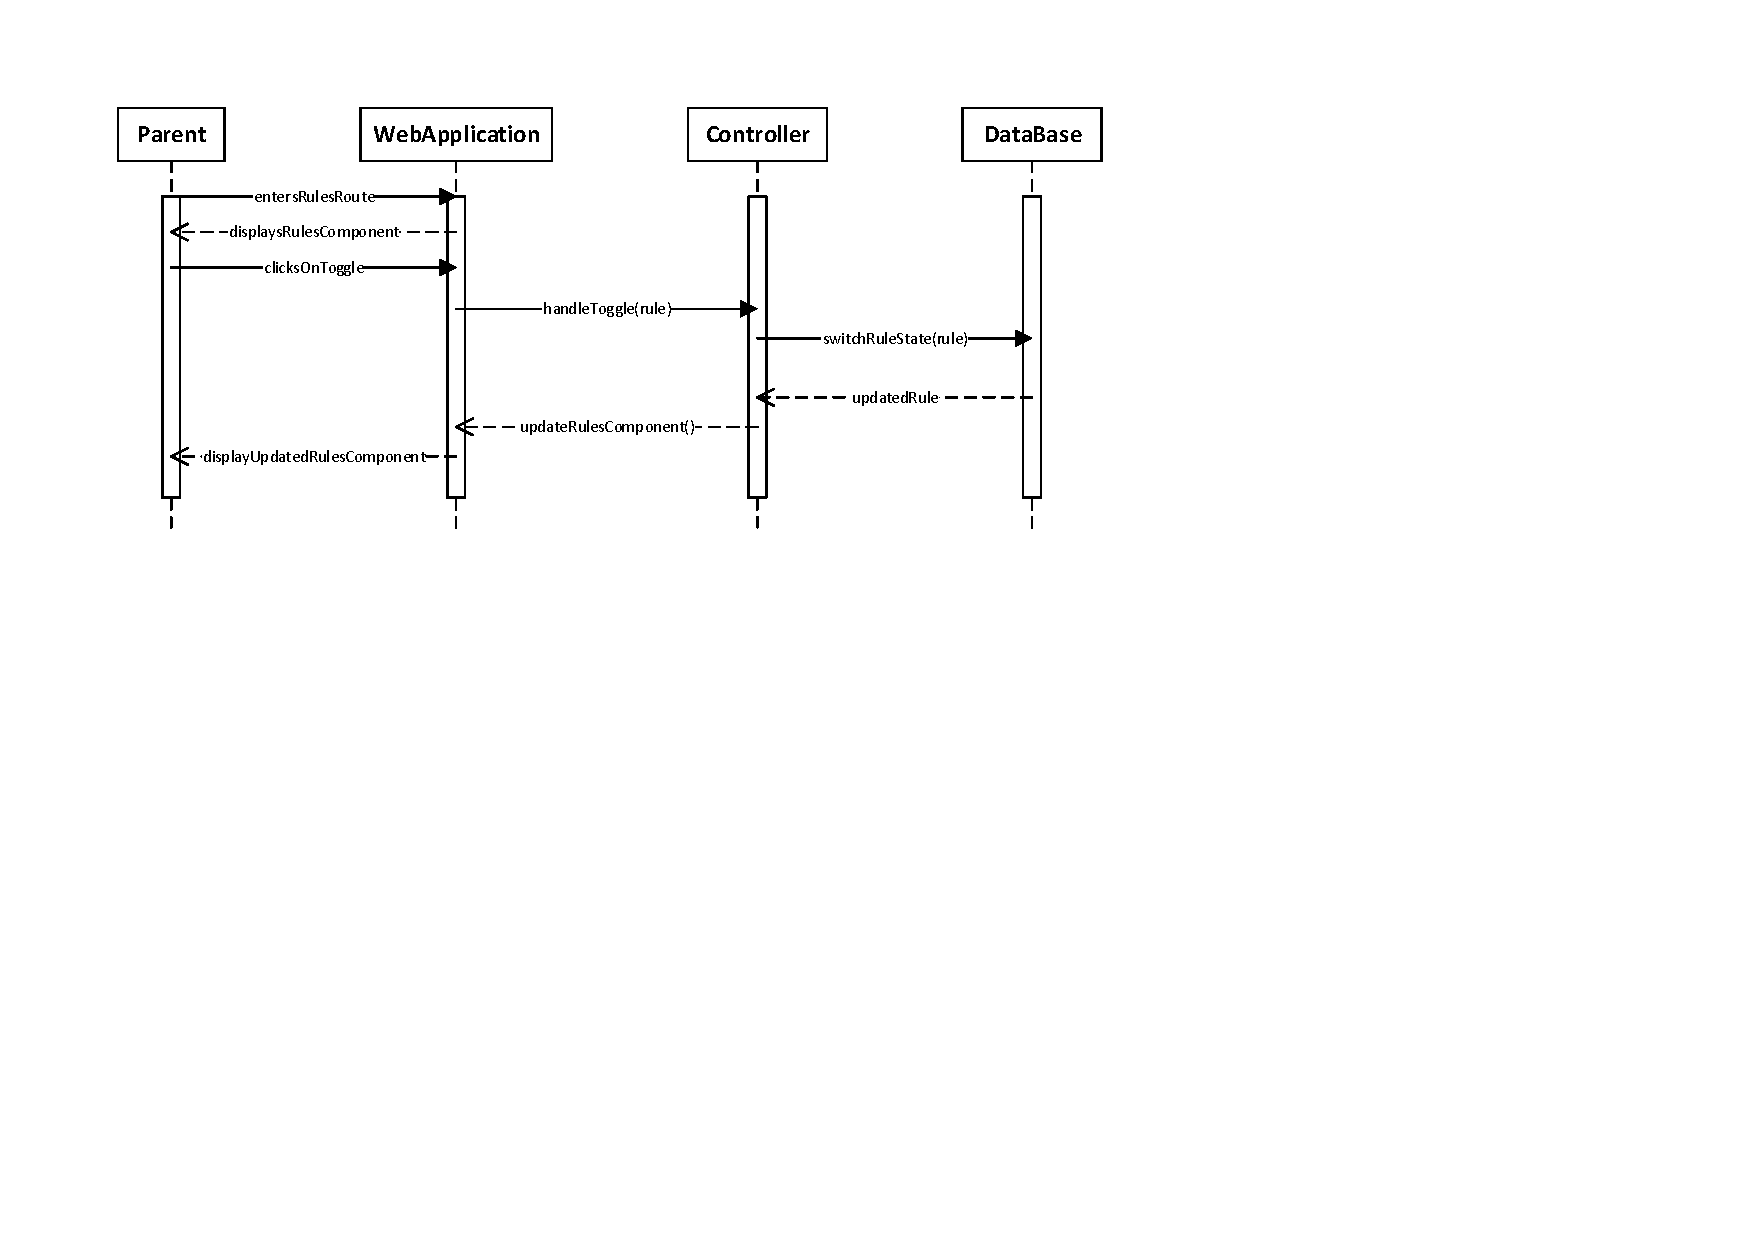
\includegraphics[width=.85\textwidth]{toggleSequence}
				\end{tabular} 
				\caption{Toogle Rule's State Sequence Diagram}
			\end{figure}
		
		\subsection{Server side: API}

			Platform: JavaScript -> NodeJS -> Express

			Our application's modules communicate with server through RESTful API. Our application will send requests to server when user fills forms, and clicks buttons. Server will fetch proper data using axios from MongoDB database on mLab server. Based on fetched data web components will update or user will be redirected to proper route.
			
			\begin{itemize}
				\item \textbackslash api\textbackslash current\_user - current signed in user,
				\item \textbackslash api\textbackslash logout - logging out user,
				\item \textbackslash api\textbackslash googleAuth - signing user in with Google OAuth,
				\item \textbackslash api\textbackslash register - registering new user,
				\item \textbackslash api\textbackslash login - signing user in,
				\item \textbackslash api\textbackslash rules - rules for current user,
				\item \textbackslash api\textbackslash rules\textbackslash create - creating new rule for current user,
				\item \textbackslash api\textbackslash rules\textbackslash read - rule data,
				\item \textbackslash api\textbackslash rules\textbackslash update - updating rule,
				\item \textbackslash api\textbackslash rules\textbackslash delete - deleting rule,
				\item \textbackslash api\textbackslash areas - areas for current user,
				\item \textbackslash api\textbackslash areas\textbackslash create - creating new area,
				\item \textbackslash api\textbackslash areas\textbackslash read - area data,
				\item \textbackslash api\textbackslash areas\textbackslash update - updating area,
				\item \textbackslash api\textbackslash areas\textbackslash delete - deleting area,	
				\item \textbackslash api\textbackslash children - children for current user,
				\item \textbackslash api\textbackslash children\textbackslash create - creating new child,
				\item \textbackslash api\textbackslash children\textbackslash read - child data,
				\item \textbackslash api\textbackslash children\textbackslash update - updating child data,
				\item \textbackslash api\textbackslash children\textbackslash delete - deleting child data.
			\end{itemize}
		
	\section{Data Base}

	\subsection{Diagrams}

		\begin{figure}[H] 
			\centering
			\begin{tabular}{c}
				\includegraphics[width=.95\textwidth]{userDatabase}
			\end{tabular} 
			\caption{Users document schema}
		\end{figure}

		\begin{figure}[H] 
			\centering
			\begin{tabular}{c}
				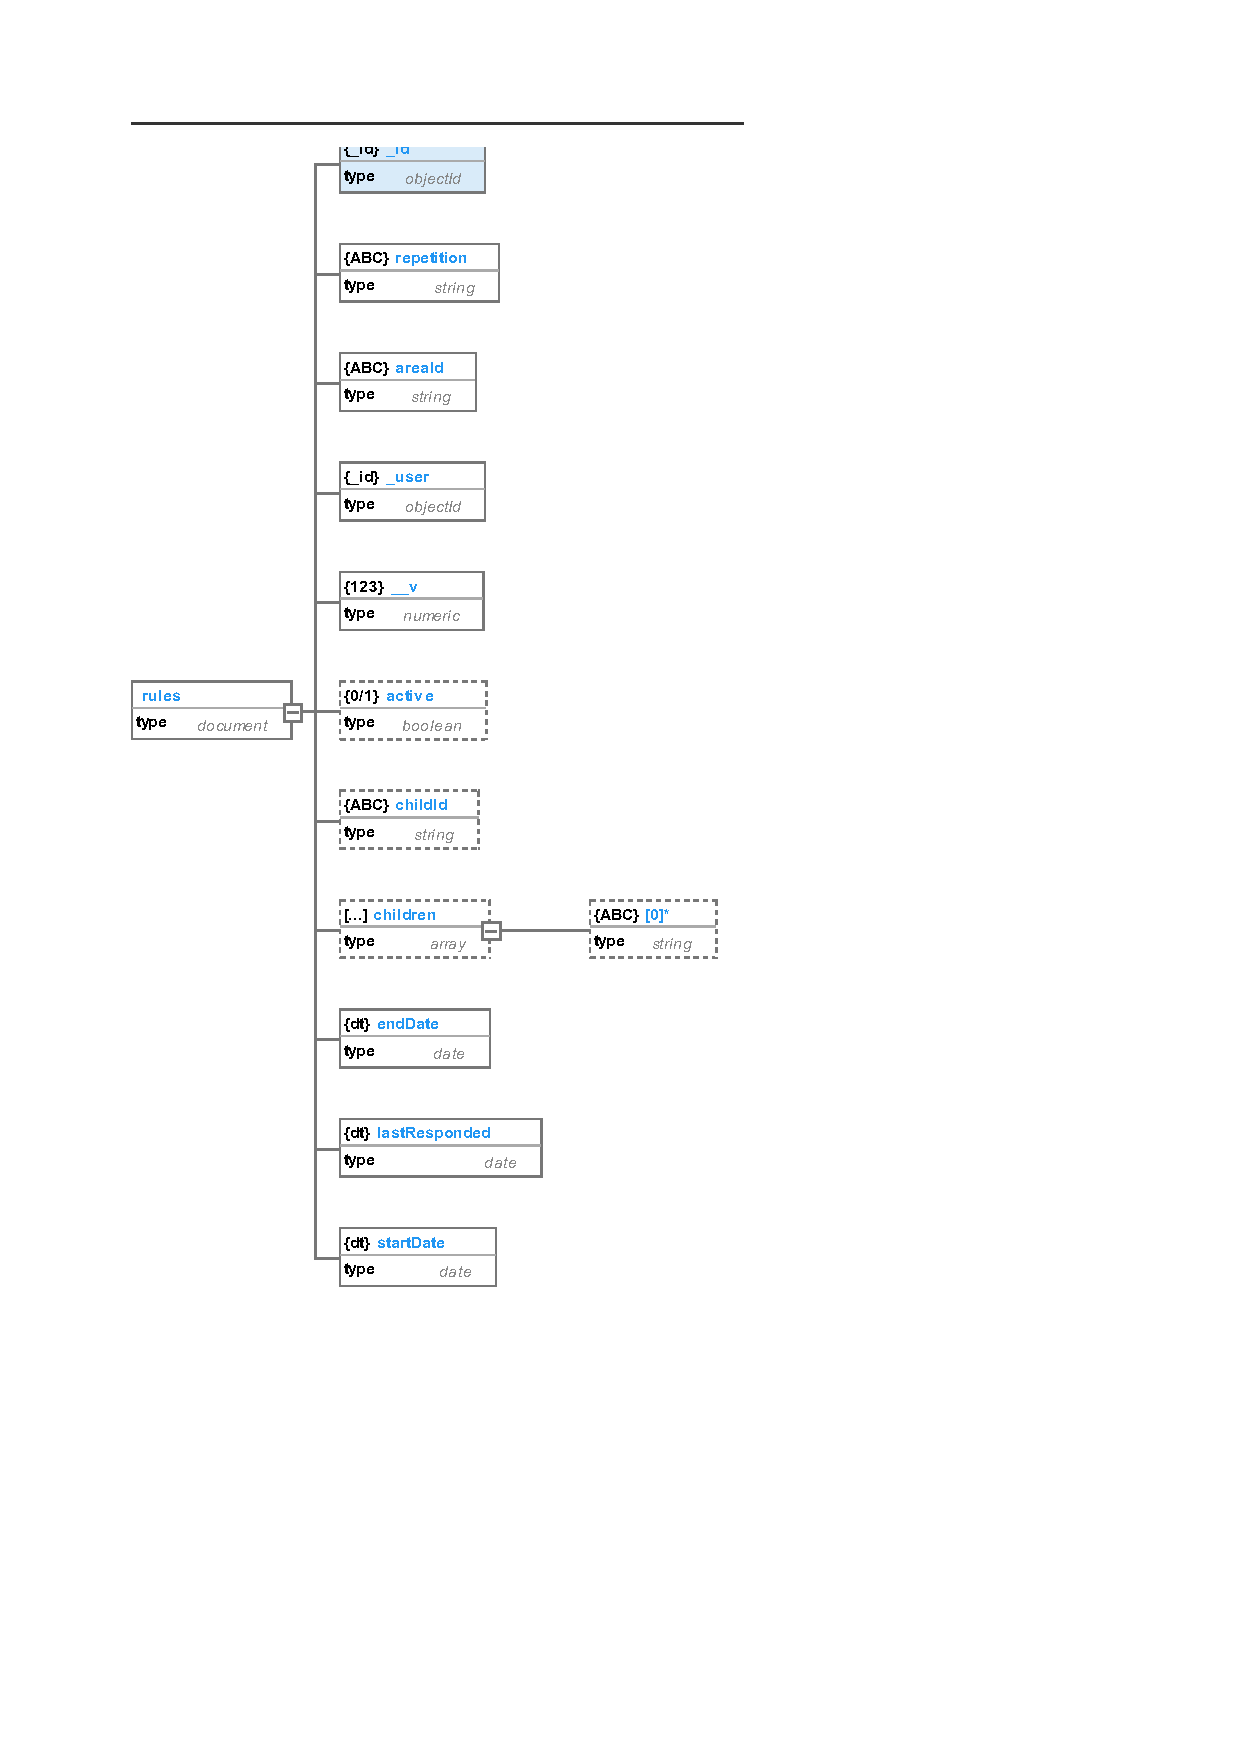
\includegraphics[width=.70\textwidth]{rulesDatabase} 
			\end{tabular} 
			\caption{Rules document schema}
		\end{figure}

	\subsection{Queries for Rules}

		We will show implementation of queries only for rules, because queries of children and areas are implemented in a very analogous way. Rules queries are executed by mongoose library, therefore they are very simple.

		\subsubsection{Create}
			\begin{lstlisting}
				newRule = new Rule({
					startDate,
					endDate,
					repetition,
					areaId,
					lastResponded,
					childId,
					_user
				});
				await newRule.save();
			\end{lstlisting}

		\subsubsection{Read current}
			\begin{lstlisting}
				Rule.find({
					_user,
					startDate: {$lte: Date.now()},
					endDate: {$gte: Date.now()}
				});
			\end{lstlisting}

		\subsubsection{Read all}
			\begin{lstlisting}
				Rule.find({
					_user
				});
			\end{lstlisting}
		
		\subsubsection{Update}
			\begin{lstlisting}
				Rule.updateOne({_id: ruleId},{
					startDate,
					endDate,
					repetition,
					areaId,
					lastResponded: Date.now(),
					childId,
				});
			\end{lstlisting}
		
		\subsubsection{Delete}
			\begin{lstlisting}
				Rule.deleteOne({
					_id
				});
			\end{lstlisting}

\end{document}